% !TEX program = xelatex
\documentclass[UTF8]{ctexrep}
\usepackage{xeCJK}
\setCJKmainfont[BoldFont=HiraginoSansGB-W3, ItalicFont=AdobeKaitiStd-Regular]{FZXSSJW--GB1-0}
\setCJKsansfont{HiraginoSansGB-W6}
\setCJKmonofont{FZLTXHK--GBK1-0}
\CTEXsetup[format+={\raggedright}]{section}

\usepackage{fontspec}
\setmainfont{TimesNewRomanPSMT}
\setsansfont{Verdana}
\setmonofont{Menlo-Regular}

\newfontfamily{\FAB}{Font Awesome 5 Brands Regular}
\setCJKfamilyfont{FZFS}{FZFENSTXJW--GB1-0}
\newfontfamily{\FAFR}{Font Awesome 5 Free Regular}
\def\faGithub{{\FAB \symbol{"F09B}}} % Github
\def\faEmail{{\FAFR \symbol{"F0E0}}} % E-Mail

\usepackage{float}

\usepackage{geometry}
\geometry{a4paper,left=3cm,right=3cm,top=2.5cm,bottom=2.5cm}

\usepackage{fancyhdr}
\pagestyle{fancy}
\fancyhf{}
\chead{\itshape 现代密码学简介}
\rhead{\thepage}
\renewcommand\headrulewidth{0.6pt}

\makeatletter
\renewcommand\chapter{\if@openright\cleardoublepage\else\clearpage\fi
    \thispagestyle{fancy}% original style: plain
    \global\@topnum\z@
    \@afterindentfalse
    \secdef\@chapter\@schapter%
}
\makeatother

\renewcommand{\labelitemii}{$\circ$}

\usepackage{amsmath}
\usepackage{esvect}
\usepackage{bm}
\usepackage{upgreek}
\def \paral {/\!/}
\usepackage{mathtools}
\usepackage{amssymb}
\usepackage{extarrows}
\usepackage{mathrsfs}
\usepackage[amssymb]{SIunits}
\renewcommand{\epsilon}{\varepsilon}
\newcommand{\ext}{\displaystyle}
\newcommand{\arsinh}{\mathrm{arsinh}\,}
\newcommand{\arcosh}{\mathrm{arcosh}\,}
\newcommand{\artanh}{\mathrm{artanh}\,}
\newcommand{\dif}{\mathop{}\!{}\mathrm{d}}
\newcommand{\ic}{\mathrm{i}}
\newcommand{\Tr}{\mathrm{T}}
\newcommand{\ke}{\mathrm{k}}
\newcommand{\p}{\mathrm{p}}
\newcommand{\Z}{\mathbb{Z}}

\def\mathbm#1{{\bm #1}}
\def\vec#1{\vv{\bm #1}}
\def\xvec#1#2{\vv{{\bm #1}_{#2}}}
\def\yvec#1#2{\vv{{\bm #1}^{#2}}}
\def\abs#1{\left| #1 \right|}
\def\pth#1{\left( {#1}\right)}
\def\brack#1{\left[ {#1}\right]}
\def\brace#1{\left\{ {#1} \right\}}
\def\E#1#2{{\mathrm{E}_{#1}\left({#2}\right)}}
\def\D#1#2{{\mathrm{D}_{#1}\left({#2}\right)}}
\def\GF{\mathrm{GF}}
\def\ID{\mathrm{ID}}
\renewcommand{\rem}{{\bfseries Remark}}

\usepackage{amsthm}

\newtheorem{Definition}{\hspace{2em}定义}[chapter]
\newtheorem{theorem}{\hspace{2em}定理}[chapter]

\usepackage[framemethod=tikz]{mdframed}
\newenvironment{prove}{\begin{mdframed}[backgroundcolor=gray!10,roundcorner=8pt]}{\end{mdframed}}

\title{现代密码学简介}
\author{张曙}
\date{\today}

\usepackage[absolute]{textpos}

\usepackage[unicode]{hyperref}
\hypersetup{pdfauthor={张曙},
pdftitle={现代密码学简介},
hidelinks
}
\begin{document}
\begin{titlepage}
\vspace*{9em}{\centering\Huge\CJKfamily{FZFS} 现代密码学简介\par}
\vspace{5em}{\centering\Large \textbf{张曙}\par}
\vspace{3em}{\centering\faGithub\quad\texttt{\href{https://github.com/Evian-Zhang}{https://github.com/Evian-Zhang}}\par\centering\faEmail\quad\texttt{\href{mailto:evianzhang1999@gmail.com}{evianzhang1999@gmail.com}}\par}
\begin{textblock}{10}[0,0](3,14)
在GitHub上查看本项目:\faGithub\quad\texttt{\href{https://github.com/Evian-Zhang/Introduction-to-modern-cryptography}{Evian-Zhang/Introduction-to-modern-cryptography}}
\end{textblock}
\end{titlepage}
\tableofcontents
\thispagestyle{fancy}
% !TEX root = ../../现代密码学简介.tex
\chapter{绪论}
\section{什么是密码学}
如果我们要求一个从未接触过密码学的人处理一段文字,把这段文字尽可能地加密,让别人无法破解。那么,大多数人在深思熟虑之后,总能提出一些加密算法。这时候,一般人的思路可能会有几个方向。\par
有的人的方向是把这段文字中的字母之间通过各种复杂的运算进行组合。比如说,把要加密的文字中每两个字母在字母表中的位置进行相加,形成密码。比如说,``cryptography''中,``cr''变成了$3+18=21$, ``yp''变成了$25+16=41$, ``cryptography''对应的密码就是``214135252133''。但这样的密码,显然忽略了一点:密码的可解密性。我们之所以要进行加密,是为了安全地传递信息。但接收信息者必须要有解密的方法。但这种加密方式则没有对应的解密方法。所以说,这不是一个合格的加密方式。\par
这时,足够聪明的人,则考虑到了解密的方法。他们想出了一些类似于古代使用的加密方法。比如说,著名的凯撒密码:把一段由英文字母组成的语句,每个字母都在字母表中往后移3个位置。``veni vidi vici''也就变成了``yhql ylgl ylfl''. 这种密码的解密方法,也就是每个字母在字母表中向前移动3个位置。当问起这种密码体制里最重要的是什么,大部分人都会说是加密算法。如果把加密算法告诉了别人,那这种密码就相当于被破解了。\par
如果进而问起一个密码体制的组成,大部分人的回答,就是加密算法。也许有些自诩比普通人聪明一点的人,还会加上一个解密算法,也就是,将处理过后的密码变为正常文字的算法。如果用$m$代表要被加密的文字,$c$代表被加密出来的密码,$\mathrm{E}()$代表加密算法,$\mathrm{D}()$代表解密算法,那么大多数人理解的密码学,本质就是以下这两个式子:
\begin{gather*}
    c=\mathrm{E}\pth{m}\\
    m=\mathrm{D}\pth{c}
\end{gather*}

\subsection{密钥}
但是,我们考虑一下实际的情况。根据我们之前的常识,会发现,如果要用密码来传递信息,首先通信的双方必须要在一个安全信道中传递一些额外的信息。比如说,告诉接收者加密的方式,或者更直接地,告诉接收者解密算法。不存在一种加密的方式,能不事先通过安全信道传递信息,而使得只有接收者能够解密。那么,为了使通信更加安全,通信双方对安全信道的使用应该尽可能少。如果Alice和Bob使用凯撒密码进行通信,而Alice事先在安全信道中要对Bob说“我的这种加密方式是把一段由英文字母组成的语句,每个字母都在字母表中往后移3个位置。”这段话是如此之长,而如果考虑是在战场上,由通信员用摩尔斯电码发送,那么花费的这么长的时间显然是不合理的。再者,现代的通信方式一般都是把信息编码成二进制进行传递,那么,相比把一段话编码成二进制,不如找一些数字来代表这个密码。在我们的这段思想博弈中,一个重要的概念呼之欲出。\par
拿凯撒密码为例,在其加密算法中,还有一个关键的量:3. 试想,如果通信双方Alice和Bob, Alice在场的所有人她用的是凯撒密码的加密方式加密她的话,又在安全信道中告诉Bob``4'', 意味着她使用的凯撒密码里,是将每个字母在字母表的位置上向后移动4个位置。那么,即使在场有人能偷听到Alice给Bob的密码,也无法破解Alice想说的是什么,只有掌握了规则“向后移动4个位置”的Bob, 才能正确地破解密码。\par
如果还是按照之前的说法,一个密码体制包括加密算法和解密算法,那么向后移动3个位置的凯撒密码和向后移动4个位置的凯撒密码,就成了两个密码体制。但是,这两种加密方式是极其类似的,差别也就只在于一个向后移动3个位置,一个向后移动4个位置。我们对于这些密码的研究,也许也就十分类似。因此,把这两种加密方式归类为同一种密码体制,似乎是更好的选择。因此,\textbf{密钥}就应运而生了。所谓密钥,我们可以粗略地理解成加密算法、解密算法中的参数,也就是我们之前说的3、4. 通过一个密码体制通信的双方,需要首先在保密信道中确定密钥。而一个密码体制,也就可以由加密算法、解密算法和密钥构成。因此,如果以$k$代表密钥,那么之前的式子就变成了
\begin{gather*}
    c=\E{k}{m}\\
    m=\D{k}{c}
\end{gather*}

这也就是现在通用的密码学。\par
那么我们思考几个问题:在一次加密通信过程中,加密算法和解密算法中使用的密钥是否必须要相同?密钥是否只能是一个数?可不可以没有密钥?\par
针对第一个问题,确实存在某些高端的技巧,使得加密算法和解密算法使用的密钥是不同的。事实上,在密码学领域中,根据加密算法和解密算法使用的密钥是否相同,人们将加密方式分为对称加密与非对称加密,分别对应使用同一密钥和使用不同密钥。非对称加密方式也许难以理解,我们也会在充分学习对称加密后再介绍非对称加密。所以,我们接下来讨论的对称加密过程中,请大家记住,加密算法和解密算法使用的是相同的密钥。\par
此外,对于对称加密算法,密钥也并不一定是一个数。比如说,加密算法
\[\E{a, b}{m}=am+b\]
其密钥为$\pth{a, b}$, 但我们仍认为其使用单一密钥,也就是说,把$\pth{a, b}$看作一个密钥。\par
此外,可不可能不存在密钥呢?确实有这样的密码体制,但这样却也十分不安全。比如说,加密算法
\[\mathrm{E}\pth{m}=m\]
就是一个无密钥的加密算法。
\section{密码体制的基本要素}
根据之前的讨论,我们就可以得出一个密码体制的基本要素:
\begin{itemize}
    \item 明文空间$\mathcal{M}$\par
    所有可以被加密算法加密的元素组成的集合,加密算法的定义域。明文空间的元素叫做明文$m\in\mathcal{M}$.\par
    例如,在凯撒密码中,明文空间就为所有由英文字母组成的字符串。
    \item 密文空间$\mathcal{C}$\par
    所有可以由加密算法输出的元素组成的集合,加密算法的值域。密文空间的元素叫做密文$c\in\mathcal{C}$.\par
    我们需要注意到的是,这里的值域,可以理解成二元函数$\mathrm{E}\pth{k, m}$的值域。比如说,对于加密算法
    \[\E{k}{m}=m^2+k^2\]
    其密文空间为$[0, +\infty)$而非$[k^2, +\infty)$.
    \item 密钥空间$\mathcal{K}$\par
    所有密钥组成的集合。密钥空间的元素叫做密钥$k\in\mathcal{K}$.\par
    在非对称加密中,密钥空间分为加密密钥空间和解密密钥空间。
    \item 加密算法$\E{k}{m}$\par
    根据密钥生成的特定算法,将明文转化为密文。
    \item 解密算法$\D{k}{c}$\par
    根据密钥生成的特定算法,将密文转化为明文。\par
    对于对称加密算法,也就是只使用一个密钥的加密体制,解密算法与加密算法满足
    \[\D{k}{\E{k}{m}}=m\]
\end{itemize}

在我们讨论密码体制的一些性质时,密钥生成算法有时也是必要的。什么是密钥生成算法呢?回忆之前Alice和Bob的例子,凭什么Alice选择的密钥是4而不是25呢?这就涉及到了密钥生成算法。在这个例子中,密钥生成算法就是Alice自己想到哪个密钥就输出哪个密钥。但是,从严格意义上来讲,密钥生成算法是一种概率算法。所谓概率算法,就是在算法的步骤中涉及到了某些概率。比如说,在某个密钥生成算法中,在$(0, 1)$中等概率随机生成一个数$t$, 而生成的密钥$k$满足
\[
    k=\begin{cases}1&t\in\pth{0.5, 1}\\0&t=0.5\\-1&t\in\pth{0, 0.5}\end{cases}
\]

这就是一个典型的概率算法。其特点就是在两次运行中输出的结果不一定相同。\par
因此,我们称一个加密方案包含三个要素:加密算法$\mathrm{E}$, 解密算法$\mathrm{D}$, 密钥生成算法$\mathrm{G}$. 根据定义,我们可以说,一个密码体制由一个加密方案$\pth{\mathrm{E}, \mathrm{D}, \mathrm{G}}$及一个明文空间$\mathcal{M}$完全定义。\par
因此,Alice和Bob的一次加密通信的过程包括:
\begin{enumerate}
    \item Alice根据密钥生成算法$\mathrm{G}$生成密钥$k\in\mathcal{K}$.
    \item Alice通过安全信道将$k$告诉Bob.
    \item Alice将想要传达的明文$m\in\mathcal{M}$根据加密算法加密成密文$c=\E{k}{m}$告诉Bob.
    \item Bob根据之前Alice告诉自己的$k$、密文$c$及解密算法得出明文$m=\D{k}{c}$
\end{enumerate}

那么,在一个密码体制中,哪个最重要呢?是不是之前我们说的加密算法呢?这里,就不得不提Kerckhoffs原则。用现代的语言来说,Kerckhoffs原则阐述的是:
\begin{quote}
    提倡安全性不能建立在对算法的保密上。
\end{quote}

也就是说,我们如果要证明一个加密体制的安全性,不能指望算法的保密性。我们应默认加解密算法可以被所有人知道(事实上也确实如此)。也就是说,真正值得保密的,是密钥。如果潜在的敌手获得密钥,那么根据公开的解密算法,那么他就可以从窃得的密文中获得明文。
\subsection{弱密钥与半弱密钥}
在我们构造密码体系的时候,有的人会想,利用已有的密码体系加密两次怎么样?即:
\[\E{k}{\E{k}{m}}\]
或者
\[\E{k_1}{\E{k_2}{m}}\]
的安全性如何?\par
这里提出了弱密钥与半弱密钥的概念:
\begin{Definition}
对于加密方式$\E{k}{m}$, 若密钥$k$使得对于任意$m\in\mathcal{M}$, 有
\[\E{k}{\E{k}{m}}=m\]
则称$k$为弱密钥。\par
若密钥$k_1, k_2$若密钥$k$使得对于任意$m\in\mathcal{M}$, 有
\[\E{k_1}{\E{k_2}{m}}=m\]
则称$k_1, k_2$为一对半弱密钥。
\end{Definition}

由上述定义可知,如果我们想要利用已有的密码体系加密两次,那么一定要避开的就是弱密钥与半弱密钥。
\section{经典密码}
\subsection{基础概念}
我们讨论了密码体制的基本要素之后,就可以介绍一些经典的密码,让大家更好地理解这些术语了。\par
值得指出的是,这些密码都是古代欧洲人的研究成果,当时并没有如今“数字化”的概念。因此,这些密码,都是针对拉丁字母进行的加密。因此,我们首先要引入一些概念:\par
函数$C\pth{m}$将拉丁字母$m$映射到它在字母表中的位置上,比如$C(a)=1, C(z)=26$. 函数$I\pth{n}$将位于$1$和$26$之间的数字映射到字母表中相应位置的拉丁字母上,比如$I(1)=a, I(26)=z$.\par
在讨论经典密码时,一些极其基础的数论记号及知识可以让我们更加方便、更加简洁地叙述、理解这些经典密码。\par
我们用$\gcd\pth{a, b}$表示$a$与$b$的最大公因数。\par
用$a\bmod{b}$表示整数$a$除以$b$后的余数(取值范围为$0$到$b-1$), 比如说$15\bmod{6}=3, 12\bmod{6}=0, \pth{-4}\bmod{6}=2$.\par
若$a\bmod{b}=0$, 即$a$能整除$b$, 我们则记为$a\mid b$. 如$2\mid 4, 3\nmid 4$.\par
若$\pth{a-b}\mid c$, 我们则称$a$与$b$模$c$同余,记作$a\equiv b\pmod{c}$. 如$16\equiv 23\pmod{7}$.\par
对于整数$a, b$, 若存在整数$c$使得$ac\equiv 1\pmod{b}$, 则称$c$为$a$在模$b$时的逆,记作$a^{-1}$. 并非所有的整数都有逆,如在模$4$的情况下,整数$2$就没有逆。对于整数$a, b$, 在模$b$时$a$存在逆的充分必要条件为$\gcd\pth{a, b}=1$.
\subsection{单表代换密码}
单表代换密码的典型,就是凯撒密码。如果用我们上述的记号来表示凯撒密码的过程,那么如果设明文为字符串``$m_1m_2\cdots m_n$'',密文为字符串``$c_1c_2\cdots c_n$'', $m_i, c_i$均代表一个拉丁字母。凯撒密码的加密算法
\begin{equation}
    c_i=\E{}{m_i}=C\pth{\pth{I\pth{m_i}+3}\bmod{26}}
\end{equation}

解密算法
\begin{equation}
    m_i=\D{}{c_i}=C\pth{\pth{I\pth{c_i}-3}\bmod{26}}
\end{equation}

它通过对字母表中每个字母进行固定的代换,得到密码。单表替换密码则是凯撒密码的推广,引入了密钥。从数学意义上,可以作如下定义:\par
设明文为字符串``$m_1m_2\cdots m_n$'',密文为字符串``$c_1c_2\cdots c_n$'', $m_i, c_i$均代表一个拉丁字母。如果把整数对$\pth{a, b}$作为密钥,其中$a\neq 0$, 那么其加密算法
\[c_i=\E{a, b}{m_i}=C\pth{\pth{aI\pth{m_i}+b}\bmod{26}}\]

解密算法
\[m_i=\D{a, b}{c_i}=C\pth{\pth{a^{-1}\pth{I\pth{c_i}-b}}\bmod{26}}\]
其中$a^{-1}$为$a$模$26$的逆。\par
事实上,如果我们令$n_i=I\pth{m_i}, q_i=I\pth{\E{a, b}{m_i}}, e_i=I\pth{\E{a, b}{m_i}}, d_i=I\pth{\D{a, b}{\E{a, b}{m_i}}}$, 那么
\[q_i\equiv an_i+b\pmod{26}\]

故
\begin{align*}
    d_i&\equiv a^{-1}\pth{q_i-b}\\
    &\equiv a^{-1}\pth{an_i+b-b}\\
    &\equiv n_i\pmod{26}
\end{align*}

也就是说,
\[I\pth{\D{a, b}{\E{a, b}{m_i}}}\equiv m_i\pmod{26}\]

故
\[\D{a, b}{\E{a, b}{m_i}}=m_i\]

这也就证明了这个加密算法是正确的算法。\par
让我们不要再纠结于繁琐的数学符号,我们来从直观上看一看这个加密算法。任意取一个密钥,比如说,$a=3, b=7$, 就会对应的生成一张加密表和解密表:
\begin{table}[H]
    \centering
    \caption{$a=3, b=7$时的加密表}
    \begin{tabular}{c|c|c|c|c|c|c|c|c|c|c|c|c|c}\hline
        明文&a&b&c&d&e&f&g&h&i&j&k&l&m\\
        密文&h&k&n&q&t&w&z&c&f&i&l&o&r\\\hline
        明文&n&o&p&q&r&s&t&u&v&w&x&y&z\\
        密文&u&x&a&d&g&j&m&p&s&v&y&b&e\\\hline
    \end{tabular}
\end{table}
\begin{table}[H]
    \centering
    \caption{$a=3, b=7$时的解密表}
    \begin{tabular}{c|c|c|c|c|c|c|c|c|c|c|c|c|c}\hline
        密文&a&b&c&d&e&f&g&h&i&j&k&l&m\\
        明文&p&y&h&q&z&i&r&a&j&s&b&k&t\\\hline
        密文&n&o&p&q&r&s&t&u&v&w&x&y&z\\
        明文&c&l&u&d&m&v&e&n&w&f&o&x&g\\\hline
    \end{tabular}
\end{table}

那么我们根据这张表,就可以很快地进行加密和解密的工作了。\par
我们再回到之前所说的加密体制的基本要素:其明文空间$\mathcal{M}$为由拉丁字母组成的任意长度的字符串组成的集合,密文空间$\mathcal{C}=\mathcal{M}$. 密钥空间$\mathcal{K}=\brace{\pth{a, b}\mid a, b\in \Z, \gcd\pth{a ,26}=1}$(这里$\gcd\pth{a, 26}=1$的条件是因为解密算法中要求$a$模$26$的逆存在。).
\subsection{单表代换密码的破解}
上述的单表代换密码看似十分安全,但是如果用来加密由拉丁字母组成的用语言逻辑形成的一句话时,却有一个致命的弱点。虽然这些密码不会直接暴露明文,但却会暴露明文中各个字母出现的频率。我们知道,在任何一门由字母组成的语言文字中,每个字母出现的频率在语句十分长时是趋向于一个定值的。比如说,在英文中,有一个著名的短语:``ETAOIN SHRDLU''. 这个短语是英文中出现频率最高的12个字母,从高到低排列。根据这些频率,就可以找到破解这种密码的方法。\par
为什么暴露明文出现的频率就会使加密系统不安全呢?我们可以用一个例子来说明:我们利用单表代换密码的原理,加密东南大学的校徽:
\begin{figure}[H]
\centering
\begin{minipage}[t]{0.49\textwidth}
\centering

\includegraphics[width=10em]{chapters/chapter_1/Caesar_origin.jpg}
\caption{单表代换加密前}
\end{minipage}
\begin{minipage}[t]{0.49\textwidth}
\centering

\includegraphics[width=10em]{chapters/chapter_1/Caesar_result.jpg}
\caption{单表代换加密后}
\end{minipage}
\end{figure}

显而易见,加密效果近似于无。\par
利用这个原理,有两种最常用的方法:频率分析法与巧合指数法。
\subsubsection{频率分析法}
假设利用单表代换密码加密的语言为英文,那么根据统计学家的知识,英文字母出现的频率从高到低依次是``ETAOIN SHRDLU''. 如果我们可以统计出一个相当长的密文中各个字母出现的频率,那么极有可能出现频率最高的字母对应的就是明文中的``E''. 这就是频率分析法的基本思想。
\subsubsection{巧合指数法}
巧合指数法的想法非常直接:对于一段文字,任意取两个字母,这两个字母相同的概率称为巧合指数$\mathrm{IC}$。可以证明,对于一段长度为$N$的文字,共有$c$个字母,每个字母出现的次数为$n_i$, $i=1, 2, \ldots, c$. 那么巧合指数的值为
\begin{equation}
    \mathrm{IC}=\frac{\ext\sum_{i=1}^cn_i\pth{n_i-1}}{N\pth{N-1}}
\end{equation}

如果这段文字充分长,那么我们有
\begin{equation}
    \frac{\ext\sum_{i=1}^cn_i\pth{n_i-1}}{N\pth{N-1}}\approx\frac{\ext\sum_{i=1}^cn_i^2}{N^2}
\end{equation}

如果记$\ext p_i=\frac{n_i}{N}$表示第$i$个字母在这段文字中出现的频率,那么
\begin{equation}
    \mathrm{IC}\approx\sum_{i=1}^cp_i^2
\end{equation}

而我们先前提到,统计学家已经统计出在英文文本中各个字母出现的频率,因此,带入上述式子,可以得出英文文本的巧合指数$\mathrm{IC}\approx 0.0686$. \par
接着我们统计加密过后的密文的巧合指数,假设密钥为$k$, 我们对$k=0, 1, \ldots, 25$依次去试,如果出现了解密后的文本的巧合指数接近于$0.0686$, 就说明这个$k$有很大可能是密钥。
\subsection{多表代换密码}
为了进一步提高安全性,古代的人们想到也许一张表并不足够安全,不妨使用多张表。因此,多表代换密码应运而生。\par
假设一共有$t$张加密表,人们是怎么做的呢?从明文的第一个字符开始,第一个字符使用第一张加密表进行加密,第二个字符使用第二张加密表进行加密,以此类推,第$t$个字符使用第$t$张加密表进行加密。到了第$t+1$个字符,则又回到第一张加密表进行加密。用数学的语言怎么叙述这件事呢?\par
对于明文字符串$M=m_1m_2\cdots m_n$, 我们要求其长度满足$n=tp$. 我们将明文字符串等分成$p$个列向量$M_1, M_2, \ldots, M_p$, 其中$M_i=\pth{m_{p(i-1)+1}, m_{p(i-1)+2}, \ldots, m_{p(i-1)+t}}^{\mathrm{T}}$. 对密文字符串$C$也作同样的划分$C_1, C_2, \ldots, C_p$. 取密钥为$\pth{A, B}$, 其中矩阵$A$为$t\times t$的可逆矩阵,且满足$\gcd\pth{\abs{A}, 26}=1$, $B$为$t$维列向量。\par
那么多表代换密码的加密算法为
\begin{equation}
    C_i=\E{A, B}{M_i}=C\pth{\pth{AI\pth{M_i}+B}\bmod{26}}
\end{equation}

解密算法为
\begin{equation}
    M_i=\D{A, B}{C_i}=C\pth{\pth{A^{-1}I\pth{C_i-B}}\bmod{26}}
\end{equation}

其中$A^{-1}$满足
\[A^{-1}A\bmod{26}=\pth{\begin{array}{cccc}1&0&\cdots &0\\0&1&\cdots&1\\\vdots&\vdots&\ddots &\vdots\\0&0&\cdots&1\end{array}}\]

我们可以用一个具体的例子来理解这些抽象的公式:\par
假设我们一共有三张表,分别使用密钥为$\pth{1, 1}, \pth{3, 3}, \pth{5, 7}$的单表替换密码生成。明文字符串$M=m_1m_2\cdots m_n$的长度$n=3p$. 我们将其等分为$p$个列向量$M_1, M_2, \ldots, M_p$, 其中$M_i=\pth{m_{p(i-1)+1}, m_{p(i-1)+2}, m_{p(i-1)+3}}^{\mathrm{T}}$. 对于密文字符串$C$也作同样的划分$C_1, C_2, \ldots, C_p$. 取
\[A=\pth{\begin{array}{ccc}1&0&0\\0&3&0\\0&0&5\end{array}}, B=\pth{\begin{array}{c}1\\3\\7\end{array}}\]
为密钥。\par
那么其加密算法为
\begin{align*}
    \pth{\begin{array}{c}c_{p(i-1)+1}\\c_{p(i-1)+2}\\c_{p(i-1)+3}\end{array}}=C_i&=\E{A, B}{M_i}=\pth{\begin{array}{ccc}1&0&0\\0&3&0\\0&0&5\end{array}}M_i+\pth{\begin{array}{c}1\\3\\7\end{array}}\bmod{26}\\
    &=\pth{\begin{array}{c}m_{p(i-1)+1}+1\\3m_{p(i-1)+2}+3\\5c_{p(i-1)+3}+7\end{array}}\bmod{26}
\end{align*}

其解密算法为
\[M_i=\D{A, B}{C_i}=\pth{\begin{array}{ccc}1&0&0\\0&9&0\\0&0&21\end{array}}\pth{C_i-\pth{\begin{array}{c}1\\3\\7\end{array}}}\bmod{26}\]

那么我们可以看到,从明文的第一个字符开始,每隔三个字符的第一个字符使用的加密方法为$c_{p(i-1)+1}=\pth{m_{p(i-1)+1}+1}\bmod{26}$, 第二个字符使用的加密方法为$c_{p(i-1)+2}=\pth{3m_{p(i-1)+2}+3}\bmod{26}$, 第三个字符使用的加密方法为$c_{p(i-1)+3}=\pth{5m_{p(i-1)+3}+7}\bmod{26}$. 这也就是我们设计多表代换密码的原意。\par
我们发现,在上述例子中,密钥里的$A$似乎有许多$0$的位置。但是,我们之前在数学上严格定义多表代换密码的时候,并没有要求这些位置一定要是$0$. 事实上,这些位置如果不是$0$,就意味着密文中特定位置的字符并不是由明文中对应位置的字符确定,而是明文中对应位置与前后位置的字符一起确定。这也是可行的。\par
多表代换密码也是不安全的。我们利用多表代换密码同样加密上面提到的东南大学校徽,得到的结果也很不理想:
\begin{figure}[H]
\centering
\begin{minipage}[t]{0.49\textwidth}
\centering

\includegraphics[width=10em]{chapters/chapter_1/Caesar_origin.jpg}
\caption{多表代换加密前}
\end{minipage}
\begin{minipage}[t]{0.49\textwidth}
\centering

\includegraphics[width=10em]{chapters/chapter_1/Multi_result.jpg}
\caption{多表代换加密后}
\end{minipage}
\end{figure}
\subsection{一次一密}
之前我们说道,单表代换密码可以根据每个字母出现的频率来破解,其实多表代换密码的破解也很类似。那么,有没有什么方法能使密文不显示明文中每个字母出现的频率呢?一次一密的方法就是答案。\par
为了加密某个长度为$n$的字符串,我们取另一个长度为$n$的字符串作为密钥。所得的密文就是明文每个字符在字母表中的位置与密钥每个字符在字母表中的位置相加。由密文得到明文也就是密文中每个字符在字母表中的位置与密钥每个字符在字母表中的位置相减。\par
这种方式之所以称为一次一密,是因为同一串密钥只能使用一次。试想如果有人窃得了用同一串密钥加密的两个密文$C_1, C_2$, 将这两个字符串中的每个字符按其在字母表中的位置相减,那么如果出现$0$, 那么对应位置就就有可能是出现频率比较高的几个字母。当然,更严谨的论证可以用之后提到的概率论的方式证明。\par
最后,值得一提的是,现代使用的量子加密中,最常用的加密机制就是一次一密。
\section{加密系统的安全性}
为了从数学上定义加密系统的安全性,我们必须引入一些和概率有关的定义。这时,请回忆一下之前定义的加密方案$\pth{\mathrm{E}, \mathrm{D}, \mathrm{G}}$. 其中,$\mathrm{E}$代表加密算法,$\mathrm{D}$代表解密算法,$\mathrm{G}$代表密钥生成算法。此外,还有明文空间$\mathcal{M}$, 密文空间$\mathcal{C}$, 密钥空间$\mathcal{K}$.\par
对于$m\in\mathcal{M}$, $M$为表示明文的随机变量,用$\Pr\brack{M=m}$表示明文为$m$的概率。这一定义看似难以理解,为什么明文会出现概率呢?从某种意义上,可以理解成假想的敌手在没有任何信息的情况下猜测明文的概率。比如说,在没有任何信息的情况下,一个敌手可能会假定明文为``attack tomorrow''或``don't attack''. 且敌手认为明文为``attack tomorrow''的概率为$0.6$, 明文为``don't attack''的概率为$0.4$.\par
对于$k\in\mathcal{K}$, $K$为表示密钥值的随机变量,用$\Pr\brack{K=k}$表示随机算法$\mathrm{G}$输出$k$的概率。(由常识可知,$K$与$M$是独立的)\par
对于$c\in\mathcal{C}$, $C$为表示密文的随机变量,用$\Pr\brack{C=c}$表示密文为$c$的概率。由于密文是完全由明文及密钥确定的,所以我们可以知道:
\begin{equation}
    \Pr\brack{C=c}=\sum_{c=\E{k}{m}} \Pr\brack{M=m}\Pr\brack{K=k}
\end{equation}

我们定义完善保密(perfect secrecy):
\begin{Definition}
对于明文空间为$\mathcal{M}$的加密方案$\pth{\mathrm{E}, \mathrm{D}, \mathrm{G}}$,若对$\mathcal{M}$上的任何概率分布,任何明文$m\in\mathcal{M}$、任何密文$c\in\mathcal{C}$且$\Pr\brack{C=c}$有
\begin{equation}
    \Pr\brack{M=m\mid C=c}=\Pr\brack{M=m}
\end{equation}
则称加密方案$\pth{\mathrm{E}, \mathrm{D}, \mathrm{G}}$是完善保密。
\end{Definition}

用一句通俗的话来讲,就是敌手在窃取密文之后并不会对明文有任何知识。而用概率论的说法,则是随机变量$M$与$C$是独立的。\par
我们可以通过一些概率论上的技巧,证明“一次一密”的加密方式是完善保密。\par
但是,完善保密也有其胶柱鼓瑟之处:
\begin{theorem}
若明文空间为$\mathcal{M}$的加密方案$\pth{\mathrm{E}, \mathrm{D}, \mathrm{G}}$是完善保密,则
\begin{equation}
    \abs{\mathcal{K}}\geq\abs{\mathcal{M}}, \abs{\mathcal{C}}\geq\abs{\mathcal{M}}
\end{equation}
\end{theorem}

如果用通俗的语言解释上述定理,则是说:要想实现完善保密,则密钥至少要和明文一样长,而密文则也至少要和明文一样长。\par
我们之前说过,要想实现加密通信,通信双方一定要事先在安全信道中沟通密钥。如果密钥至少和明文一样长,那与其沟通密钥,不如直接把明文告诉对方了。此外,生成的密文也至少和明文一样长,这也是十分浪费通信资源的手段。因此我们可以看到,完善保密确实是一个难以实现的目标。\par
对于感兴趣的同学,我们可以介绍一个判断一个加密方案是否是完善保密的简单方法,即香农定理:
\begin{theorem}
对于明文空间为$\mathcal{M}$的加密方案$\pth{\mathrm{E}, \mathrm{D}, \mathrm{G}}$, 若$\abs{\mathcal{K}} = \abs{\mathcal{M}} = \abs{\mathcal{C}}$, 则当且仅当下列条件成立时,此方案是完善保密加密:
\begin{enumerate}
    \item 由$\mathrm{G}$产生的任意密钥$k\in\mathcal{K}$的概率都是$\ext\frac{1}{\abs{\mathcal{K}}}$
    \item 对任意明文$m\in\mathcal{M}$和任意密文$c\in\mathcal{C}$, 只存在唯一的密钥$k\in\mathcal{K}$使得$c=\E{k}{m}$.
\end{enumerate}
\end{theorem}

关于完善保密,我们的讨论就告一段落。最后,介绍一下对加密系统安全性的分类。\par
对加密系统安全性的分类,现在主流学界习惯上以敌手的算力及时间进行划分:
\begin{itemize}
    \item 无条件安全\par
        如果假设攻击者在无限资源的前提下,也无法破译加密算法,就认为相应的密码体制是无条件安全的。\par
        这里的无限资源,可以包括无限算力和无限时间。\par
        可以把无条件安全的加密方式理解成完美加密。
    \item 计算安全\par
        使用目前最好的方法攻破它所需要的计算远远超出攻击者的计算资源水平,则可以定义这个密码体制是计算安全的。\par
        比如说,如果要破解某个加密算法需要用当今最好的计算机连续工作一万年,那么我们就可以认为这个密码体制是计算安全的。
    \item 可证明安全\par
        如果破译某加密算法的困难性与破解某些困难数学命题的困难性相同(如大整数的因数分解),则可以定义这个密码体制是可证明安全的。 
\end{itemize}

值得指出的是,关于加密系统的安全性,尽管我们使用日常的语言叙述的这些概念,但这些概念实际上都是有严格的数学定义的。鉴于我们目前的数学 水平有限,在这里引入这些数学概念是不适合的。因此,我们仅从感性上理解这些概念即可。
% !TEX root = ../../现代密码学简介.tex
\chapter{流密码与伪随机数发生器}
\section{数学上的基本概念}
从这章开始,我们就不再拘泥于古代的加密拉丁字母的加密方式,而开始转向数字化。我们知道,在现代科技中,密码学最常应用的领域就是计算机领域,而计算机领域则是由二进制的$0, 1$串构成。因此,在接下来的讨论中,我们都将明文空间及密文空间看作由$0$和$1$构成的二进制串组成的集合。\par
因此,为了接下来能更顺畅地进行关于流密码的讨论,这里先介绍一些数学上关于这方面的基础知识。
\subsection{$\GF\pth{2}$上的加法与乘法}
由于我们讨论的仅是$0$和$1$及它们的运算, 因此,我们定义一个有限域$\GF\pth{2}=\brace{0, 1}$. \par
有限域$\GF\pth{2}$上的加法被定义成逻辑上的异或,也可以理解成模$2$加法。以下为$\GF\pth{2}$上的加法表:
\begin{table}[H]
    \centering
    \caption{$\GF\pth{2}$上的加法表}
    \begin{tabular}{c|cc}\hline
        $+$&0&1\\\hline
        0&0&1\\
        1&1&0\\\hline
    \end{tabular}
\end{table}

如果我们定义一个集合中元素$a$的加法逆元$-a$满足
\[a+\pth{-a}=\pth{-a}+a=0\]

则$\GF\pth{2}$上的加法逆元表为:
\begin{table}[H]
    \centering
    \caption{$\GF\pth{2}$上的加法逆元表}
    \begin{tabular}{c|cc}\hline
        $a$&0&1\\\hline
        $-a$&0&1\\\hline
    \end{tabular}
\end{table}

而$\GF\pth{2}$上的减法则可以定义成与加法逆元的加法,即
\begin{equation}
    a-b=a+\pth{-b}
\end{equation}

$\GF\pth{2}$上的乘法则被定义成了逻辑上的与。以下为$\GF\pth{2}$上的乘法表:
\begin{table}[H]
    \centering
    \caption{$\GF\pth{2}$上的乘法表}
    \begin{tabular}{c|cc}\hline
        $\cdot$&0&1\\\hline
        0&0&0\\
        1&0&1\\\hline
    \end{tabular}
\end{table}

根据上述的定义,我们可以得出以下$\GF\pth{2}$上常用的运算规则:
\begin{itemize}
    \item 
        \begin{equation}
            \forall x\in\GF\pth{2}, x+x=0
        \end{equation}
    \item 
        \begin{equation}
            \forall x, y\in\GF\pth{2}, x-y=y-x=x+y
        \end{equation}
    \item 
        \begin{equation}
            \forall x\in\GF\pth{2}, x\cdot x=x
        \end{equation}
\end{itemize}
\subsection{$\GF\pth{2}$上的多项式}
此外,还有一个我们未曾接触过的知识:$\GF\pth{2}$上的多项式。为此,不妨先介绍一下多项式理论。\par
对于表达式
\begin{equation}
    a_nx^n+a_{n-1}x^{n-1}+\cdots +a_1x+a_0=\sum_{i=0}^na_ix_i
\end{equation}

我们称其系数为$a_0, a_1,\ldots, a_n$. 其系数集$S$为$a_0, a_1,\ldots ,a_n$的取值范围。当$a_n\neq 0$时,称该多项式为$S$上的$n$次多项式。比如说,如果其系数的取值仅限于$0$和$1$, 则称这个多项式为$\GF\pth{2}$上的多项式。\par
值得指出的是,我们研究多项式理论时,多项式在我们眼中仅仅是一个表达式,我们并不需要去对每一个$x$的取值进行多项式的求值。它就相当于一个集合的元素,一个多项式就是一个最小的单位。其加、减、乘、除就应该像我们定义复数集那样重新地进行定义。也就是说,我们通过定义来确定多项式$f+g=h$, 而不是通过$\forall x, h(x)=f(x)+g(x)$来定义多项式之和。尽管结果确实如此,但这应该理解为自洽的定义,而非推导。\par
\subsubsection{多项式的加法}
两个多项式之和的多项式的系数,等于其对应系数之和。即:\par
若$m\geq n$, 则
\begin{equation}
    \sum_{i=0}^ma_ix^i+\sum_{j=0}^nb_jx^j=\sum_{k=0}^n\pth{a_k+b_k}x^k+\sum_{i=n+1}^ma_ix^i
\end{equation}
其中$a_k+b_k$的加法应理解成系数集$S$上的加法。\par
用更形象的方法来说,我们不妨考虑实数集上的多项式$f=x^2+1$与$g=x^3+x^2$, 那么其和我们可以类似于小学时的竖式来计算:
\begin{table}[H]
    \centering
    \begin{tabular}{ccrcrcr}
        $f$&$=$&&&$x^2$&$+$&$1$\\
        $g$&$=$&$x^3$&$+$&$x^2$&$+$&$1$\\\hline
        $f+g$&$=$&$x^3$&$+$&$2x^2$&$+$&$2$
    \end{tabular}
\end{table}

但是,我们这里也需要注意到刚刚说的,$a_k+b_k$的加法应理解成系数集$S$上的加法。比如说还是刚刚的两个多项式,但其在$\GF\pth{2}$上的加法为:
\begin{table}[H]
    \centering
    \begin{tabular}{ccrcrcr}
        $f$&$=$&&&$x^2$&$+$&$1$\\
        $g$&$=$&$x^3$&$+$&$x^2$&$+$&$1$\\\hline
        $f+g$&$=$&$x^3$&&&&
    \end{tabular}
\end{table}

这里$2x^2$与$2$之所以不见了,是因为在$\GF\pth{2}$上,$1+1=0$.
\subsubsection{多项式的减法}
类似于多项式的加法的定义,两个多项式之差的系数,等于其对应系数之差。在$\GF\pth{2}$上的多项式之差的例子:
\begin{table}[H]
    \centering
    \begin{tabular}{ccrcrcr}
        $f$&$=$&&&$x^2$&$+$&$1$\\
        $g$&$=$&$x^3$&$+$&$x^2$&$+$&$1$\\\hline
        $f-g$&$=$&$x^3$&&&&
    \end{tabular}
\end{table}

这里是由于$\pth{0-1}x^3=\pth{0+1}x^3=x^3$, $\pth{1-1}x^2=0$, $1-1=0$.
\subsubsection{多项式的乘法}
我们可以形式上地用乘法分配律进行计算,并且约定$x^ix^j=x^{i+j}$. 下面演示一下$\GF\pth{2}$上多项式的乘法运算:
\begin{align*}
    &\pth{x+1}\pth{x+1}\\
    =&xx+\pth{1+1}x+1\\
    =&x^2+1
\end{align*}
注意到在$\GF\pth{2}$上,$\pth{1+1}x=0$.\par
同时,我们记$f^n=f\cdot f^{n-1}$.
\subsubsection{多项式的整除}
对于多项式$f$和$g$, 如果存在多项式$h$, 使得$f=gh$, 则称$g$整除$f$, 记作$g\mid f$, 同时$\ext \frac{f}{g}=h$.\par
注意这仍是在系数集$S$上的。比如说,在$\GF\pth{2}$中,我们有
\[\pth{x^2+1}\mid\pth{x+1}^2\]

此外,若一个多项式$f$是不可约的,则说明不存在两个多项式$g, h$, 使得$gh=f$且$g, h$的次数均小于$f$的次数。
\subsubsection{$\GF\pth{2}$上的常用等式}
加法交换律
\begin{equation}
    f+g=g+f
\end{equation}

加法结合律
\begin{equation}
    \pth{f+g}+h=f+\pth{g+h}
\end{equation}

乘法交换律
\begin{equation}
    fg=gf
\end{equation}

乘法结合律
\begin{equation}
    \pth{fg}h=f\pth{gh}
\end{equation}

乘法对加法的分配律
\begin{equation}
    f\pth{g+h}=fg+fh
\end{equation}

等比数列求和公式:对于多项式$f$和$g\neq 1$
\begin{equation}
    f+gf+fg^2+\cdots +fg^{n-1}=\sum_{i=0}^{n-1}fg^{i}=\frac{f-fg^{n}}{1-g}
\end{equation}
\subsubsection{总结}
在$\GF\pth{2}$这个有限域上的运算和我们在实数集上的运算很不一样,所以在后文中我们应该着重注意运算是定义在$\GF\pth{2}$上的还是定义在实数集上的。同时,我们也该清楚定理叙述的是多项式之间的关系还是值之间的关系。
\section{流密码的基本概念}
之前我们讲到“一次一密”的加密方式是完善保密,同时,“一次一密”的缺点也十分显著:密钥过长。那么,有什么办法能规避这样的缺点呢?事实上,“一次一密”的加密方式之所以是完善保密的,最重要的一点是每次密钥的字符串是随机生成的。通过之前讲的香农定理我们可以知道,每个密钥字符串生成的概率均是相等的。如果我们可以降低一点这种随机性的要求,那也许就能实现短密钥+强保密的目标。\par
为此,我们引入\textbf{伪随机数序列}的概念。由于这个概念的严格定义需要高超的概率论及算法知识,我们只需要感性地理解伪随机数序列为一种,由确定的算法产生的(即相同的初始条件下的输出是相同的),与真随机数序列性质几乎一样的序列。\par
那么\textbf{流密码}的工作模式可以简单地看作:对于给定长度的一串明文$M=m_1m_2\cdots m_n$, 我们输入密钥$k$, 通过某种算法产生一个同样长度的伪随机序列$Z=z_1z_2\cdots z_n$作为密钥流, 输出结果$Y=y_1y_2\cdots y_n$为明文串与伪随机序列按位异或的结果$y_i=m_i\oplus z_i$. 根据之前在$\GF\pth{2}$上的讨论,解密算法也是将密文串与密钥流进行按位异或,即$m_i=y_i\oplus z_i$.\par
根据上述的定义,流密码与一次一密的区别就在于,在与明文串进行按位异或的过程中,一次一密使用的是真随机序列,流密码使用的是伪随机序列。如何能使伪随机序列的表现足够像真随机序列,则是流密码安全性的关键。因此,对流密码的研究,主要就在于产生伪随机序列的算法上。\par
设$f(k, \sigma_i)$为一个能产生伪随机序列的算法,其中$k$为输入的密钥,$\sigma_i$为当前时刻系统的状态。在每个时刻,$f(k, \sigma_i)$输出一个伪随机数,同时系统状态改变为$\sigma_{i+1}$. 常把一个用于加密算法的伪随机序列称为\textbf{密钥流},产生伪随机序列的算法称为\textbf{密钥流生成器}。\par
之前在讲到密钥流生成器的时候,我们提到了系统当前的状态$\sigma_i$. 这里的状态,是根据当前的输入和输出而变化的。每输入一个数,密钥流生成器每输出一个数,当前系统的状态就发生了变化。之后会介绍一些具体的例子让大家更加理解“系统的状态”的含义。在这里,我们将流密码分为同步流密码和自同步流密码。如果密钥流生成器中的状态与输入的明文有关,则称为\textbf{自同步流密码},反之则称为\textbf{同步流密码}。同步流密码中,伪随机序列与明文无关,因此,可以独立出来作为单独的部件,其称为\textbf{伪随机比特发生器(PRBG)}。对于自同步流密码,可以参看之后分组密码的CFB模式。\par
那么流密码的过程可以理解为:如果设明文为二进制串$X=x_1x_2\cdots x_n$, 密钥为$k$. 在初始状态下,输入$x_1$和$k$, 伪随机数发生器根据当前的状态输出一个伪随机数$z_1$, 输出密文$y_1=x_1\oplus z_1$. 接着输入$x_2$, 密钥流生成器根据当前的状态输出一个伪随机数$z_2$, 输出密文$y_2=x_2\oplus z_2$. 以此类推。\par
流密码本身并没有太多的技巧,但是,伪随机比特发生器在密码学中则有许多作用。所以,下面我们主要讨论一下各种伪随机比特发生器。
\section{基于LFSR的伪随机比特发生器}
为了生成近似真随机的伪随机序列,基于LFSR的伪随机数发生器由线性部分和非线性部分组合。
\subsection{伪随机比特发生器的线性部分}
\subsubsection{LFSR}
根据上述的讨论,伪随机数发生器应有两个功能:输出密钥流与更新系统状态。伪随机数发生器的线性部分也有两个功能:输出中间的过渡字符,并且更新系统状态。所谓中间的过渡字符,意思是该部分的输出并非作为最终输出的伪随机数,而是一个中间用于之后计算的数。\par
常见的处理方法为:系统的状态$\sigma_i=a_{n, i}a_{n-1, i}\cdots a_{1, i}$由$n$个二进制数构成。在启动之前,具有初始状态$a_{n, 0}a_{n-1, 0}\cdots a_{1, 0}$. 之后,每次的输出$b_i$为
\begin{equation}
    b_i=a_{1, i-1}
\end{equation}

而状态更新的方法为
\begin{equation}
    a_{j, i}=\begin{dcases}a_{j+1, i}&1\leq j\leq n-1\\f\pth{a_{1, i-1}, a_{2, i-1}, \ldots, a_{n, i-1}}&j=n\end{dcases}
\end{equation}

其中\textbf{反馈函数}$f\pth{a_{1, i-1}, a_{2, i-1}, \ldots, a_{n, i-1}}$是一个$\GF\pth{2}$上的线性函数。即:
\begin{align}
    a_{n, i}&=f\pth{a_{1, i-1}, a_{2, i-1}, \ldots, a_{n, i-1}}\notag\\
    &=c_na_{1, i-1}+c_{n-1}a_{2, i-1}+\cdots +c_1a_{n, i-1}\\
    &=\sum_{k=1}^nc_{n+1-k}a_{k, i-1}
\end{align}
其中$c_k\in\GF\pth{2}$, 即$c_k$的取值为$0$或$1$. 这些数字都是固定的,由伪随机数发生器本身决定。而这里的加法、乘法运算均为$\GF\pth{2}$上的运算。\par
我们通过一个例子来熟悉:\par
设初始状态为$110$, 反馈函数$f(a_{3, i}, a_{2, i}, a_{1, i})=a_{3, i}+a_{1, i}$. 则我们可以通过下表来了解这个线性部分的输出:
\begin{table}[H]
    \centering
    \begin{tabular}{c|c|c|c|c|c|c|c|c|c}\hline
        $i$&0&1&2&3&4&5&6&7&$\cdots$\\\hline
        $f(a_3, a_2, a_1)$&1&0&1&0&0&1&1&1&$\cdots$\\\hline
        $a_3$&1&1&0&1&0&0&1&1&$\cdots$\\\hline
        $a_2$&1&1&1&0&1&0&0&1&$\cdots$\\\hline
        $a_1$&0&1&1&1&0&1&0&0&$\cdots$\\\hline
        $b$&&0&1&1&1&0&1&0&$\cdots$\\\hline
    \end{tabular}
\end{table}

其输出序列就为$011101\quad 011101\cdots$.\par
我们由上面的表可以发现,从每一列来看,随着$i$的递增,上一行的数会传给下一行的数。这似乎是某种线性寄存器的工作形式。因此,我们称伪随机数发生器的线性部分为一个\textbf{线性反馈移位寄存器}(Linear Feedback Shift Register, LFSR). 若其状态具有$n$个二进制数字,且$c_n\neq 0$, 则称其为$n$级LFSR.
\subsubsection{LFSR的输出序列}
如果设$B=b_1b_2\cdots b_i\cdots $表示LFSR的输出序列,则由上述的讨论也可以知道
\begin{equation}
    \pth{b_{i+1}b_{i+2}\cdots b_{i+n}}=\pth{a_{1, i-1}a_{2, i-1}\cdots a_{n, i-1}}
\end{equation}

我们还可以认为,每一个$b_i$都可以代表LFSR的一个状态。那么,由于LFSR的一个状态中有$n$个二进制数,故一个LFSR至多有$2^n$种状态。如果称状态$\sigma=00\cdots 0$为零状态,下面我们证明:零状态的下一个状态是零状态,任何非零状态的下一个状态均不是零状态。
\begin{prove}
前半句话显然,设$\forall 1\leq j\leq n, a_{j, i}=0$. 对于$j\leq n-1$, $a_{j, i+1}=a_{j+1, i}=0$. 而
\[a_{n, i}=c_na_{1, i-1}+c_{n-1}a_{2, i-1}+\cdots +c_1a_{n, i-1}=0\]

对于后半句话,若某个非零状态$\sigma_i=a_{n, i}a_{n-1, i}\cdots a_{1, i}$的下一个状态为零状态,则由定义可知,$\forall 2\leq j\leq n, a_{j, i}=a_{j-1, i+1}=0, a_{n, i+1}\neq 0$. 且
\[0=a_{n, i+1}=c_na_{1, i}+c_{n-1}a_{2, i}+\cdots +c_1a_{n, i}=c_na_{1, i}\]

又由于$c_n\neq 0$, 故$a_{1, i}=0$矛盾。
\end{prove}

由上述讨论可知,一个LFSR中的状态,至多$2^n-1$个之后即达成循环。也就是说,一个LFSR产生的序列,周期至多为$2^n-1$. 
\begin{Definition}
    我们称由LFSR产生的周期为$2^n-1$的序列为一个$m$序列。
\end{Definition}
\subsubsection{$m$序列相关定理}
上述的讨论中,我们提到,反馈函数
\[a_{n, i}=c_na_{1, i-1}+c_{n-1}a_{2, i-1}+\cdots +c_1a_{n, i-1}\]
中的$c_1, c_2,\ldots ,c_n$由LFSR本身决定。因此:
\begin{Definition}
    我们称$\GF\pth{2}$上的多项式
\begin{equation}
    p(x)=1+c_1x+\cdots +c_{n-1}x^{n-1}+c_nx^n
\end{equation}
为LFSR的特征多项式。\par
对于LFSR生成的一个序列$a_1a_2\cdots a_n\cdots$, 称幂级数
\begin{equation}
    A\pth{x}=\sum_{i=1}^{\infty}a_ix^{i-1}
\end{equation}
为该序列的生成函数。\par
对于使用给定的LFSR, 由于初始状态不同而产生的所有$2^n-1$个非零序列构成的集合记作$G\pth{p\pth{x}}$.
\end{Definition}

下面叙述一个在证明中很有用的定理:
\begin{theorem}
设LFSR的特征多项式$p(x)=1+c_1x+\cdots +c_{n-1}x^{n-1}+c_nx^n$, $A\pth{x}$为$G\pth{p(x)}$中任意序列$\brace{a_n}$的生成函数,则对于$\GF\pth{2}$上的多项式$p(x)$和$A(x)$, 满足
\begin{equation}
    A(x)=\frac{\phi(x)}{p(x)}
\end{equation}

其中
\begin{equation}
    \phi(x)=\sum_{i=1}^n\pth{c_{n-i}x^{n-i}\sum_{j=1}^ia_jx^{j-1}}
\end{equation}
\end{theorem}

我们可以对$\phi(x)$进行展开:
\begin{align*}
    \phi(x)&=\sum_{i=1}^n\pth{c_{n-i}x^{n-i}\sum_{j=1}^ia_jx^{j-1}}\\
    &=\sum_{i=1}^n\pth{\sum_{j=1}^ic_{n-i}a_jx^{n-i+j-1}}\\
    &\xlongequal{k=n-i+j-1}\sum_{i=1}^n\sum_{k=n-i}^{n-1}c_{n-i}a_{k-n+i+1}x^k
\end{align*}

因此,我们可以发现,$\phi(x)$的次数不超过$n-1$.
\begin{Definition}
对于$\GF\pth{2}$上的多项式$p(x)$, 若$p(x)\mid x^p-1$, 则称最小的$p$为$p(x)$的阶。
\end{Definition}

一个与之相关的定理是:
\begin{theorem}
设$p(x)$是$n$次不可约多项式,其阶为$m$. 则$\forall \brace{a_n}\in G\pth{p(x)}$, $\brace{a_n}$的周期为$m$.
\end{theorem}
\begin{Definition}
若$n$次不可约多项式$p(x)$的阶为$2^{n}-1$, 则称$p(x)$是本原多项式。
\end{Definition}

下面叙述的是最关键的一个定理:
\begin{theorem}
设$\brace{a_n}\in G\pth{p(x)}$, 则$\brace{a_n}$为$m$序列的充要条件是$p(x)$是本原多项式。
\end{theorem}
\subsubsection{LFSR是伪随机比特产生器}
为了叙述本节的定理,我们引入两个概念:
\begin{Definition}
对于序列$\brace{a_n}$, 长度最大为$n$的连续的0或者1称为一个长度为$n$的0游程或1游程。\par
对于$\GF\pth{2}$上周期为$2$的序列$\brace{a_n}$, 称其异相关函数为
\begin{equation}
    R\pth{\tau}=\frac{1}{T}\sum_{k=1}^T\pth{-1}^{a_k}\pth{-1}^{a_{k+\tau}}, 0<\tau\leq T-1
\end{equation}
\end{Definition}

之前我们提到的伪随机数序列,我们在这里给出一种定义方法:
\begin{Definition}
对于周期序列$\brace{a_n}$, 其为伪随机序列的条件为
\begin{enumerate}
    \item 在序列的一个周期内,$0$与$1$的个数至多相差1.
    \item 在序列的一个周期内,长为$i$的游程占游程总数的$\ext\frac{1}{2^i}$, 且其中0游程与1游程个数相等。
    \item 该序列的异相关函数是个常数。
\end{enumerate}
\end{Definition}

那么我们可以证明,一个$n$长$m$序列是这种意义下的伪随机序列。
\subsubsection{LFSR密码的破译}
在本节介绍的破译方式中,值得强调的是,敌手是知道LFSR为$n$级,且敌手获得了一串长度为$2n$的明密文对。\par
假设敌手获得的明密文对为$x_1x_2\cdots x_{2n}$和$y_1y_2\cdots y_{2n}$, 其需要破译的是LFSR的特征多项式的系数$c_1, c_2,\ldots, c_n$. 那么由于在$\GF\pth{2}$上
\[y_i=x_i+z_i\]
其中$z_i$为产生的密钥流的第$i$位。\par
故在$\GF\pth{2}$上
\[x_i+y_i=x_i+x_i+z_i=z_i\]

从而敌手就获得了一段长度为$2n$的密钥流$z_1z_2\cdots z_{2n}$.\par
如果记
\begin{equation}
    S_i=\pth{z_{i+1}, z_{i+2}, \ldots, z_{i+n}}^{\mathrm{T}}, i=0, 1,\ldots, n-1
\end{equation}

且
\begin{equation}
    X=\pth{S_0,S_1,\ldots, S_{n-1}}
\end{equation}

故根据表达式
\begin{equation}
    z_{n+i}=c_nz_{i}+c_{n-1}z_{i+1}+\cdots +c_{1}z_{i+n-1}
\end{equation}

可得:
\begin{equation}
    \pth{z_{n+1}, z_{n+2},\ldots, z_{2n}}=\pth{c_n, c_{n-1}, \cdots ,c_{1}}X
\end{equation}

而我们可以证明$X$是可逆的。故
\begin{equation}
    \pth{c_n, c_{n-1}, \cdots ,c_{1}}=\pth{z_{n+1}, z_{n+2},\ldots, z_{2n}}X^{-1}
\end{equation}
\subsection{伪随机比特发生器的非线性部分}
由上述的讨论我们可以发现,线性的伪随机数发生器产生的密钥流一定是周期的。而周期较短的密钥流则相当于一种多表代换密码,相对容易破解。因此,只有加上非线性的部分来处理,才能提高安全性。\par
伪随机数发生器的非线性部分的主要工作是接受一个或多个LFSR的输入,以非线性的方式,输出密钥流。\par
我们综合判定一个输出密钥流的优劣,可以从两个方面:周期和线性复杂度。周期越长,线性复杂度越高的密钥流越安全。周期我们可以直接衡量,而线性复杂度我们该如何衡量呢?我们称一个序列的线性复杂度为生成该序列的最短LFSR的级数。即若该序列周期$T$满足$2^{n-1}-1<T\leq 2^{n}-1$, 则该序列的线性复杂度为$n$.
\subsubsection{Geffe序列生成器}
Geffe序列生成器接受三个LFSR的输入,其输入分别为序列$\brace{a_n^{(1)}}, \brace{a_n^{(2)}}, \brace{a_n^{(3)}}$.\par
其输出序列$\brace{b_k}$可以表示为
\begin{table}[H]
    \centering
    \begin{tabular}{c|c}\hline
        $a_k^{(2)}$&$b_k$\\\hline
        $0$&$a_k^{(3)}$\\\hline
        $1$&$a_k^{(1)}$\\\hline
    \end{tabular}
\end{table}

若$\brace{a_n^{(1)}}$, $\brace{a_n^{(2)}}$和$\brace{a_n^{(3)}}$的周期分别为$2^{n_1}-1$, $2^{n_2}-1$和$2^{n_3}-1$且$n_1, n_2, n_3$两两互素,则$\brace{b_k}$的周期为$\pth{2^{n_1}-1}\pth{2^{n_2}-1}\pth{2^{n_3}-1}$, 线性复杂度为$\pth{n_1+n_3}n_2+n_3$
\subsubsection{JK触发器}
JK触发器接受两个LFSR的输入,其输入分别为序列$\brace{a_n^{(1)}}, \brace{a_n^{(2)}}$.\par
其输出序列$\brace{b_k}$可以表示为
\begin{table}[H]
    \centering
    \begin{tabular}{c|c|c}\hline
        $a_k^{(1)}$&$a_k^{(2)}$&$b_k$\\\hline
        $0$&$0$&$b_{k-1}$\\\hline
        $0$&$1$&0\\\hline
        $1$&$0$&0\\\hline
        $1$&$1$&$\overline{b_{k-1}}$\\\hline
    \end{tabular}
\end{table}

若$\brace{a_n^{(1)}}$和$\brace{a_n^{(2)}}$的周期分别为$2^n-1$和$2^m-1$且$m, n$互素,$a_0^{(1)}+a_0^{(2)}=1$, 则$\brace{b_k}$的周期为$\pth{2^n-1}\pth{2^m-1}$
\subsubsection{钟控序列生成器}
钟控序列接受两个LFSR的输入,其输入分别为序列$\brace{a_n^{(1)}}, \brace{a_n^{(2)}}$. 前一个序列控制后一个序列的时钟周期$n_k$.\par
其输出序列$\brace{b_k}$可以表示为
\begin{table}[H]
    \centering
    \begin{tabular}{c|c|c}\hline
        $a_k^{(1)}$&$n_k$&$b_k$\\\hline
        $0$&$n_{k-1}$&$a_{n_k}^{(2)}$\\\hline
        $1$&$n_{k-1}+1$&$a_{n_k}^{(2)}$\\\hline
    \end{tabular}
\end{table}

若$\brace{a_n^{(1)}}$和$\brace{a_n^{(2)}}$的周期分别为$p_1$和$p_2$, 且记$\ext w=\sum_{i=0}^{p_1-1}a_i^{(1)}$, 则$\brace{b_k}$的周期为$\ext\frac{p_1p_2}{\gcd\pth{w, p_2}}$. 若$p_1=2^m-1, p_2=2^n-1$, 则其线性复杂度为$n\pth{2^m-1}$.
\section{BBS产生器}
与LFSR相比,BBS产生器则需要更多的数学技巧。其步骤如下:
\begin{enumerate}
    \item 选取两个大素数$p, q$满足$p\equiv q\equiv 3\pmod{4}$, 计算$n=pq$
    \item 选取数$s$满足$\pth{s, n}=1$
    \item 令$\ext X_0=s^2\bmod{n}$
    \item 伪随机比特序列$\brace{B_n}$的计算公式如下
    \begin{gather*}
    X_i=X_{i-1}^2\bmod{n}\\
    B_i=X_i\bmod{2}
    \end{gather*}
\end{enumerate}

BBS产生器是密码强度最强的伪随机数产生器。但是,与LFSR相比,BBS涉及了大素数的指数运算,因此,速度会极慢。故除非对安全性的要求极高,否则BBS产生器一般不用于实际操作中。
\section{ANSI X9.17伪随机数发生器}
与每次产生一个比特的伪随机比特发生器不同,伪随机数发生器每次产生一个伪随机数。伪随机比特发生器是一种特殊的伪随机数发生器。伪随机比特发生器一般用于流密码,而伪随机数发生器则有更多的用途。在现实操作中,有许多地方需要随机数。比如说之后会提到的安全协议中,就大量用到了随机数。下面,我们介绍一个最为常用的伪随机数发生器:ANSI X9.17伪随机数发生器。
\subsection{准备阶段}
同伪随机比特发生器一样,伪随机数发生器也需要一个种子。在本算法中,是一个64比特的数$V_0$. 此外,$\mathrm{DT}_i$是第$i$次计算时的日期和时间,也是一个64位的数字。\par
TDES是三重DES加密算法,其接受64比特的输入,产生64比特的输出,同时,TDES需要两个56比特的二进制串$K_1, K_2$作为密钥。其具体算法可参见分组密码部分。以$K_1, K_2$为密钥,用TDES加密的明文$m$记为$\mathrm{TDES}_{K_1, K_2}\pth{m}$. 
\subsection{算法}
输出的伪随机数序列$\brace{R_n}$的公式如下:
\begin{gather*}
R_i=\mathrm{TDES}_{K_1, K_2}\pth{V_i\oplus \mathrm{TDES}_{K_1, K_2}\pth{\mathrm{DT}_i}}\\
V_{i+1}=\mathrm{TDES}_{K_1, K_2}\pth{R_i\oplus \mathrm{TDES}_{K_1, K_2}\pth{\mathrm{DT}_i}}
\end{gather*}
% !TEX root = 现代密码学简介.tex
\chapter{分组密码}
\section{设计密码系统的方法}
我们之前提到如凯撒密码、多表代换密码等经典密码的时候,讲到了破解这些密码的一种方法,就是利用英文中每个字母出现的频率不同。一次一密的方法可以抵御这种破解,原因是对于明文中的每个字符,其移位都是随机的,因此在密文中完全没有明文中字母出现的频率的信息。但是,一次一密的成本又太高,我们有没有什么办法,能尽可能地掩盖在密文中出现的字母频率的信息,来抵御这种频率攻击呢?香农给出了一种解决方法。
\subsection{扩散与混淆}
所谓扩散,指的是如果我们改变明文中的一个字符,加密得到的密文中的多个字符也会得到改变;如果我们改变密文中的一个字符,解密得到的明文中的多个字符也同样会得到改变。因此,明文中一个字符的信息被“扩散”到密文中的多个字符。因此,实现扩散的方法,就可以是用明文中的多个字符去生成密文中的一个字符。\par
扩散是将明文和密文之间的关系变得复杂使我们很难获得密钥,而混淆则是将密钥和密文之间的关系变得复杂。例如,密钥中的一个字符的改变会导致密文中多个字符的改变。因此,即使攻击者通过密文,知道了一些关于明文的统计信息,也很难获得密钥。\par
我们可以发现,凯撒密码的加密方式并没有实现扩散和混淆,因此,它可以被频率攻击轻易破解。
\subsection{置换与代换}
为了实现扩散,常用的方法是置换。也就是说,把输入的一部分与另一部分进行交换,然后输出。置换中最常用的结构为P盒。其接受$m$位二进制输入,$m$位二进制输出。其输出是把输入的比特按一定规则打乱顺序后输出。\par
为了实现混淆,常用的方法是代换。而代换中最常用的结构为S盒。其接受$m$位二进制输入,$n$位二进制输出。因此,其输入共有$2^m$中,输出共有$2^n$种。我们可以把S盒理解成一种查找表。对于$2^m$个输入中的每一种输入,我们可以在这个表中查找到一个$n$位的输出,而且S盒需要保证不同的输入对应的输出也不同。从编程上,我们也可以将此理解成一个长度为$2^m$的数组,它的每个元素为$n$比特的数字。因此,其所占的空间为$n2^m$.
\section{分组密码的定义}
事实上,在非对称密码发展之前,大多数著名的密码体系,其核心都是扩散与混淆。但是,在我们上述谈到扩散与混淆的时候,有一个值得注意的地方:实现扩散与混淆的器件,即P盒与S盒,其接受的都是固定长度的输入。这与我们之前谈到的流密码不同,流密码的输入可以是任意长度的。因此,为了更好地实现扩散与混淆,我们引入了分组密码。\par
分组密码就是一个较好地实现扩散与混淆的密码系统。它的核心思想是分组。首先,将明文分成若干个等长的组,然后对每个组利用密钥依次进行加密,生成等长的密文组。\par
对于分组密码,我们要研究的有:每组内如何根据输入和密钥进行加密,以及各组之间的关系。最简单的方法是各组的输入是之前分好的明文的各个分组,密钥是相同的密钥。但是,也可以使用相对复杂的方法,使加密变得更加复杂(参见“分组密码的运行模式”一节)。\par
由于密文是明文按组生成的,因此,分组密码具有扩散性;而通过采用特别设定的S盒,也可以实现混淆性。\par
这里我们要注意的是,密码学中研究的分组密码,并不仅仅是将明文分组的加密方式。我们之前提到的同步密码,实际上也可以看作是将明文分组进行加密,每个组的长度为其伪随机密钥流的周期。但是,同步流密码依然是逐比特加密,因此,失去了扩散性。所以,只有这个组的每个比特都参与到了密文的生成中的加密方法,才是我们这一章研究的重点。\par
此外,在讨论为分组密码的运行模式,即各组之间的联系之后,我们接下来讨论的DES, IDEA, AES等都是每组内的加密方法。由于分好了组,所以这些密码体制有一个特点,即明文或者密文是固定长度的。
\section{分组密码的设计方法}
之前讲到,对于分组密码,我们要研究的有:每组内如何根据输入和密钥进行加密,以及各组的输入和密钥是什么。本节讨论的是每组内的加密方法。也就是说,在本节内,我们提到的“输入”、“明文”等,都是指被分好组以后的每个组的输入、明文。\par
常见的分组密码有两种核心设计方法:费斯妥密码与SP网络。它们都有一个相同的特点:需要将同一个步骤重复多轮。而在加密过程中,任何核心步骤都是同时需要明文和密钥的信息的。因此,为了保证可靠性,每一轮步骤的输入和密钥都是不一样的。步骤的输入可以根据上一轮的输出来改变,而密钥怎么办呢?这时,就需要\textbf{子密钥}。所谓子密钥,就是根据密钥,生成的不同序列。比如说,某种方法需要16轮步骤,那么,我们就应设计一种算法,使密钥能生成16个子密钥。
\subsection{费斯妥密码}
费斯妥密码每一轮的步骤,接受上一轮的输出$O_{i-1}$为本轮的输入$I_i$, 同时接受子密钥$K_i$, 输出本轮输出$O_i$.\par
首先,将输入的二进制串$O_{i-1}$分成左右两个相等长度的子串$L_{i-1}$和$R_{i-1}$, 然后计算
\begin{gather}
    L_{i}=R_{i-1}\\
    R_{i}=L_{i-1}\oplus F\pth{R_{i-1}, K_i}
\end{gather}

最后输出是把$L_i$和$R_i$拼起来成$O_i$.\par
其中$F\pth{R_{i-1}, K_i}$称为轮函数,是不同具体的加密算法的核心。\par
而由于等式$a\oplus b\oplus b=a$, 因此,其解密过程与加密过程完全相同,只不过需要把子密钥倒着顺序使用。\par
可以用下图形象地理解费斯妥密码(图源wiki):
\begin{figure}[H]
    \centering
    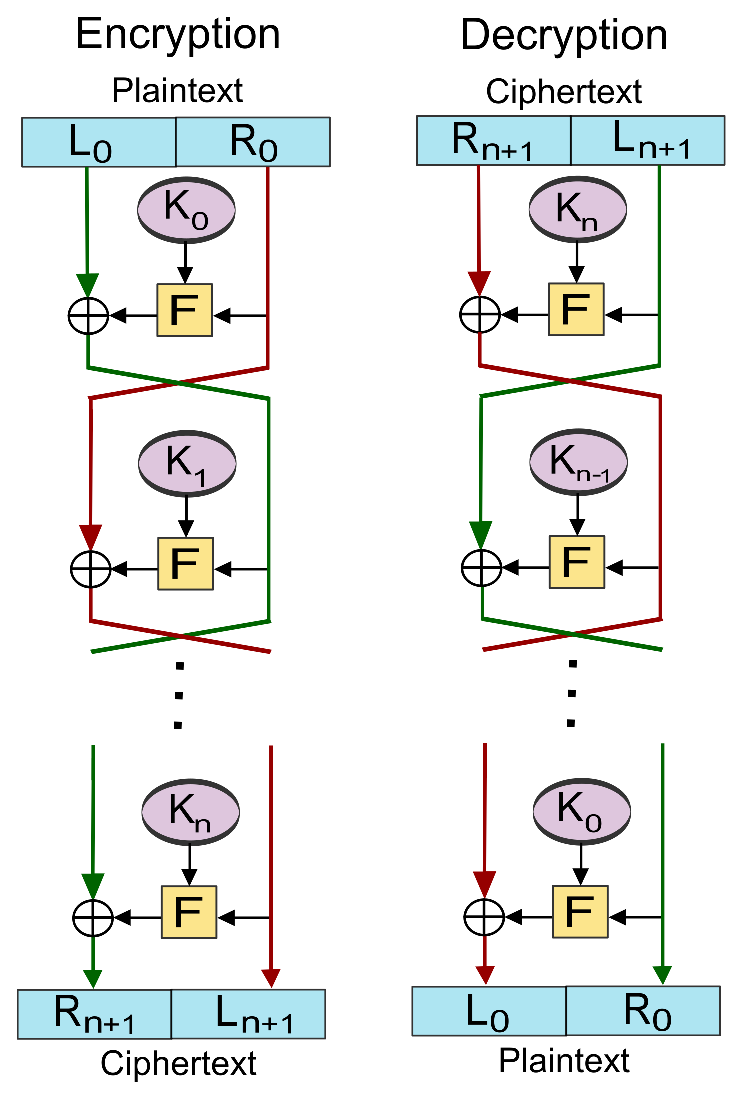
\includegraphics[scale=0.8]{chapters/chapter_3/Feistel.eps}
\end{figure}

值得注意到的一点是,在最后一次输出的时候,不再进行交换,也就是说,输出的并不是$\pth{L_{n+1}, R_{n+1}}$, 而是$\pth{R_{n+1}, L_{n+1}}$.
\subsection{SP网络}
SP网络每轮接受到输入之后,首先,将输入与该轮的子密钥进行异或,然后是对输入再次分组(也就是对分过组的明文的每组内容再次进行分组),接着将每个组通过不同的S盒进行代换,代换后的结果再拼成一个新的串,经过一个P盒的置换进行输出。\par
可以通过下图形象地理解SP网络(图源wiki):
\begin{figure}[H]
    \centering
    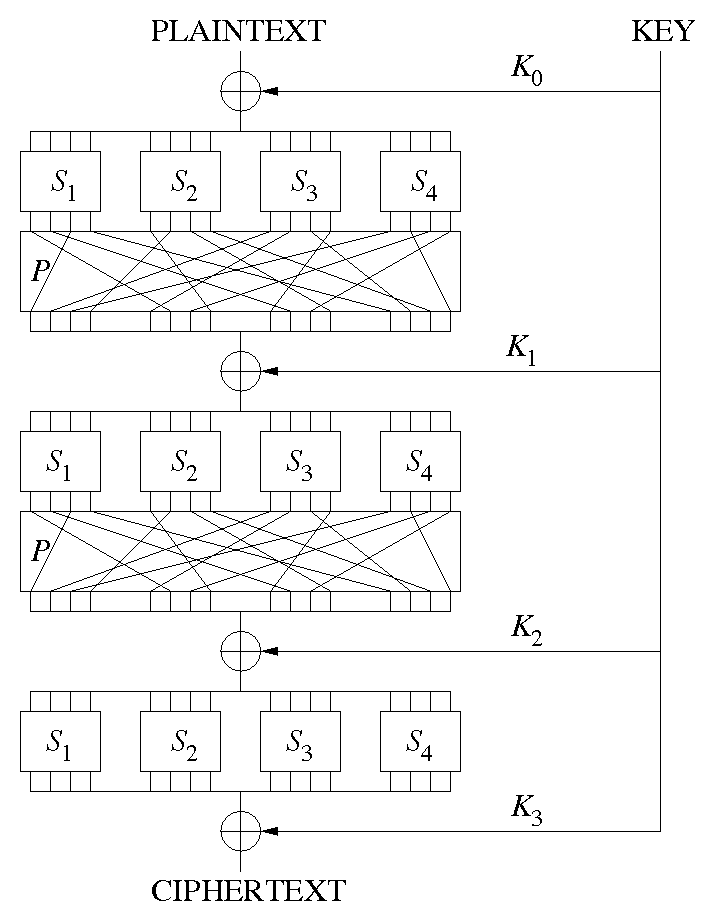
\includegraphics[scale=0.5]{chapters/chapter_3/SPN.png}
\end{figure}
\section{分组密码的运行模式}
上一节讨论了在对明文分好组后,每组内常见的加密方式。本节讨论的,则是组与组之间输入和输出的关系。在这里,假设将明文$M$分成了$m_1, m_2, \ldots, m_n$共$n$个等长的组,在每组内,加密算法为$\E{k}{m}$, 解密算法为$\D{k}{c}$.
\subsection{电码本模式(ECB)}
对于每组,其加密的输入为明文分好的组$m_i$, 密钥为同一个密钥串$k$. 也就是说,
\begin{equation}
c_i=\E{k}{m_i}
\end{equation}

其加密过程如图所示(图源wiki):
\begin{figure}[H]
\centering
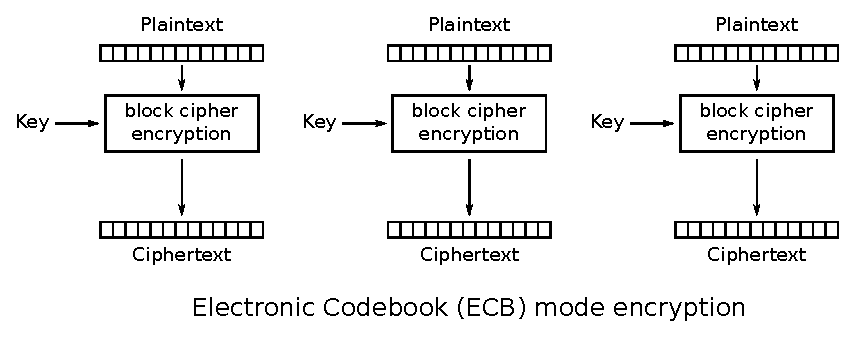
\includegraphics[scale=1]{chapters/chapter_3/ECB.eps}
\end{figure}

ECB模式极不安全。比如说,我想用ECB模式的AES密码体系加密下图:
\begin{figure}[H]
\centering
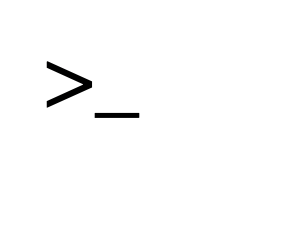
\includegraphics[scale=0.6]{chapters/chapter_3/ECB_origin.png}
\end{figure}

结果为
\begin{figure}[H]
\centering
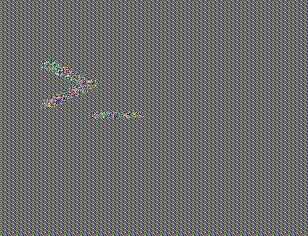
\includegraphics[scale=0.4]{chapters/chapter_3/ECB_result.jpeg}
\end{figure}
\subsection{密码分组链接模式(CBC)}
对于每组,其加密的输入为当前明文组与前一密文组的异或。也就是说,
\begin{equation}
c_i=\E{k}{m_i\oplus c_{i-1}}=\E{k}{m_i\oplus \E{k}{m_{i-1}}}
\end{equation}

对于第一组明文组,由于没有$m_0$, 因此,需要一个初始的二进制串,常记作$IV$, 来与$m_1$异或。\par
其加密过程如图所示(图源wiki):
\begin{figure}[H]
\centering
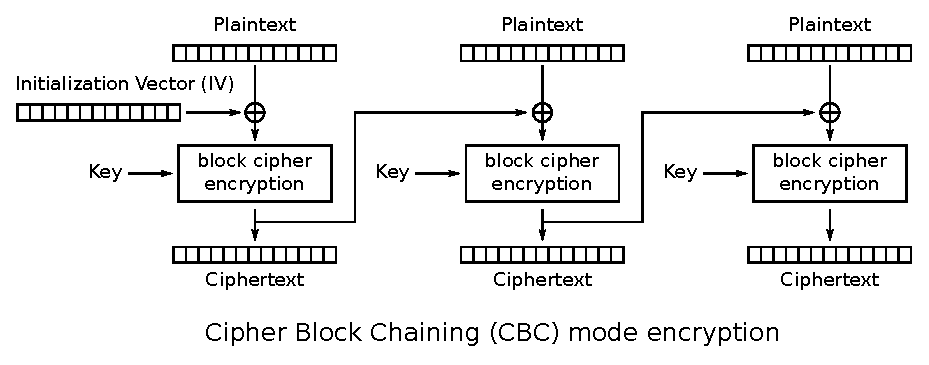
\includegraphics[scale=1]{chapters/chapter_3/CBC.eps}
\end{figure}
\subsection{密码反馈模式(CFB)}
CFB模式需要一个移位寄存器。同时,CFB模式也提供了一个可选的参数$j$, 通常取$j=8$. 其过程如下:\par
对于每组,首先需要进一步分组,使每组的长度为$j$个比特。然后对于每个新分好的组,先将移位寄存器左移$j$个比特,然后将上一组输出的$j$个比特输入到移位寄存器的右边。然后将移位寄存器内存储的二进制串用密钥$k$进行加密,其输出取前$j$个比特与本组的$j$个比特的输入进行异或输出。\par
与CBC类似,处理第一组时移位寄存器内的值也需要一组初始的二进制串$IV$.\par
因此,如果记$H_j(m)$代表取$m$的左边$j$位,$P_i$表示将每组进一步分为的$j$比特的分组,则CFB模式的加密过程可用公式描述为:
\begin{equation}
c_i=H_j\pth{\E{k}{S_{i-1}}}\oplus P_i
\end{equation}
其中$S_i$为移位寄存器的值。移位寄存器的工作方式为
\begin{equation}
S_i=\pth{\pth{S_{i-1} << x}+c_i}\bmod{64}
\end{equation}

如果忽略移位寄存器,其大致的工作原理可由下图表示(图源wiki):
\begin{figure}[H]
\centering
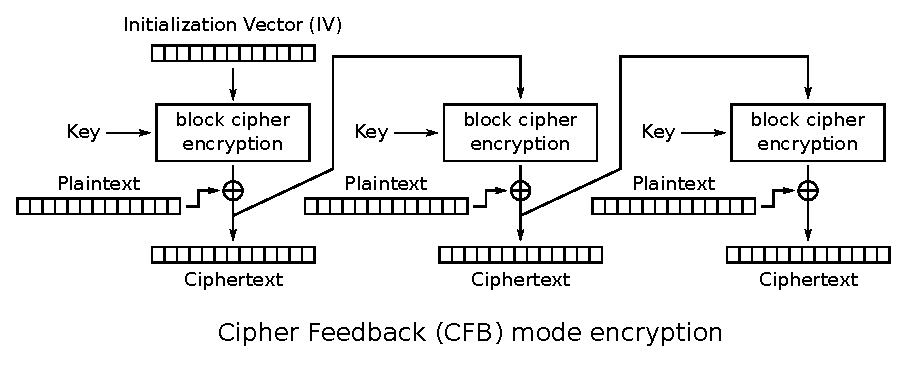
\includegraphics[scale=1]{chapters/chapter_3/CFB.eps}
\end{figure}
\subsection{输出反馈模式(OFB)}
OFB模式与CFB模式极其类似,区别仅在于每组向移位寄存器内的输入为上一组内与明文异或之前的输出。如下图所示(图源wiki):
\begin{figure}[H]
\centering
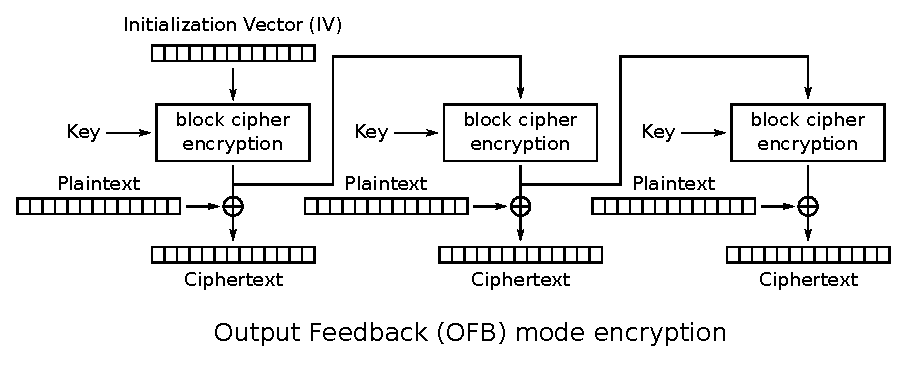
\includegraphics[scale=1]{chapters/chapter_3/OFB.eps}
\end{figure}

从图中可以看到,每组之间传递的数据与明文无关。因此,在OFB中,明文出错只会影响该组的密文,之后的密文都不会被影响。
\subsection{计数器模式(CTR)}
在借鉴了OFB中本组明文不参与下一组加密的经验之后,引入了CTR模式。在CTR模式中,存在一个计数器函数$f$. 其接受一个初始值,并在每组加密完成后,进行计数,累加到初始值之上。然后每组加密的时候,只需要将该函数的返回值输入分组加密算法中,输出值与当前明文组异或产生密文输出。\par
其过程如图所示(图源wiki):
\begin{figure}[H]
\centering
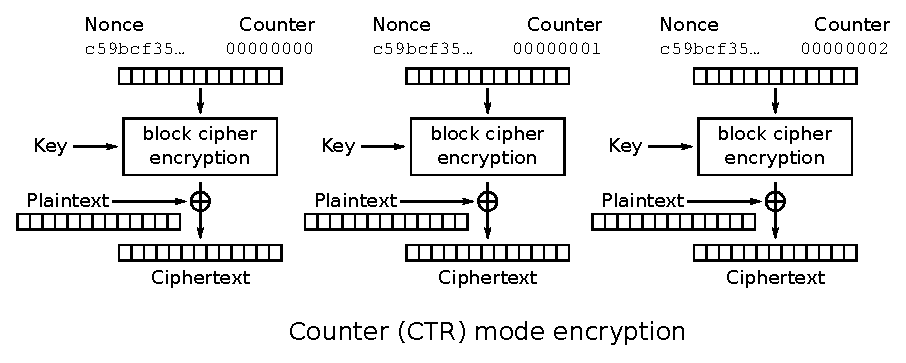
\includegraphics[scale=1]{chapters/chapter_3/CTR.eps}
\end{figure}

根据上图,我们可以发现CTR的独一无二的好处:可以并行加密。其每组加密不需要上组的任何信息,只需要该组对应的计数器值即可。
\section{DES}
接下来,我们讨论的是,在每组内的分组加密算法。\par
DES是最著名的分组密码之一。我们可以先大致地讨论其算法,然后再讨论其一些性质。
\subsection{算法与代码}
DES采用了费斯妥密码的结构,并对它进行了一定的改进。之前我们提到的费斯妥密码,可以改进的地方有其最开始的输入、子密钥、轮函数以及最后的输出。因此,我们分别就上述几个方面来分块解释DES的算法。
\subsubsection{主体:费斯妥密码}
首先,我们介绍DES的主体——费斯妥密码。正如之前说的,费斯妥密码为一个步骤的多轮操作。其核心公式为
\begin{gather}
    L_{i}=R_{i-1}\\
    R_{i}=L_{i-1}\oplus F\pth{R_{i-1}, K_i}
\end{gather}
其中,$L_{i-1}, R_{i-1}$为上一轮输出的左右两半,$L_i, R_i$为本轮输出的左右两半,$F\pth{R_{i-1}, K_i}$为轮函数,$K_i$为本轮的子密钥。\par
此外,从数学上可以证明,费斯妥密码的解密过程的核心公式也是上述公式,只不过使用的密钥的顺序与加密正好相反。\par
DES密码一共进行16轮这样的步骤,并且其输入为64位二进制串,子密钥为48位二进制串,输出为64位二进制串。\par
其C程序代码如下:
\begin{prove}
\begin{verbatim}
bitset<64> round(bitset<64> input, bitset<48> ki)
{
    bitset<64> output;
    bitset<32> previousLeftPart;
    bitset<32> leftPart;
    bitset<32> rightPart;
    
    for (int i = 0; i < 32; i++)
        previousLeftPart[31 - i] = input[63 - i];
    
    for (int i = 0; i < 32; i++)
        leftPart[31 - i] = input[31 - i];
    
    rightPart = previousLeftPart ^ F(leftPart, ki);
    
    for (int i = 0; i < 32; i++)
        output[63 - i] = leftPart[31 - i];
    
    for (int i = 32; i < 64; i++)
        output[63 - i] = rightPart[63 - i];

    return output;
}
\end{verbatim}
\end{prove}
\subsubsection{费斯妥密码的轮函数}
在费斯妥密码的轮函数这里,实际上是采用了SP网络的思想,也就是将轮函数的输入经过S盒的代换来混淆和P盒的置换来扩散。\par
轮函数接受32位的输入和48位的子密钥。首先,将32位的输入扩充成48位的二进制串(可以理解成通过了一个32位到48位的S盒,称为选择扩展运算E),然后将其逐比特与48位的子密钥异或,输出的48位二进制串作为一个48位到32位的S盒的输入。接着,将S盒输出的32位二进制串经过一个P盒(称为置换运算P)输出。\par
这里的48位到32位的S盒实际上是由8个6位到4位的S盒组成。其将输入的48位分组输入,然后再分组输出。\par
因此,轮函数所做的事情有:将32位的输入扩展成48位,进行异或,输入S盒,输入P盒。其C程序代码如下:
\begin{prove}
    \begin{verbatim}
int E[] = {32,  1,  2,  3,  4,  5,
            4,  5,  6,  7,  8,  9,
            8,  9, 10, 11, 12, 13,
           12, 13, 14, 15, 16, 17,
           16, 17, 18, 19, 20, 21,
           20, 21, 22, 23, 24, 25,
           24, 25, 26, 27, 28, 29,
           28, 29, 30, 31, 32,  1};

int S_BOX[8][4][16] = {
    {
        {14,4,13,1,2,15,11,8,3,10,6,12,5,9,0,7},
        {0,15,7,4,14,2,13,1,10,6,12,11,9,5,3,8},
        {4,1,14,8,13,6,2,11,15,12,9,7,3,10,5,0},
        {15,12,8,2,4,9,1,7,5,11,3,14,10,0,6,13}
    },
    {
        {15,1,8,14,6,11,3,4,9,7,2,13,12,0,5,10},
        {3,13,4,7,15,2,8,14,12,0,1,10,6,9,11,5},
        {0,14,7,11,10,4,13,1,5,8,12,6,9,3,2,15},
        {13,8,10,1,3,15,4,2,11,6,7,12,0,5,14,9}
    },
    {
        {10,0,9,14,6,3,15,5,1,13,12,7,11,4,2,8},
        {13,7,0,9,3,4,6,10,2,8,5,14,12,11,15,1},
        {13,6,4,9,8,15,3,0,11,1,2,12,5,10,14,7},
        {1,10,13,0,6,9,8,7,4,15,14,3,11,5,2,12}
    },
    {
        {7,13,14,3,0,6,9,10,1,2,8,5,11,12,4,15},
        {13,8,11,5,6,15,0,3,4,7,2,12,1,10,14,9},
        {10,6,9,0,12,11,7,13,15,1,3,14,5,2,8,4},
        {3,15,0,6,10,1,13,8,9,4,5,11,12,7,2,14}
    },
    {
        {2,12,4,1,7,10,11,6,8,5,3,15,13,0,14,9},
        {14,11,2,12,4,7,13,1,5,0,15,10,3,9,8,6},
        {4,2,1,11,10,13,7,8,15,9,12,5,6,3,0,14},
        {11,8,12,7,1,14,2,13,6,15,0,9,10,4,5,3}
    },
    {
        {12,1,10,15,9,2,6,8,0,13,3,4,14,7,5,11},
        {10,15,4,2,7,12,9,5,6,1,13,14,0,11,3,8},
        {9,14,15,5,2,8,12,3,7,0,4,10,1,13,11,6},
        {4,3,2,12,9,5,15,10,11,14,1,7,6,0,8,13}
    },
    {
        {4,11,2,14,15,0,8,13,3,12,9,7,5,10,6,1},
        {13,0,11,7,4,9,1,10,14,3,5,12,2,15,8,6},
        {1,4,11,13,12,3,7,14,10,15,6,8,0,5,9,2},
        {6,11,13,8,1,4,10,7,9,5,0,15,14,2,3,12}
    },
    {
        {13,2,8,4,6,15,11,1,10,9,3,14,5,0,12,7},
        {1,15,13,8,10,3,7,4,12,5,6,11,0,14,9,2},
        {7,11,4,1,9,12,14,2,0,6,10,13,15,3,5,8},
        {2,1,14,7,4,10,8,13,15,12,9,0,3,5,6,11}
    }
};

int P[] = {16,  7, 20, 21,
           29, 12, 28, 17,
            1, 15, 23, 26,
            5, 18, 31, 10,
            2,  8, 24, 14,
           32, 27,  3,  9,
           19, 13, 30,  6,
           22, 11,  4, 25};

bitset<4> S_boxi(bitset<6> input, int i)
{
    int row = 2 * input[5] + input[0];
    int column = 8 * input[4] + 4 * input[3] + 2 * input[2]
                 + input[1];
    int outputint = S_BOX[i][row][column];
    bitset<4> output(outputint);

    return output;
}
           
bitset<32> S_box(bitset<48> input)
{
    bitset<32> output;
    bitset<6> SiInput[8];

    for (int i = 0; i < 8; i++)
    {
        for (int j = 0; j < 6; j++)
            SiInput[i][5 - j] = input[47 - (j + i * 6)];

        bitset<4> SiOutput = S_boxi(SiInput[i], i);

        for (int j = 0; j < 4; j++)
            output[31 - (j + i * 4)] = SiOutput[3 - j];
    }

    return output;
}
           
bitset<32> F(bitset<32> rightPart, bitset<48> ki)
{
    bitset<32> output;
    bitset<48> expandedInput;

    for (int i = 0; i < 48; i++)
        expandedInput[47 - i] = rightPart[32 - E[i]];

    bitset<48> S_boxInput = expandedInput ^ ki;
    bitset<32> S_boxOutput = S_box(S_boxInput);

    for (int i = 0; i < 32; i++)
        output[31 - i] = S_boxOutput[32 - P[i]];

    return output;
}
    \end{verbatim}
\end{prove}
\subsubsection{费斯妥密码的最初输入}
DES加密算法接受64位明文输入,DES解密算法接受64位密文输入。为了更好地实现扩散性,首先,需要将输入的64位二进制串经过一个P盒。在DES算法中,这个P盒被称作初始置换IP. 随后,将经过置换后的64位二进制串作为费斯妥密码的输入。\par
其C程序代码如下:
\begin{prove}
    \begin{verbatim}
int IP[] = {58, 50, 42, 34, 26, 18, 10, 2,
            60, 52, 44, 36, 28, 20, 12, 4,
            62, 54, 46, 38, 30, 22, 14, 6,
            64, 56, 48, 40, 32, 24, 16, 8,
            57, 49, 41, 33, 25, 17, 9,  1,
            59, 51, 43, 35, 27, 19, 11, 3,
            61, 53, 45, 37, 29, 21, 13, 5,
            63, 55, 47, 39, 31, 23, 15, 7};

bitset<64> getInitialPermutation(bitset<64> input)
{
    bitset<64> initialPermutation;

    for (int i = 0; i < 64; i++)
        initialPermutation[63 - i] = input[64 - IP[i]];

    return initialPermutation;
}
    \end{verbatim}
\end{prove}
\subsubsection{费斯妥密码的最终输出}
之前我们再三强调,费斯妥密码的最后一轮输出后,还要将左右两边互换,也就是最终输出为$\pth{R_{16}, L_{16}}$而非$\pth{L_{16}, R_{16}}$. 此外,为了使DES的加密和解密算法能尽可能复用,我们将输出再经过一个P盒才形成最终的DES的输出。其中,输出时经过的P盒要是输入时P盒的逆,被称为逆初始置换$\mathrm{IP}^{-1}$. 这样的话,我们假设明文为$m$, 密文为$c$, 中间的费斯妥密码部分(包括最后的左右交换),加密为$f(x)$, 解密为$f^{-1}(x)$. 那么,DES加密的过程为
\[c=\mathrm{IP}^{-1}\pth{f\pth{\mathrm{IP}\pth{m}}}\]

而只需要把中间的$f$换成$f^{-1}$:
\begin{align*}
    &\mathrm{IP}^{-1}\pth{f^{-1}\pth{\mathrm{IP}\pth{c}}}\\
    =&\mathrm{IP}^{-1}\pth{f^{-1}\pth{\mathrm{IP}\pth{\mathrm{IP}^{-1}\pth{f\pth{\mathrm{IP}\pth{m}}}}}}\\
    =&\mathrm{IP}^{-1}\pth{f^{-1}\pth{f\pth{\mathrm{IP}\pth{m}}}}\\
    =&\mathrm{IP}^{-1}\pth{\mathrm{IP}\pth{m}}\\
    =&m
\end{align*}
即可实现解密。\par
因此,DES输出包括交换费斯妥密码输出的左右位置,以及通过逆初始置换$\mathrm{IP}^{-1}$. 其C程序代码如下:
\begin{prove}
    \begin{verbatim}
int IP_1[] = {40, 8, 48, 16, 56, 24, 64, 32,
              39, 7, 47, 15, 55, 23, 63, 31,
              38, 6, 46, 14, 54, 22, 62, 30,
              37, 5, 45, 13, 53, 21, 61, 29,
              36, 4, 44, 12, 52, 20, 60, 28,
              35, 3, 43, 11, 51, 19, 59, 27,
              34, 2, 42, 10, 50, 18, 58, 26,
              33, 1, 41,  9, 49, 17, 57, 25};

bitset<64> exchangeLeftAndRight(bitset<64> input)
{
    bitset<64> output;

    for (int i = 0; i < 32; i++)
        output[63 - i] = input[31 - i];

    for (int i = 32; i < 64; i++)
        output[63 - i] = input[95 - i];

    return output;
}

bitset<64> getInversePermutation(bitset<64> input)
{
    bitset<64> output;

    for (int i = 0; i < 64; i++)
        output[63 - i] = input[64 - IP_1[i]];

    return output;
}
    \end{verbatim}
\end{prove}
\subsubsection{密钥的处理}
对于输入的密钥,我们需要让其生成16个子密钥。类似于费斯妥密码,这里的16次生成也是同样的步骤循环16次。但首先,我们需要处理的是DES算法输入的64位密钥。\par
DES算法输入的64位密钥中,通常包含8位奇偶校验位。首先,我们将奇偶校验位去除,得到56位的真正的密钥。然后,再将其通过一个P盒(称为置换选择1:PC\_1),作为接下来生成子密钥的算法的输入。\par
其C程序代码为:
\begin{prove}
\begin{verbatim}
int PC_1[] = {57, 49, 41, 33, 25, 17, 9,
               1, 58, 50, 42, 34, 26, 18,
              10,  2, 59, 51, 43, 35, 27,
              19, 11,  3, 60, 52, 44, 36,
              63, 55, 47, 39, 31, 23, 15,
               7, 62, 54, 46, 38, 30, 22,
              14,  6, 61, 53, 45, 37, 29,
              21, 13,  5, 28, 20, 12,  4};

bitset<56> getKeyPermutation(bitset<64> key)
{
    bitset<56> output;

    for (int i = 0; i < 56; i++)
        output[55 - i] = key[64 - PC_1[i]];

    return output;
}
\end{verbatim}
\end{prove}
\subsubsection{子密钥的生成}
由于DES算法中的费斯妥密码部分一共需要16轮循环,因此共需要16个子密钥。在DES算法中,采用了同一个步骤循环16次的方式生成子密钥。该步骤接受56位二进制串的输入,生成48位的子密钥和56位的输出。其包含两个操作:循环移位和置换选择2。\par
之前我们提到,在DES密码算法中,加密和解密仅有的区别就是子密钥的使用顺序。因此,这种区别就体现在了子密钥生成的算法上。\par
在循环移位步骤中,其接受56位的输入,然后将这56位的二进制串分为左右两个28位的二进制串。并在每一轮中,将这两个二进制串分别循环移位。加密过程是左循环移位,解密过程是右循环移位,并且每一轮移动的位数不同。\par
在循环移位操作完成后,将左右两个二进制串重新拼成一个56位的二进制串作为输出和下一轮操作的输入,同时,再将56位的二进制串经过一个56位到48位的S盒(称为置换选择2: PC\_2), 作为本轮的子密钥。\par
其C程序代码为:
\begin{prove}
\begin{verbatim}
enum ShiftStyle {
    leftShift,
    rightShift
};

int shiftBits[] = {1, 1, 2, 2, 2, 2, 2, 2, 1, 2, 2, 2, 2, 
                    2, 2, 1};
int inverseShiftBits[] = {0, 1, 2, 2, 2, 2, 2, 2, 1, 2, 2, 
                            2, 2, 2, 2, 1};

int PC_2[] = {14, 17, 11, 24,  1,  5,
               3, 28, 15,  6, 21, 10,
              23, 19, 12,  4, 26,  8,
              16,  7, 27, 20, 13,  2,
              41, 52, 31, 37, 47, 55,
              30, 40, 51, 45, 33, 48,
              44, 49, 39, 56, 34, 53,
              46, 42, 50, 36, 29, 32};

bitset<56> shiftKey(bitset<56> key, int round, 
                    ShiftStyle shiftStyle)
{
    bitset<56> output;

    bitset<28> previousLeftPart;
    for (int i = 0; i < 28; i++)
        previousLeftPart[27 - i] = key[55 - i];

    bitset<28> previousRightPart;
    for (int i = 0; i < 28; i++)
        previousRightPart[27 - i] = key[27 - i];

    int *shift;
    switch (shiftStyle)
    {
        case leftShift:
            shift = shiftBits;
            break;
            
        case rightShift:
            shift = inverseShiftBits;
            break;
            
        default:
            break;
    }
    
    bitset<28> leftPart;
    bitset<28> rightPart;
    int shiftBit = shift[round];

    switch (shiftStyle)
    {
        case leftShift:
            for (int i = 0; i < 28; i++)
            {
                leftPart[27 - i] = previousLeftPart[(27 - i
                                     - shiftBit + 28) % 28];
                rightPart[27 - i] = previousRightPart[(27 - i
                                     - shiftBit + 28) % 28];
            }
            break;
            
        case rightShift:
            for (int i = 0; i < 28; i++)
            {
                leftPart[27 - i] = previousLeftPart[(27 - i
                                     + shiftBit + 28) % 28];
                rightPart[27 - i] = previousRightPart[(27 - i
                                     + shiftBit + 28) % 28];
            }
            break;
            
        default:
            break;
    }

    for (int i = 0; i < 28; i++)
        output[55 - i] = leftPart[27 - i];

    for (int i = 28; i < 56; i++)
        output[55 - i] = rightPart[55 - i];

    return output;
}

bitset<48> getSubkey(bitset<56> key, int round, 
                     ShiftStyle shiftStyle)
{
    bitset<48> output;

    for (int i = 0; i < 48; i++)
        output[47 - i] = key[56 - PC_2[i]];

    return output;
}
\end{verbatim}
\end{prove}
\subsubsection{DES加密和解密}
以上就是DES密码的每个组成部分。我们可以把它们组合起来,实现DES的加密和解密。其C程序代码如下:
\begin{prove}
\begin{verbatim}
bitset<64> DES_ENC(bitset<64> plainText, bitset<64> key)
{
    bitset<64> cipher;
    bitset<64> roundInput = getInitialPermutation(plainText);
    bitset<64> roundOutput;
    bitset<56> permutatedKey = getKeyPermutation(key);
    bitset<56> previousShiftOutput = shiftKey(permutatedKey, 0,
                                                 leftShift);
    for (int i = 0; i < 16; i++)
    {
        bitset<48> subkey = getSubkey(previousShiftOutput, i, 
                                        leftShift);
        roundOutput = round(roundInput, subkey);
        roundInput = roundOutput;
        previousShiftOutput = shiftKey(previousShiftOutput, 
                                        i + 1, leftShift);
    }
    cipher = getInversePermutation(
                exchangeLeftAndRight(roundOutput));
    return cipher;
}

bitset<64> DES_DEC(bitset<64> cipher, bitset<64> key)
{
    bitset<64> plainText;
    bitset<64> roundInput = getInitialPermutation(cipher);
    bitset<64> roundOutput;
    bitset<56> permutatedKey = getKeyPermutation(key);
    bitset<56> previousShiftOutput = shiftKey(permutatedKey, 0, 
                                                rightShift);
    for (int i = 0; i < 16; i++)
    {
        bitset<48> subkey = getSubkey(previousShiftOutput, i, 
                                        rightShift);
        roundOutput = round(roundInput, subkey);
        roundInput = roundOutput;
        previousShiftOutput = shiftKey(previousShiftOutput, 
                                        i + 1, rightShift);
    }
    plainText = getInversePermutation(
                    exchangeLeftAndRight(roundOutput));
    return plainText;
}
\end{verbatim}
\end{prove}
\subsection{多重DES}
我们可以看出,DES密码使用了费斯妥密码,并且局部也使用了SP网络,这样使这种分组密码的安全性较高。在几乎30年的大量研究之后,已知对DES的最好的实用攻击仍然只是对密钥空间的穷举搜索。但是,DES使用的密钥在去除奇偶校验位之后的实际长度只有56位,在如今的计算机水平下,变得十分容易破解。在2017年,通过计算机更是创下了在25秒内破解DES的记录。\par
鉴于此,人们选择了多重DES加密。如二重DES加密:使用一个112位的密钥$K$, 将其分为$K_1$和$K_2$两个56位的密钥。如果记$\mathrm{E}_k\pth{m}$为DES的加密过程,$\mathrm{D}_k\pth{m}$为DES的解密过程,那么,其加密过程为
\[\mathrm{E}_{K_1}\pth{\mathrm{E}_{K_2}\pth{m}}\]
解密过程为
\[\mathrm{D}_{K_2}\pth{\mathrm{D}_{K_1}\pth{c}}\]

而如今最常用的是二密钥的三重DES,简称为3DES密码。其使用一个112位的密钥$K$, 将其分为$K_1$和$K_2$两个56位的密钥,其加密过程为
\[\mathrm{E}_{K_1}\pth{\mathrm{D}_{K_2}\pth{\mathrm{E}_{K_1}\pth{m}}}\]
解密过程为
\[\mathrm{D}_{K_1}\pth{\mathrm{E}_{K_2}\pth{\mathrm{D}_{K_1}\pth{c}}}\]
\subsection{结构特性}
除了DES的密钥过短,从数学角度来看,DES密码拥有一些结构特性,也降低了其破解的难度。
\subsubsection{互补特性}
对于二进制串$m$, 如果我们记$\overline{m}$为$m$按位取补,并用$\mathrm{DES}_k\pth{m}$表示通过密钥$k$, 二进制串$m$的DES加密的密文,那么,我们可以证明:
\begin{equation}
\mathrm{DES}_{\overline{k}}\pth{\overline{m}}=\overline{\mathrm{DES}_k\pth{m}}
\end{equation}

因此,在使用穷举搜索破解时,可以使工作量减少一半。假设有一个使用已知明文攻击的攻击者,他可以选择明密文对$\pth{M, C}$和$\pth{\overline{M}, C^*}$. 那么,在所有的$2^{56}$个可能的密钥,也就是$2^{55}$对互补的密钥二进制串中,他只需要每对互补的二进制串中取一个,一共搜索$2^{55}$个密钥。对于每个尝试的密钥$l$, 如果$\mathrm{DES}_{l}\pth{M}=C$或$\overline{C^*}$, 就说明密钥是$l$或$\overline{l}$.
\subsubsection{弱密钥与半弱密钥}
在多重DES加密的过程中,有一些密钥十分危险。比如说弱密钥:
\begin{Definition}
在DES加密的过程中,如果存在一个密钥$w$, 使得
\begin{equation}\label{weakKey}
\mathrm{E}_w\pth{\mathrm{E}_w\pth{m}}=m
\end{equation}

则称$w$为弱密钥。
\end{Definition}

从另一个角度解释公式\ref{weakKey}, 也就是说,
\begin{equation}
\mathrm{E}_w\pth{m}=\mathrm{D}_w\pth{m}
\end{equation}

而我们之前提到,DES密码的加密与解密过程唯一的区别就是子密钥的使用顺序。据此我们可以很容易地构造弱密钥$w$, 也就是使其生成子密钥时加密与解密循环移位的结果相同即可。在56位的密钥中,共有4个弱密钥。\par
此外,还有半弱密钥对
\begin{Definition}
在DES加密的过程中,如果存在一对密钥$w_1, w_2$, 使得
\begin{equation}
\mathrm{E}_{w_1}\pth{\mathrm{E}_{w_2}\pth{m}}=m
\end{equation}

则称$w_1, w_2$为一对半弱密钥。
\end{Definition}

在3DES密码中,如果选取的两个密钥是一对半弱密钥,后果不堪设想。在56位的密钥中,共有6对半弱密钥。
\section{IDEA}
\subsection{符号说明}
在介绍IDEA之前,首先,先介绍一些IDEA加密过程中用到的数学符号。
\begin{itemize}
\item 逐比特异或$\oplus$\par
$m_1\oplus m_2$即将两个16位的二进制串逐比特异或。
\item 模$2^{16}$整数加法$\boxplus$\par
即对于16位二进制数$m_1, m_2$, $m_1\boxplus m_2=\pth{m_1+m_2}\bmod{2^{16}}$.
\item 模$2^{16}+1$整数乘法$\odot$\par
即对于16为二进制数$m_1, m_2$, $m_1\odot m_2=\pth{m_1\cdot m_2}\bmod{\pth{2^{16}+1}}$.\par
这里特别指出,如果$m_1=00\ldots 0$, 应把$m_1$看作$2^{16}$. 这是由于$2^{16}+1=65537$为素数,故由数论知识我们可以知道,模$2^{16}+1$的非零整数乘法构成一个群,即所有非零整数都有逆元。此外,这样也可以保证输出一定不会超过16位。由于$2^{16}+1$为素数,所以如果$\pth{m_1m_2}\bmod{\pth{2^{16}+1}}=0$, 则表明$m_1$或$m_2$必然是$2^{16}+1$的倍数。而$m_1, m_2$均为16位字符串,所以这是不可能的。
\end{itemize}
\subsection{轮结构}
和其他分组密码类似,IDEA也是采用了多次重复轮结构的步骤。其轮结构如图所示(图源wiki):
\begin{figure}[H]
\centering
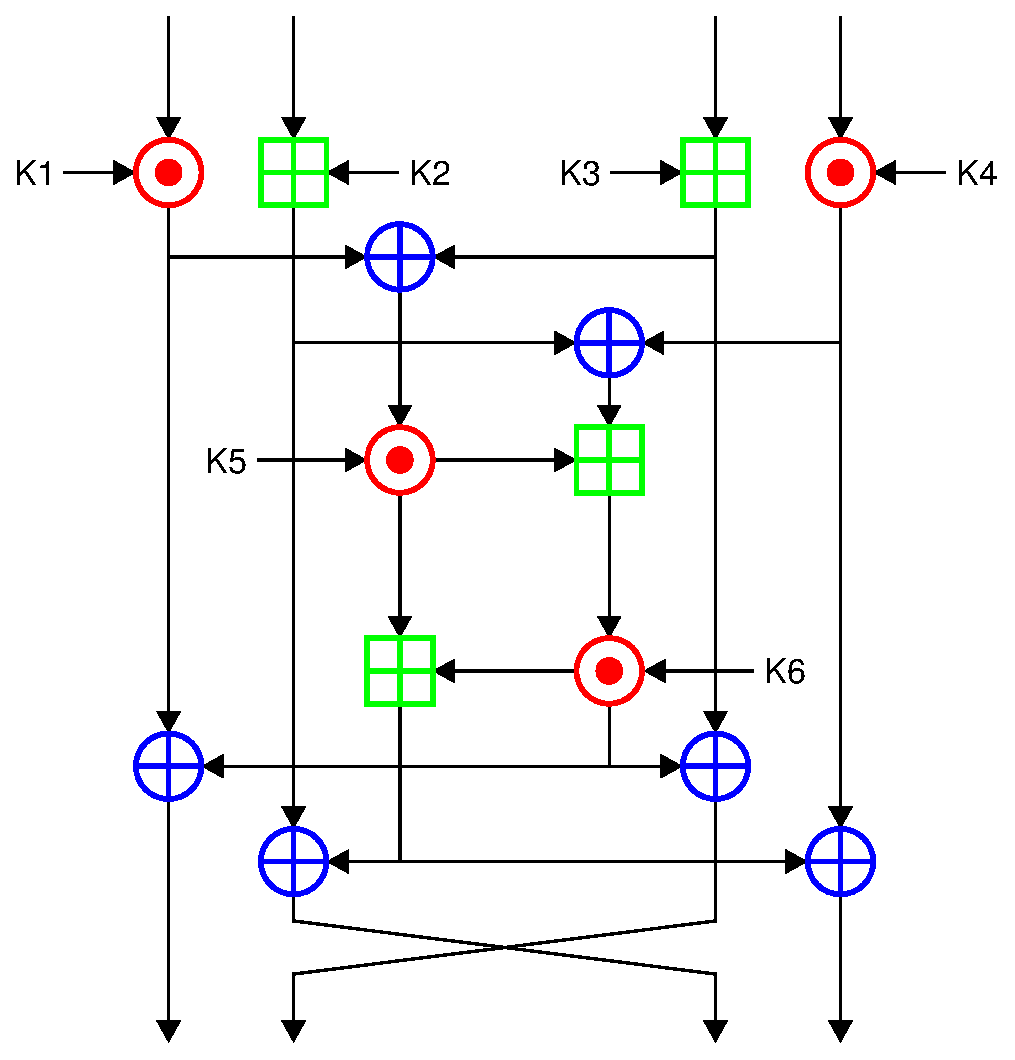
\includegraphics[scale=0.5]{chapters/chapter_3/IDEA_round.eps}
\end{figure}

在每一轮中,一共需要输入6个16位的子密钥,并且输入为4组16位的二进制串,输出也为4组16位的二进制串。
\subsection{加密过程}
IDEA加密算法接受64位明文和128位密钥。对于密钥,将其通过一个子密钥生成器生成48个16位的子密钥用于8轮轮结构,加上6个16位的子密钥用于输出变换。\par
首先,将64位明文分成4组等长的子串,然后输入轮结构中。在经过8轮轮结构后,将输出的结构通过如图所示的输出变换(图源wiki),得到密文。
\begin{figure}[H]
\centering
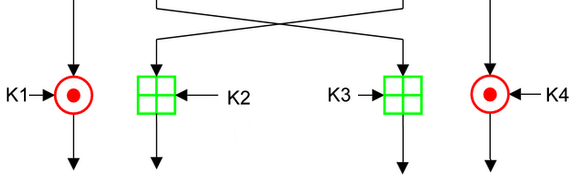
\includegraphics[scale=0.5]{chapters/chapter_3/IDEA_output.png}
\end{figure}

而子密钥的生成算法则相对比较直接:\par
前8个子密钥$Z_1, Z_2, \ldots, Z_8$直接在加密密钥中依次选取。然后,将加密密钥循环左移$52$位,再依次取接下来的8个子密钥。以此类推,直到52个子密钥全部生成。
\section{AES}
\subsection{输入与输出}
AES密码接受的明文与密钥的长度可独立选择128位、192位或256位。这些选择之间的区别仅仅在于加密运算的轮数以及子密钥的调度不同。但是在AES密码标准中,明文长度固定为128位,密钥长度可以选择为128, 192或256位,分别叫做AES-128, AES-192和AES-256.\par
在处理过程中,我们对明文和密钥进一步分组。AES密码的每个步骤的处理单位是一个“字节”,即8个比特。因此,我们将明文和密钥分成每组长度为8比特的分组,每个8比特的明文分组称为一个“状态”。\par
对于由字节组成的明文,我们第二次进行分组,使其分成4个等长的分组,记明文的每个分组的长度为$N_b$ (在实际操作中明文总是128位,因此$N_b=4$). 此外,我们也记以字节为单位的密钥的长度除以$4$为$N_k$ ($N_k$的可能取值为$4, 6, 8$). 我们如果假定由字节组成的明文是一个长度为$4N_b$的数列$\{M_n\}$, 那么,我们可以按下表的顺序填充分组:
\begin{table}[H]
\centering
\begin{tabular}{c|c|c|c}\hline
$M_0$&$M_4$&$\cdots$&$M_{4N_b-3}$\\\hline
$M_1$&$M_5$&$\cdots$&$M_{4N_b-2}$\\\hline
$M_3$&$M_6$&$\cdots$&$M_{4N_b-1}$\\\hline
$M_4$&$M_7$&$\cdots$&$M_{4N_b}$\\\hline
\end{tabular}
\end{table}

由明文的分组组成的阵列称为状态阵列。在AES的实际过程中,都是对状态阵列进行操作。最终的密文就是从状态序列中,按写入顺序拿出的序列。\par
因此,在加密的输入阶段,我们要做的事是将明文和密钥按字节分组,然后将明文再填入状态阵列中。在加密的输出阶段,就是将密文从状态阵列中读出,再变成以比特为单位的二进制串(但事实上,明文或密文的按字节分组可以直接在填入状态阵列的时候做。因此,我们只需要实现比特串向字节串的转化用于密钥,而不需要实现字节串向比特串的转化)。在解密阶段,我们要做的也是同样的步骤,只不过是明文和密文对调。\par
此环节的C程序代码如下:
\begin{prove}
\begin{verbatim}
void bitToByte(bitset<128> inputBits, bitset<8> outputBytes[64])
{
    for (int byte = 0; byte < 64; byte++)
        for (int bit = 0; bit < 8; bit++)
            outputBytes[byte][bit] = inputBits[8 * byte + bit];
}

void bitToState(bitset<128> input, bitset<8> state[4][4])
{
    for (int column = 0; column < 4; column++)
        for (int row = 0; row < 4; row++)
            for (int bit = 0; bit < 8; bit++)
                state[row][column][bit] = input[32 * column
                                                + 8 * row + bit];
}

void stateToBit(bitset<8> state[4][4], bitset<128> &output)
{
    for (int column = 0; column < 4; column++)
        for (int row = 0; row < 4; row++)
            for (int bit = 0; bit < 8; bit++)
                output[32 * column + 8 * row + bit]
                    = state[row][column][bit];
}
\end{verbatim}
\end{prove}
\subsection{轮函数}
AES的轮函数由4个计算部件组成,分别为字节代换(ByteSub), 行移位(ShiftRow), 列混合(MixColumn), 密钥加(AddRoundKey).
\subsubsection{字节代换}
字节代换可以看作一个128位到128位的S盒。其接受输入状态阵列,然后对状态阵列实现S盒的操作。\par
在C程序实现里,加密过程中,S盒为\verb`bitset<8> S_box[16][16]`; 解密过程中,S盒为\verb`bitset<8> Inv_S_Box[16][16]`. 这两个S盒的值在AES中是固定的,其生成方式可以看后面的数学论证部分。\par
其C程序实现如下:
\begin{prove}
\begin{verbatim}
void SubByte(bitset<8> state[4][4], CryptoMode cryptoMode)
{
    bitset<8> (*crypto_S_box)[16];

    switch (cryptoMode)
    {
        case Enc:
            crypto_S_box = S_box;
            break;
            
        case Dec:
            crypto_S_box = Inv_S_Box;
            break;
            
        default:
            break;
    }
    
    for (int row = 0; row < 4; row++)
        for (int column = 0; column < 4; column++)
        {
            bitset<8> previousValue = *(*(state + row) + column);
            int S_box_row = previousValue[7] * 8
                                + previousValue[6] * 4
                                    + previousValue[5] * 2
                                        + previousValue[4];
            int S_box_column = previousValue[3] * 8
                                + previousValue[2] * 4
                                    + previousValue[1] * 2
                                        + previousValue[0];
            *(*(state + row) + column)
                = crypto_S_box[S_box_row][S_box_column];
        }
}
\end{verbatim}
\end{prove}
\subsubsection{行移位}
在之前处理数据的时候,我们提到把明文分为4组。每组可以看作一行,每行包括$N_b$个字节。\par
所谓行移位,就是将各行进行循环移位,不同的行的位移量不同。第一行不移位,第二行左移$C_1$, 第三行左移$C_2$, 第四行左移$C_3$. $C_1, C_2, C_3$都与$N_b$有关。\par
在解密时,只需要反向循环移位即可。\par
其C程序实现如下:
\begin{prove}
\begin{verbatim}
int shiftBytes[4] = {0, 1, 2, 3};

void ShiftRows(bitset<8> state[4][4], CryptoMode cryptoMode)
{
    for (int row = 0; row < 4; row++)
    {
        bitset<8> previousRow[4];
        for (int column = 0; column < 4; column++)
            previousRow[column] = state[row][column];
        switch (cryptoMode)
        {
            case Enc:
                for (int column = 0; column < 4; column++)
                    state[row][column]
                        = previousRow[(column
                                       - shiftBytes[row] + 4) % 4];
                break;
                
            case Dec:
                for (int column = 0; column < 4; column++)
                    state[row][column]
                        = previousRow[(column
                                       + shiftBytes[row]) % 4];
                break;
                
            default:
                break;
        }
    }
}
\end{verbatim}
\end{prove}
\subsubsection{列混合}
该步骤是对状态阵列的每一列进行变换。为了方便我们理解以及后面的数学论证,我们将这一步理解成矩阵乘法。由于每一列共有4个元素,因此,我们可以把它看作一个四维列向量$(a_0, a_1, a_2, a_3)^{\mathrm{T}}$. 其输出也为4位列向量$(b_0, b_1, b_2, b_3)^{\mathrm{T}}$.\par
在加密过程中,其计算方法为
\begin{equation}
\pth{\begin{array}{c}b_0\\b_1\\b_2\\b_3\end{array}}=\pth{\begin{array}{cccc}02&03&01&01\\01&02&03&01\\01&01&02&03\\03&01&01&02\end{array}}\pth{\begin{array}{c}a_0\\a_1\\a_2\\a_3\end{array}}
\end{equation}

在解密过程中,其计算方法为
\begin{equation}
\pth{\begin{array}{c}a_0\\a_1\\a_2\\a_3\end{array}}=\pth{\begin{array}{cccc}0e&0b&0d&09\\09&0e&0b&0d\\0d&09&0e&0b\\0b&0d&09&0e\end{array}}\pth{\begin{array}{c}b_0\\b_1\\b_2\\b_3\end{array}}
\end{equation}

这里要特别指出的是,在矩阵相乘时,每一项之间的乘法并不是我们平时用到的十进制乘法。这种乘法遵循特定的乘法表。在C程序实现中,我们发现,只需要使用与01, 02, 03, 09, 0b, 0d, 0e的乘法。因此,对于这7个数,我们各有一张长度为256的表,用于与一个字节对应的比特(共$2^8=256$种)相乘($a_0, a_1, a_2, a_3$都是一个字节)的结果。\par
其C程序实现如下:
\begin{prove}
\begin{verbatim}
bitset<8> *M[4][4] = {
    {Mul_02, Mul_03, Mul_01, Mul_01},
    {Mul_01, Mul_02, Mul_03, Mul_01},
    {Mul_01, Mul_01, Mul_02, Mul_03},
    {Mul_03, Mul_01, Mul_01, Mul_02}
};

bitset<8> *Inv_M[4][4] = {
    {Mul_0e, Mul_0b, Mul_0d, Mul_09},
    {Mul_09, Mul_0e, Mul_0b, Mul_0d},
    {Mul_0d, Mul_09, Mul_0e, Mul_0b},
    {Mul_0b, Mul_0d, Mul_09, Mul_0e}
};

void MixColumns(bitset<8> state[4][4], CryptoMode cryptoMode)
{
    bitset<8>* (*crypto_M)[4][4];

    switch (cryptoMode)
    {
        case Enc:
            crypto_M = &M;
            break;
            
        case Dec:
            crypto_M = &Inv_M;
            break;
            
        default:
            break;
    }
    for (int column = 0; column < 4; column++)
    {
        bitset<8> previousColumn[4];
        for (int row = 0; row < 4; row++)
            previousColumn[row] = state[row][column];
        for (int row = 0; row < 4; row++)
        {
            state[row][column] = 0;
            for (int i = 0; i < 4; i++)
                state[row][column]
                    ^= *(*(*(*crypto_M + row) + i)
                        + previousColumn[row].to_ulong());
        }
    }
}
\end{verbatim}
\end{prove}
\subsubsection{密钥加}
在我们输入密钥之后,首先会通过密钥编排算法,得到若干长度为$N_b$的轮密钥。密钥加即为将轮密钥与当前的状态阵列逐比特异或。解密时再次异或即可。\par
其C程序实现如下:
\begin{prove}
\begin{verbatim}
void AddRoundKey(bitset<8> state[4][4], bitset<32> ki[4])
{
    for (int row = 0; row < 4; row++)
        for (int column = 0; column < 4; column++)
            for (int bit = 0; bit < 8; bit++)
                state[row][column][bit]
                    = ki[row][column * 4 + bit]
                        ^ state[row][column][bit];
}
\end{verbatim}
\end{prove}
\subsubsection{轮函数总的步骤}
在每一轮中,对当前的状态阵列,轮函数依次进行字节代换、行移位、列混合和与当前轮密钥的密钥加,最后输出。\par
在最后一轮中,不进行列混合。
\subsection{密钥编排算法}
之前我们讲到,我们输入的密钥会通过密钥编排算法变成若干长度为$N_b$的轮密钥。密钥编排算法分为密钥扩展和轮密钥选取两个部分。\par
考虑到每个轮密钥长度都为$N_b$, 假设我们需要进行$N_r$轮,则一共需要$N_b\pth{N_r+1}$长度的密钥。因此,我们首先需要将输入的密钥扩展成对应长度的扩展密钥。\par
然后,第一轮轮密钥取扩展密钥的第一个$N_b$长度个字,第二轮轮密钥取接下来的$N_b$长度个字,以此类推。\par
\subsubsection{密钥扩展算法}
在密钥扩展算法中,我们需要用到$N_r$个轮常数\verb`Rcon`,以及一些辅助工作,如对密钥的循环移位\verb`RotWord`和对密钥的替换(使用的S盒与之前的是同一个)\verb`SubWord`. 此外,对于不同的$N_r$, 密钥扩展算法也不同。\par
这里以AES-128为例,其C程序代码如下:
\begin{prove}
\begin{verbatim}
bitset<32> Rcon[10] = {0x01000000, 0x02000000, 0x04000000,
0x08000000, 0x10000000, 0x20000000, 0x40000000, 0x80000000,
0x1b000000, 0x36000000};

bitset<32> RotWord(bitset<32> input)
{
    bitset<32> output;

    for (int i = 0; i < 32; i++)
        output[i] = input[(i - 8 + 32) % 32];

    return output;
}

bitset<32> SubWord(bitset<32> input)
{
    bitset<32> output;
    
    for (int byte = 0; byte < 4; byte++)
    {
        int row = input[8 * byte + 7] * 8
                    + input[8 * byte + 6] * 4
                        + input[8 * byte + 5] * 2
                            + input[8 * byte + 4];
        int column = input[8 * byte + 3] * 8
                        + input[8 * byte + 2] * 4
                            + input[8 * byte + 1] * 2
                                + input[8 * byte];
        bitset<8> value = S_box[row][column];
        for (int bit = 0; bit < 8; bit++)
            output[8 * byte + bit] = value[bit];
    }
    
    return output;
}

void KeyExpansion(bitset<8> *key, bitset<32> *w)
{
    int Nk = 4;
    int Nr = 10;
    
    for (int word = 0; word < Nk; word++)
        for (int byte = 0; byte < 4; byte++)
            for (int bit = 0; bit < 4; bit++)
                w[word][4 * byte + bit] = key[byte][bit];

    for (int word = Nk; word < 4 * (Nr + 1); word++)
    {
        bitset<32> tmp = w[word - 1];
        if (!word % Nk)
            tmp = SubWord(RotWord(tmp)) ^ Rcon[word / Nk];
        w[word] = w[word - Nk] ^ tmp;
    }
}
\end{verbatim}
\end{prove}
\subsection{总的加解密过程}
\subsubsection{加密过程}
首先,将明文写入状态阵列,密钥变成字节串。然后,求出扩展密钥。接着,对前4个密钥使用密钥加算法。然后,在进行10轮的字节替换、行移位、列混合、密钥加,其中最后一轮不进行列混合。最后,将此时的状态阵列读出为密文。\par
其C程序代码如下:
\begin{prove}
\begin{verbatim}
bitset<128> AES_128_ENC(bitset<128> plainText, bitset<128> key)
{
    bitset<128> cipher;
    
    bitset<8> state[4][4];
    bitToState(plainText, state);
    
    bitset<8> keys[16];
    bitToByte(key, keys);
    
    bitset<32> expanedKeys[44];
    KeyExpansion(keys, expanedKeys);
    
    bitset<32> subkeys[4];
    for (int i = 0; i < 4; i++)
        subkeys[i] = expanedKeys[i];
    AddRoundKey(state, subkeys);
    
    for (int round = 0; round < 9; round++)
    {
        SubByte(state, Enc);
        ShiftRows(state, Enc);
        MixColumns(state, Enc);
        for (int i = 0; i < 4; i++)
            subkeys[i] = expanedKeys[i + 4 + round * 4];
        AddRoundKey(state, subkeys);
    }
    
    SubByte(state, Enc);
    ShiftRows(state, Enc);
    for (int i = 0; i < 4; i++)
        subkeys[i] = expanedKeys[i + 40];
    AddRoundKey(state, subkeys);
    
    stateToBit(state, cipher);

    return cipher;
}
\end{verbatim}
\end{prove}
\subsubsection{解密算法}
首先,将密文写入状态阵列,密钥变成字节串。然后,求出扩展密钥。接着,对最后4个密钥使用密钥加算法。然后,在进行10轮的字节替换、行移位、密钥加、列混合,其中最后一轮不进行列混合。最后,将此时的状态阵列读出为明文。\par
解密与加密的区别在于:轮密钥的使用顺序恰好相反(但每一轮内的顺序是相同的)。\par
其C程序代码如下:
\begin{prove}
\begin{verbatim}
bitset<128> AES_128_DEC(bitset<128> cipher, bitset<128> key)
{
    bitset<128> plainText;
    
    bitset<8> state[4][4];
    bitToState(cipher, state);
    
    bitset<8> keys[16];
    bitToByte(key, keys);
    
    bitset<32> expanedKeys[44];
    KeyExpansion(keys, expanedKeys);
    
    bitset<32> subkeys[4];
    for (int i = 0; i < 4; i++)
        subkeys[i] = expanedKeys[40 + i];
    AddRoundKey(state, subkeys);
    
    for (int round = 0; round < 9; round++)
    {
        SubByte(state, Dec);
        ShiftRows(state, Dec);
        MixColumns(state, Dec);
        for (int i = 0; i < 4; i++)
            subkeys[i] = expanedKeys[i + 36 - round * 4];
        AddRoundKey(state, subkeys);
    }
    
    SubByte(state, Dec);
    ShiftRows(state, Dec);
    for (int i = 0; i < 4; i++)
        subkeys[i] = expanedKeys[i];
    AddRoundKey(state, subkeys);
    
    stateToBit(state, plainText);

    return plainText;
}
\end{verbatim}
\end{prove}
\subsection{数学基础}
\subsubsection{有限域$\GF\pth{2^8}$}
我们之前在讲流密码的时候提到过有限域$\GF\pth{2}$. 在这里,我们就要正式地引入域的概念:\par
所谓域,就是可交换的除环。更确切地说:
\begin{Definition}
对于集合$F$和它上面的两个运算$+, \cdot$, 如果满足如下性质:
\begin{enumerate}
    \item 加法和乘法的封闭性\par
    $\forall a, b\in F, a+b\in F, a\cdot b\in F$
    \item 加法和乘法的结合律\par
    $\forall a, b, c\in F, \pth{a+b}+c=a+\pth{b+c}, \pth{a\cdot b}\cdot c=a\cdot\pth{b\cdot c}$
    \item 加法和乘法的交换律\par
    $\forall a, b\in F, a+b=b+a, a\cdot b=b\cdot a$
    \item 乘法对加法的分配率\par
    $\forall a, b, c\in F, a\cdot\pth{b+c}=a\cdot b+a\cdot c$
    \item 加法单位元\par
    $\exists a\in F, \mathrm{s.t.}\, \forall b\in F, a+b=b+a=b$\par
    常将加法单位元$a$记作$0$
    \item 乘法单位元\par
    $\exists a\in F, \mathrm{s.t.}\, \forall b\in F\text{且}b\neq 0, a\cdot b=b\cdot a=b$\par
    常将乘法单位元$a$记作$1$
    \item 加法逆元\par
    $\forall a\in F,\exists -a\in F, \mathrm{s.t.}\, a+\pth{-a}=\pth{-a}+a=0$
    \item 乘法逆元\par
    $\forall a\in F\text{且}a\neq 0, \exists a^{-1}\in F, \mathrm{s.t.}\, a\cdot a^{-1}=a^{-1}\cdot a=0$
\end{enumerate}
则称$F$和它上面的两个运算$+, \cdot$构成一个域。
\end{Definition}

如果$F$内的元素个数有限,为$n$个,则称$F$为有限域,记作$\GF\pth{n}$. 在AES中,我们主要研究有限域$\GF\pth{2^8}$.\par
熟悉抽象代数的同学可能会知道,对于任意素数$p$和正整数$n$, 所有有限域$\GF\pth{p^n}$都是同构的。因此,我们可以使用一个尽可能简单的表示方法来研究$\GF\pth{2^8}$.\par
我们考虑集合$\ext F=\brace{\sum_{i=0}^7a_ix^i\mid a_i\in\GF\pth{2}}$为一个多项式的集合。我们想通过定义其上的加法与乘法使其变成一个$\GF\pth{2^8}$. 这时,就需要我们之前提到的$\GF\pth{2}$上的多项式。为了方便叙述,我们记$G$为$\GF\pth{2}$上的多项式组成的集合,定义$\oplus$和$\odot$为$G$上的加法与乘法,$+$和$\cdot$为$F$上的加法与乘法。\par
如果定义其元素加法为:$\ext\forall p_1=\sum_{i=0}^7a_ix^i\in F, p_2=\sum_{i=0}^7b_ix^i\in F$:
\begin{equation}
p_1+p_2=\sum_{i=0}^7\pth{a_i+b_i}x^i
\end{equation}
其中$a_i+b_i$是$\GF\pth{2}$上的加法,也就是模2加法,或者说是异或。因此,$F$上的加法与$G$上的加法相同。\par
而为了定义其元素乘法,首先引入一个8次不可约多项式
\begin{equation}
m\pth{x}=x^8+x^4+x^3+x+1
\end{equation}

同时,定义$G$上的取模运算为:对于$p_1, p_2\in G$, 如果存在多项式$q\in G, r\in G$, 使得$p_1=q\odot p_2\oplus r$, 且$r$的次数低于$p_2$, 则记作$p_1\bmod{p_2}=r$.\par
接着,我们就可以定义$F$上的乘法为:$\ext\forall p_1=\sum_{i=0}^7a_ix^i\in F, p_2=\sum_{i=0}^7b_ix^i\in F$:
\begin{equation}
p_1\cdot p_2= \pth{p_1\odot p_2}\bmod{m\pth{x}}
\end{equation}

可以证明,$F$对$+, \cdot$构成一个有限域$\GF\pth{2^8}$.\par
此外,我们还需要在$F$上定义一个一元运算,称为$x$乘法:对于$p\in F$, 记
\begin{equation}
\mathrm{xtime}\pth{p}=x\cdot p
\end{equation}

这里需要强调的是,虽然我们用多项式来表示$\GF\pth{2^8}$, 但这并不意味着$\GF\pth{2^8}$的元素就是多项式。我们不在意它的元素是什么,我们关注的是它具有$2^8$个元素,并且它上面的乘法和加法表符合我们之前利用多项式定义的乘法和加法表。
\subsubsection{$\GF\pth{2^8}$上的多项式}
类似于我们之前在流密码中讲到的$\GF\pth{2}$上的多项式,在我们定义了$\GF\pth{2^8}$的加法与乘法之后,就可以定义$\GF\pth{2^8}$上的多项式了。但是在AES中,与$\GF\pth{2}$上的多项式不同的是,$\GF\pth{2^8}$上的多项式为系数属于$\GF\pth{2^8}$且次数小于4的多项式。即集合$\ext\brace{\sum_{i=0}^3a_ix^i\mid a_i\in\GF\pth{2^8}}$.\par
同时,我们定义$\GF\pth{2^8}$上的多项式的模$x^4+1$乘法$\otimes$. 即:
\begin{equation}
p_1\otimes p_2=\pth{p_1\cdot p_2}\bmod{\pth{x^4+1}}
\end{equation}
其中$\cdot$是$\GF\pth{2^8}$上的多项式的普通乘法。\par
此外,如果我们假设$\ext p_1=\sum_{i=0}^3a_ix^i, p_2=\sum_{i=0}^3b_ix^i$, 那么
\begin{align*}
p_1\cdot p_2&=\sum_{i=0}^3\sum_{j=0}^3a_ib_jx^{i+j}\\
&=a_0b_0+\pth{a_0b_1+a_1b_0}x+\pth{a_0b_2+a_1b_1+a_2b_0}x^2+\pth{a_0b_3+a_1b_2+a_2b_1+a_3b_0}x^3\\
&+\pth{a_1b_3+a_2b_2+a_3b_1}x^4+\pth{a_2b_3+a_3b_2}x^5+a_3b_3x^6
\end{align*}

如果我们记$t_{ij}$为$p_1\cdot p_2$中$x^i$的系数中,$b_j$前面的系数(如$t_{00}=a_0, t_{10}=a_1$),那么
\begin{align*}
p_1\otimes p_2&=\pth{\sum_{i=0}^6\pth{\sum_{j=0}^3t_{ij}b_j}x^i}\bmod{\pth{x^4+1}}\\
&=\sum_{i=0}^3\pth{\sum_{j=0}^3t_{ij}b_j}x^i+\sum_{j=4}^6\pth{\sum_{j=0}^3t_{ij}b_j}\pth{x^j\bmod{\pth{x^4+1}}}
\end{align*}

如果记$\ext x^i\bmod{\pth{x^4+1}}=\sum_{j=0}^3{\alpha_{ij}x^j}$, 同时如果我们假设$\ext p_1\otimes p_2=\sum_{i=0}^3c_ix^i$, 那么
\begin{align*}
\sum_{i=0}^3c_ix^i&=\sum_{i=0}^3\pth{\sum_{j=0}^3t_{ij}b_j}x^i+\sum_{k=4}^6\pth{\sum_{m=0}^3t_{km}b_m}\pth{\sum_{l=0}^3{\alpha_{kl}x^l}}\\
&=\sum_{i=0}^3\pth{\sum_{j=0}^3t_{ij}b_j}x^i+\sum_{l=0}^3\pth{\sum_{k=4}^6\pth{\sum_{m=0}^3t_{km}b_m}\alpha_{kl}}x^l\\
&=\sum_{i=0}^3\pth{\sum_{j=0}^3\pth{t_{ij}+\sum_{k=4}^6t_{kj}\alpha_{ki}}b_j}x^i
\end{align*}

因此
\begin{equation}
c_i=\sum_{j=0}^3\pth{t_{ij}+\sum_{k=4}^6t_{kj}\alpha_{ki}}b_j
\end{equation}

注意到这个式子中,$t_{ij}, t_{kj}, \alpha_{ki}$都与$p_2$无关,因此可以提前算出来。从而,我们可以得到:
\begin{theorem}
对于多项式$p_1=a_0+a_1x+a_2x^2+a_3x^3$和$p_2=b_0+b_1x+b_2x^2+b_3x^3$, 若$p_1\otimes p_2=c_0+c_1x+c_2x^2+c_3x^3$, 则
\begin{equation}
\pth{\begin{array}{c}c_0\\c_1\\c_2\\c_3\end{array}}=\pth{\begin{array}{cccc}a_0&a_3&a_2&a_1\\a_1&a_0&a_3&a_2\\a_2&a_2&a_0&a_3\\a_3&a_2&a_1&a_0\end{array}}\pth{\begin{array}{c}b_0\\b_1\\b_2\\b_3\end{array}}
\end{equation}
这里矩阵里元素的乘法是$\GF\pth{2^8}$上的乘法。
\end{theorem}

同时还有一个推论:
\begin{theorem}
$\GF\pth{2^8}$上的多项式$a_3x^3+a_2x^2+a_1x+a_0$是模$x^4+1$可逆的,当且仅当矩阵
\[\pth{\begin{array}{cccc}a_0&a_3&a_2&a_1\\a_1&a_0&a_3&a_2\\a_2&a_2&a_0&a_3\\a_3&a_2&a_1&a_0\end{array}}\]
在$\GF\pth{2^8}$上是可逆的。
\end{theorem}
\subsubsection{AES加密过程}
在AES加密的过程中,我们将长度为128个比特的明文分成了4行$N_b=4$列的状态阵列。每个阵列元素为一个长度为8比特的字节。因此,一共有$2^8=256$种字节。所以,我们可以将一个字节看作一个$\GF\pth{2^8}$中的元素。\par
加密过程中的字节代换分为两步:
\begin{enumerate}
    \item 将字节看作$\GF\pth{2^8}$上的元素,将其映射到自己的乘法逆元。全0字节映射到自己。
    \item 接着,对字节作以下$\GF\pth{2}$上的运算,输出$\pth{y_0, y_1, \ldots ,y_7}$:
    \begin{equation}
    \pth{\begin{array}{c}y_0\\y_1\\y_2\\y_3\\y_4\\y_5\\y_6\\y_7\end{array}}=\pth{
\begin{array}{cccccccc}
1     & 0     & 0     & 0     & 1     & 1     & 1     & 1 \\
1     & 1     & 0     & 0     & 0     & 1     & 1     & 1 \\
1     & 1     & 1     & 0     & 0     & 0     & 1     & 1 \\
1     & 1     & 1     & 1     & 0     & 0     & 0     & 1 \\
1     & 1     & 1     & 1     & 1     & 0     & 0     & 0 \\
0     & 1     & 1     & 1     & 1     & 1     & 0     & 0 \\
0     & 0     & 1     & 1     & 1     & 1     & 1     & 0 \\
0     & 0     & 0     & 1     & 1     & 1     & 1     & 1 \\
\end{array}%
}\pth{\begin{array}{c}x_0\\x_1\\x_2\\x_3\\x_4\\x_5\\x_6\\x_7\end{array}}+\pth{\begin{array}{c}1\\1\\0\\0\\0\\1\\1\\0\end{array}}
    \end{equation}
\end{enumerate}
在解密过程中,将上述的矩阵换为其逆矩阵即可。\par
对于加密过程中的列混合:\par
由于明文被分为4组,每组看作一行,那么对于每列来说,都含有四个元素,且每个元素都属于$\GF\pth{2^8}$. 因此,可以将每列看作$\GF\pth{2^8}$上的多项式。接着,记
\begin{equation}
c\pth{x}=\pth{03}_{16}x^3+\pth{01}_{16}x^2+\pth{01}_{16}x+\pth{02}_{16}
\end{equation}
其中$\pth{03}_{16}, \pth{01}_{16}, \pth{02}_{16}$都是用两个16进制数表示的8比特二进制串。\par
然后,对于每列对应的$\GF\pth{2^8}$上的多项式,将其与$c\pth{x}$作$\GF\pth{2^8}$上多项式的模$x^4+1$乘法$\otimes$来输出。利用之前的讨论,我们可以得到
\begin{equation}
\pth{\begin{array}{c}b_0\\b_1\\b_2\\b_3\end{array}}=\pth{\begin{array}{cccc}02&03&01&01\\01&02&03&01\\01&01&02&03\\03&01&01&02\end{array}}\pth{\begin{array}{c}a_0\\a_1\\a_2\\a_3\end{array}}
\end{equation}
其中的运算作$\GF\pth{2^8}$上的运算。\par
而通过数学上的计算可知,如果记
\begin{equation}
d\pth{x}=\pth{0B}_{16}x^3+\pth{0D}_{16}x^2+\pth{09}_{16}x+\pth{0E}_{16}
\end{equation}

则在解密运算中,将每列与$d(x)$作$\GF\pth{2^8}$上多项式的模$x^4+1$乘法$\otimes$来输出即可。类似地,也有一个对应的矩阵
\begin{equation}
\pth{\begin{array}{c}a_0\\a_1\\a_2\\a_3\end{array}}=\pth{\begin{array}{cccc}0e&0b&0d&09\\09&0e&0b&0d\\0d&09&0e&0b\\0b&0d&09&0e\end{array}}\pth{\begin{array}{c}b_0\\b_1\\b_2\\b_3\end{array}}
\end{equation}

对于密钥编排算法:\par
密钥编排算法中用到了轮常数\verb`Rcon`. 对于\verb`Rcon`的第$i$个元素的形式为$\pth{\pth{rc_i}_{16}, 00, 00, 00}$, 其算法为
\begin{equation}
rc_i=2\cdot rc_{i-1}
\end{equation}
其中$\cdot$为$\GF\pth{2^8}$中的乘法,$rc_0=\pth{01}_{16}$.
% !TEX root = ../../现代密码学简介.tex
\chapter{公钥密码}
\section{简介}
之前我们讲到,最安全的密码体系是一次一密。但是,由于其需要用安全信道传输的密钥长度至少于明文一样长,并且一个密钥只能用一次,因此,与其将密钥传输,不如将明文传输。所以,一次一密的缺陷也十分明显。为了解决这一问题,之前我们采取的方法是使用各种手法,包括流密码以及分组密码等,来缩短密钥的长度。而公钥密码则提供了另一种不同的思路:减弱对安全信道的需求。其基本思想为:
\begin{enumerate}
	\item 由解密方生成一对密钥,称为公钥(记作$SK$)和私钥(记作$PK$)。
	\item 解密方将公钥传送给加密方(不需要通过安全信道)。
	\item 加密方利用公钥加密明文,传递给解密方。
	\item 解密方利用私钥解密密文。
\end{enumerate}

因此,和之前讲到的对称密码体系类似,公钥密码体系包含的三个关键算法是:公钥-私钥生成算法,加密算法,解密算法。\par
要在实践中实现这个思想,我们得满足:
\begin{itemize}
	\item 生成公钥、密钥对的算法较容易
	\item 用公钥加密明文的算法较容易
	\item 用密钥解密密文的算法较容易
	\item 由公钥不能(或者很难)得到对应的密钥
	\item 由密文和公钥不能(或者很难)得到对应的明文
	\item 公钥、私钥可交换。即:
	\begin{equation}
	\D{PK}{\E{SK}{m}} = \D{SK}{\E{PK}{m}}
	\end{equation}
\end{itemize}

上述的六个要求,实质上就是需要我们找到如下的一种“单向陷门函数”$f(x)$:\par
对于从$X$到$Y$的函数$f(x)$, 如果$\forall x\in X$, $f(x)$的计算较容易,而对于几乎所有$Y$中的元素$y$, 找出其对应的$x$都是计算不可行的。但是,如果掌握一个“陷门”$z$, 则求逆较容易。则称$f(x)$为一个单向陷门函数。\par
比如说将一个怀表拆成许多零件是容易的,将零件重新装回一个怀表是几乎不可能的。但如果我们拥有怀表的构造说明书,那么用零件装回怀表又是较容易的。这就是现实中的一个单项陷门函数。\par
如果我们找到了这样一种单向陷门函数,那么我们可以用它来构造公钥。\par
但是,这个定义中,“较容易”、“几乎所有”、“计算不可行”都是一种直观上的感性词语。其真正的严格数学定义需要用到概率多项式时间等高深的方法,这里不再介绍。\par
此外,公钥密码体系还有一个重要的特点是,其安全性基于数论知识,而非类似于分组密码的代换与替换。并且,在之后的算法细节中我们会了解到,公钥密码体系的算法比对称密码体系的算法要慢许多。同时,由于并非一次一密,因此其安全性从本质上说并不比对称密码体系高。\par
公钥密码体系也称为非对称密码体系,因为用于加密的公钥不能解密其密文。\par
同时,公钥密码除了解决了密钥分配问题,即对安全信道的需求问题,其还解决了另外一个问题:数字签名问题。即,在以往的对称加密体系中,我们无法得知收到的密文是否来自于我们选择的加密方。
\section{RSA密码}
在现在的互联网安全中,RSA密码体系承担了大部分的工作。如Outlook等加密邮件都是使用RSA的密码体系。
\subsection{基本框架}
之前讲到,公钥密码体系包括公钥-私钥生成算法,加密算法和解密算法。下面介绍其基本框架。值得指出的是,这里只是写了其操作步骤,而没有说明其具体实现方法。具体的实现方法会在后面再介绍。
\subsubsection{公钥-私钥生成算法}
\begin{enumerate}
\item 取两个素数$p, q$, 且$p\neq q$
\item 计算$n=pq$和$\varphi(n)=\pth{p-1}\pth{q-1}$
\item 取$e$, 使得$1<e<\varphi(n)$且$\pth{\varphi\pth{n}, e}=1$, 即$\varphi(n)$与$e$互素
\item 计算$d$, 使得$d$满足
\begin{equation}
de\equiv 1\pmod{\varphi(n)}
\end{equation}
\item 公钥为$\pth{e, n}$, 私钥为$\pth{d, n}$.
\end{enumerate}
\subsubsection{加密算法}
对于公钥$\pth{e, n}$, 加密者需要加密的二进制字符串对应的二进制数为$m$. 要求$m<n$. 加密操作为
\begin{equation}
c= m^e\bmod{n}
\end{equation}

再将每个$c$拼起来形成密文串。
\subsubsection{解密算法}
对于私钥$\pth{d, n}$, 解密者将接收到的密文$c$作解密操作
\begin{equation}
m= c^d\bmod{n}
\end{equation}
\subsection{算法细节}
上一小节讨论了RSA的整体算法结构。接下来,分几个部分介绍一下具体的算法细节。
\subsubsection{大整数}
在RSA中,需要使用到许多大整数。这些大整数规模在1024比特左右。因此,我们在程序实现时,采用一个大整数类\verb`BigInteger`, 其将大整数以二进制串的形式存储,成员变量为符号位\verb`sign`(布尔值,非负为\verb`true`),二进制串长度\verb`length`, 以及由低位向高位存储的二进制串\verb`value`.
\subsubsection{大整数相乘模运算}
最常用的运算是求两个大整数的乘积对于另一个大整数的模。为了使中间结果的位数不太大,我们可以考虑如下结论:\par
若$\ext a=\sum_{i=0}^na_i2^i$, 那么
\begin{equation}
ab\bmod{c}=\sum_{i=0}^n\pth{a_ib2^i\bmod{c}}
\end{equation}

比如说,如果$\ext a=\pth{1001}_2=2^3+2^0$, 那么
\[
ab\bmod{c}=\pth{2^3b\bmod{c}}+\pth{2^0b\bmod{c}}
\]

利用这种想法,其C程序实现如下:
\begin{prove}
\begin{verbatim}
BigInteger mulmod(const BigInteger mul1,
                  const BigInteger mul2, const BigInteger mod)
{
    if (mul1 == 0 || mul2 == 0)
        return 0;
    
    BigInteger product = 0;
    BigInteger modMul1 = mul1;
    for (int digit = 0; digit < mul2.length; digit++)
    {
        modMul1 = (modMul1 << 1) % mod;
        if (mul2.value[digit])
            product = (product + modMul1) % mod;
    }
    
    return product;
}
\end{verbatim}
\end{prove}
\subsubsection{大整数幂模运算}
此外,还有一个常用的运算是对于大整数$a, b, c$, 求$a^b\bmod{c}$. 这里常用的方法为快速指数法。其基本思想为:\par
假设$b$的二进制表示为$b_kb_{k-1}\cdots b_0$, 即
\begin{equation}
b=b_k2^k+b_{k-1}2^{k-1}+\cdots +2b_1+b_0
\end{equation}

那么
\begin{equation}
a^b=\pth{\cdots \pth{\pth{a^{b_k}}^2a^{b_{k-1}}}^2\cdots a^{b_{1}}}^2a^{b_0}
\end{equation}

比如说,如果$b=9$, 那么我们可以
\[a^b\bmod{c}=a^{8+1}\bmod{c}=\pth{\pth{a^2}^2}^2\cdot a\bmod{c}\]

将原本需要算9次的乘法改进成算4次。此外,我们还可以每一次乘法都求模,这样可以使中间结果更小,如:\par
$\ext b=\pth{1001}_2=2^3+2^0$, 那么
\[
a^b\bmod{c}=\pth{\pth{\pth{a^2\bmod{c}}^2\bmod{c}}^2\bmod{c}}\cdot a
\]

其C程序实现为:
\begin{prove}
\begin{verbatim}
BigInteger fastExp(const BigInteger base,
                   const BigInteger exponent,
                   const BigInteger mod)
{
    BigInteger power = 1;
    
    for (int digit = exponent.length - 1; digit >= 0; digit--)
    {
        power = mulmod(power, power, mod);
        if (exponent.value[digit])
            power = mulmod(power, base, mod);
    }
    
    return power;
}
\end{verbatim}
\end{prove}
\subsubsection{互素判定}
判断两个数是否互素,我们常用欧几里德辗转相除法求两个数的最大公因数。其基本原理为
\begin{theorem}
对于整数$a, b$
\begin{equation}
\pth{a, b}=\pth{b, a\bmod{b}}
\end{equation}
\end{theorem}

其C程序实现如下:
\begin{prove}
\begin{verbatim}
BigInteger gcd(BigInteger a, BigInteger b)
{
    if (a % b == 0)
        return b;
    return gcd(b, a % b);
}
\end{verbatim}
\end{prove}
\subsubsection{求乘法逆元}
由裴蜀定理可知,对于整数$x, y$, 存在整数$a, b$, 使得
\begin{equation}
ax+by=\pth{x, y}
\end{equation}

那么,如果$\pth{x,y} = 1$, 那么存在整数$a, b$, 使得
\begin{equation}
ax+by=1
\end{equation}
因此
\[ax=-by+1\]

故
\begin{equation}
ax\equiv 1\pmod{y}
\end{equation}

因此,我们如果可以由$x, y$找出对应的$a, b$, 那么$a$就是$x$模$y$的乘法逆元。\par
因此,我们使用扩展欧几里德算法。其C程序实现如下:
\begin{prove}
\begin{verbatim}
BigInteger extendGcd(BigInteger x, BigInteger y,
                     BigInteger &a, BigInteger &b)
{
    if (y == 0)
    {
        a = 1;
        b = 0;
        return x;
    }
    
    BigInteger r = extendGcd(y, x % y, a, b);
    BigInteger tmp = a;
    a = b;
    b = tmp - x / y * b;
    return r;
}
\end{verbatim}
\end{prove}

从而,求乘法逆元的C程序实现如下:
\begin{prove}
\begin{verbatim}
BigInteger inverse(const BigInteger a, const BigInteger mod)
{
    BigInteger inverse = 0;
    BigInteger tmp = 0;
    extendGcd(a, mod, inverse, tmp);
    return inverse;
}
\end{verbatim}
\end{prove}
\subsubsection{素数$p, q$的选取}
在之后会介绍,RSA的安全性取决于$p, q$要是大素数。那么,我们就需要判断素数。最初等的方法是从$3$到$\sqrt{n}$挨个判断是否是$n$的因子。但是对于极大的数,这样判断方法是不现实的。因此,下面介绍一下常用的判断素数的方法:Miller-Rabin素数测试。\par
Miller-Rabin素数测试基于一个基本定理:
\begin{theorem}
对于奇数$n=2^sd+1$, 其中$d$为奇数。若存在$a$满足$\forall 0\leq r\leq s-1$, 有
\begin{gather}
a^d\not\equiv 1\pmod{n}\\
a^{2^rd}\not\equiv 1\pmod{n}
\end{gather}

则$p$不是素数。
\end{theorem}

由此定理,我们取充分多的$a$, 对于每个$a$我们测试所有的$0\leq r\leq s-1$, 只要有一个不满足,那么$p$就不是素数。如果我们取的$a$充分多,并且都没有找到不满足定理的值,那么$p$就可以被看作一个素数。\par
那么,我们取多少个$a$比较合适呢?事实上,如果奇数$n$是$k$位二进制数,并对它进行$t$次Miller-Rabin测试均返回成功,那么其为合数的概率满足
\begin{equation}
P<\begin{dcases}k^24^{2-\sqrt{k}}&k\geq 2\\k^{\frac{3}{2}}2^tt^{-\frac{1}{2}}4^{2-\sqrt{tk}}&y=2, k\geq 88\text{或}3\leq t\leq \frac{k}{9}, k\geq 21\\\frac{7}{20}k2^{-5t}+\frac{1}{7}k^{-\frac{k}{2}-2t}+12k2^{-\frac{k}{4}-3t}&t\geq\frac{k}{9}, k\geq 21\\\frac{1}{7}k^{\frac{15}{4}}2^{-\frac{k}{2}-2t}&t\geq \frac{k}{4}, k\geq 21\end{dcases}
\end{equation}

对于$1024$比特的$n$, 选取$40$个$a$以后$n$为合数的概率要小于$2^{-83}$. 而事实上,我们也常对$n$使用40次Miller-Rabin测试。
其C程序实现如下:
\begin{prove}
\begin{verbatim}
bool Miller_Rabin(BigInteger n, int round)
{
    BigInteger m = n - 1;
    int k = 0;
    while (!m.getValue()[0])
    {
        k++;
        m = m >> 1;
    }
    
    for (int i = 0; i < round; i++)
    {
        BigInteger a = BigInteger::getRand() % (n - 1) + 1;
        BigInteger b = BigInteger::fastExp(a, m, n);
        if (b == 1)
            return true;
        
        for (int j = 0; j < k; j++)
        {
            if (b == n - 1)
                return true;
            b = BigInteger::mulmod(b, b, n);
        }
    }
    return false;
}
\end{verbatim}
\end{prove}

上述讲的是如何测试$p, q$是否为素数。那么如何生成$p, q$呢?常用的方法是:\par
随机生成一个1024比特的奇数,然后对其进行40轮Miller-Rabin测试。如果不是素数,则将其自增2.\par
看似这个方法很没有效率,但是,根据素数定理,在$0$到$N$之间,每两个相邻的素数之间的平均距离为$\ln N$. 因此,对于1024比特的奇数$n$, 如果其不为素数,那么其前后两个素数之间的距离约为$\ln n$. 故其平均需要再往后测试
\[\frac{\ln n}{2}\approx 354\]

次即可。\par
综上,公钥-私钥对的产生的C程序算法如下:
\begin{prove}
\begin{verbatim}
void generateKeys(BigInteger &pub, BigInteger &pri)
{
    pub = getRandBit(1024);
    if (!pub.getValue()[0])
        pub += 1;
    
    while (!Miller_Rabin(pub, 40))
        pub += 2;
    
    
    pri = getRandBit(1024);
    if (!pri.getValue()[0])
        pri += 1;
    
    while (!Miller_Rabin(pri, 40))
        pri += 2;
}
\end{verbatim}
\end{prove}
\subsubsection{$e$的选取}
由于RSA算法的安全性主要在于$p, q$的选取,因此,作为公钥的$e$的选取就没有必要是随机的。常用的$e$取自$3,5,17,257,65537$. 判断$e$与$\varphi(n)=\pth{p-1}\pth{q-1}$是否互素可以用欧几里德辗转相除法\verb`gcd()`来求其最大公因数,判断其是否为$1$.\par
其C程序实现如下:
\begin{prove}
\begin{verbatim}
BigInteger generateE(BigInteger phi)
{
    BigInteger list[5] = {65537, 257, 17, 5, 3};
    for (int i = 0; i < 5; i++)
        if (BigInteger::gcd(phi, list[i]) == 1)
            return list[i];
    
    return -1;
}
\end{verbatim}
\end{prove}
\subsubsection{$d$的求值}
由定义,$d$是$e$模$\varphi(n)$的乘法逆元。因此,我们采用扩展欧几里德算法求$d$.
\subsubsection{加密}
RSA的加密过程实际上就是求大整数的幂的模。因此,我们可以采用快速指数法。
\subsubsection{解密}
RSA的解密过程是解密方进行的操作。而解密方拥有的数有$p, q, n, \varphi(n), e, d$以及密文$c$.\par
解密方可计算
\begin{equation}
\begin{dcases}d_p=d\bmod{\pth{p-1}}\\d_q=d\bmod{q-1}\end{dcases}, \begin{dcases}m_p=c^{d_p}\bmod{p}\\m_q=c^{d_q}\bmod{q}\end{dcases}
\end{equation}

于是由费马小定理可化简得到
\[\begin{dcases}m_p\equiv m\pmod{p}\\m_q\equiv m\pmod{q}\end{dcases}\]

运用中国剩余定理:
\begin{equation}
m\equiv qe_pm_p+pe_qm_q\pmod{pq}
\end{equation}

其中$qe_p\equiv 1\pmod{p}, pe_q\equiv 1\pmod{q}$.\par
如果我们采用快速指数法计算$m_p, m_q$, 采用扩展欧几里德算法计算$e_p, e_q$, 即可得到$m$.\par
其C程序实现如下:
\begin{prove}
\begin{verbatim}
BigInteger RSA_DEC(BigInteger cipher, BigInteger d,
                   BigInteger p, BigInteger q)
{
    BigInteger dp = d % (p - 1);
    BigInteger dq = d % (q - 1);
    
    BigInteger mp = fastExp(cipher, dp, p);
    BigInteger mq = fastExp(cipher, dq, q);
    
    BigInteger ep = inverse(q, p);
    BigInteger eq = inverse(p, q);
    
    BigInteger n = p * q;
    
    BigInteger tmp1 = mulmod(q, ep, n);
    tmp1 = mulmod(tmp1, mp, n);
    
    BigInteger tmp2 = mulmod(p, eq, n);
    tmp2 = mulmod(tmp2, mq, n);
    
    return tmp1 + tmp2;
}
\end{verbatim}
\end{prove}
\subsection{RSA的数学验证}
接下来,用数论知识验证RSA算法的正确性,即对于任意符合条件的明文,有
\begin{equation}
\D{\pth{d, n}}{\E{\pth{e, n}}{m}}=m
\end{equation}

\begin{prove}
由
\[c=m^e\bmod{n}\]
以及
\[ed\equiv 1\pmod{\varphi(n)}\]
可知
\begin{equation}
c^d\equiv m^{ed}\equiv m^{k\varphi(n)+1}\pmod{n}
\end{equation}

下面分两种情况讨论:
\begin{enumerate}
	\item 若$\pth{m, n} = 1$.\par
	则由欧拉定理可知
	\[m^{k\varphi(n)+1}\equiv \pth{m^\varphi(n)}^km\equiv 1^km\equiv m\pmod{n}\]
	故
	\[c^d\equiv m\pmod{n}\]
	\item 若$\pth{m, n}=g>1$\par
	则$g\mid n=pq$, 故$g=p$或$g=q$. 又$g\mid m$, 故$m$是$p$或$q$的倍数。不妨设$m=tp$, 则$\pth{m, q}=1$. 故
	\begin{align*}
	&m^{k\varphi(n)}\equiv\pth{m^{k\varphi(q)}}^{\varphi(p)}\\
	\equiv&1^{\varphi(p)}\equiv 1\pmod{q}
	\end{align*}

	故
	\[m^{k\varphi(n)}=1+rq\]
	从而
	\[m^{k\varphi(n)+1}=m+mrq=m+rtpq=m+rtn\]
	故
	\[c^d\equiv m\pmod{n}\]
\end{enumerate}
\end{prove}
\subsection{RSA的安全性}
根据以上的讨论,本小节论述RSA的安全性。\par
首先,如果攻击者知道了素数$p, q$, 那么由公钥就很容易得到私钥(用扩展欧几里德算法),从而破解RSA.\par
事实上,如果要破解RSA,即获得私钥$d$, 那么就需要由$n$求得$\varphi(n)$, 然后用扩展欧几里德算法求私钥。如果攻击者通过某种方法,由$n$求得了$\phi(n)$, 那么由数论知识可以得到
\[\begin{dcases}p+q=n-\varphi(n)+1\\p-q=\sqrt{\pth{n-\varphi(n)+1}^2-4n}\end{dcases}\]
故如果求得$n$和$\varphi(n)$, 那么等价于求得$p$和$q$.\par
因此,破解RSA就等价于因数分解大整数。
\section{ElGamal密码}
\subsection{数学基础}
使用ElGamal密码,首先需要有一定的抽象代数基础。下面简单介绍几个术语:\par
对于群$G$及$G$上的运算$\cdot$, 将$n$个$g$相运算$g\cdot g\cdot \cdots \cdot g$的结果记作$g^n$.\par
如果存在一个元素$g\in G$, 使得对于任意元素$x\in G$, 存在$n$使得$a=g^n$, 则称$G$为循环群,$g$为$G$的生成元。\par
如果$G$的元素有$q$个,则称$G$是$q$阶的。
\subsection{基本框架}
和RSA类似,ElGamal密码的三个基本步骤为公钥-私钥生成、加密、解密。
\subsubsection{公钥-私钥生成}
\begin{enumerate}
	\item 选择一个生成元为$g$的$q$阶循环群$G$
	\item 选择一个$0$到$q-1$的整数$x$
	\item 计算$h=g^x$
	\item 将$\pth{G, q, g, h}$作为公钥,$x$作为私钥
\end{enumerate}
\subsubsection{加密}
对于明文$m$和公钥$\pth{G, q, g, h}$, 加密者需要做的是
\begin{enumerate}
	\item 选择一个$0$到$q-1$的整数$y$
	\item 计算$c_1=g^y, s=h^y$
	\item 将$m$映射到$G$上的一个元素$m'$
	\item 计算$c_2=m'\cdot s=m\cdot h^y$
	\item 密文为$\pth{c_1, c_2}$
\end{enumerate}

在加密过程中,第3步将$m$映射到$G$上的一个元素$m'$是一个可以定制的过程,对于不同描述方法的群$G$, 有不同的映射方法,因而导致了ElGamal可以使用多种密码体制。
\subsubsection{解密}
对于密文$\pth{c_1, c_2}$和私钥$x$, 解密者需要做的是
\begin{enumerate}
	\item 计算$s=c_1^x$
	\item 计算$m'=c_2\cdot s^{-1}$
	\item 将$m'$映射回$m$即为明文
\end{enumerate}
\subsection{正确性证明}
需要证明ElGamal密码的正确性,只需要证明解密者第一步计算$s=c_1^x$得到的$s$即为加密者的$s$. 而
\[c_1^x=\pth{g^y}^x=\pth{g^x}^y=h^y=s\]

从而证明了ElGamal密码的正确性。
\subsection{ElGamal密码的安全性}
通过对ElGamal密码的算法介绍,我们可以发现,其安全性,也就是由公钥无法推出私钥,是建立在已知$h=g^x$中的$h$和$g$, 却无法得到$x$的问题。这个问题被称作离散对数问题。
\subsection{循环群$G$的选取与椭圆曲线}
\subsubsection{椭圆曲线}
在常用的ElGamal密码中,$G$常被描述成有限域上的椭圆曲线上的点构成的群。其定义为:
\begin{equation}
E_p\pth{a, b}=\brace{\pth{x, y}\mid y^2\equiv x^3+ax+b\pmod{p}, 0\leq x\leq p-1, 0\leq y\leq p-1},\quad a,b\in\GF\pth{p}, 4a^3+27b^2\neq 0
\end{equation}

其上加法单位元$0$为无限远点。\par
其上的加法$+$的定义为:\par
对于$E_p\pth{a, b}$的元素$A(x_1, y_1)$和$B(x_2, y_2)$, 若两者相异,$A+B$表示穿过$A$和$B$的弦和椭圆曲线相交的第三点,再经$x$轴反射的镜像点;若两者是同一点,$A+A$表示以$A$为切点和椭圆曲线相交的点再经$x$轴反射的镜像点。若$A$和$B$的弦与$y$轴平行,$A+B=0$(无限远点)。\par
同时,也可以用代数方式定义加法:\par
对于$E_p\pth{a, b}$的元素$A(x_1, y_1)$和$B(x_2, y_2)$
\begin{itemize}
	\item $x_1\neq x_2$\par
	记$\ext s=\frac{y_1-y_2}{x_1-x_2}$, 则
	\begin{equation}
	\begin{dcases}x_{A+B}=s^2-x_1-x_2\\y_{A+B}=-y_1+s\pth{x_1-x_2}\end{dcases}
	\end{equation}
	\item $x_1=x_2$
	\begin{itemize}
		\item $y_1=-y_2$
		\[A+B=0\]
		\item $y_1=y_2$\par
		记$\ext s=\frac{3x_1^2+a}{2y_1}$, 则
		\begin{equation}
		\begin{dcases}x_{A+B}=s^2-2x_1\\y_{A+B}=-y_1+s\pth{x_1-x_2}\end{dcases}
		\end{equation}
	\end{itemize}
\end{itemize}

$E_p\pth{a, b}$上的数乘运算即为:$n$个点$A$相加$A+A+\cdots +A=nA$.\par
而Hasse定理则阐述了一件事:
\begin{theorem}
设$N$为$E_p\pth{a,b}$元素的个数,那么
\begin{equation}
\abs{N-\pth{q-1}}\leq 2\sqrt{q}
\end{equation}
\end{theorem}

从而我们得知,$E_p\pth{a, b}$是一个有限群。\par
又由另一个定理:素数阶的有限群是循环群,因此,如果$N$为素数,那么$E_p\pth{a, b}$为循环群。NIST组织提供了一组供密码学使用的椭圆曲线,保证其一定能够构成一个循环群。
\subsubsection{明文映射到椭圆曲线群}
对于二进制串的明文,设其对应的二进制数为$m$,选取一个充分大的整数$k$(该整数也属于公钥中的一部分)。令
\[x=mk+j\]
其中$j$从0开始,不断自增1,直到在$E_p\pth{a, b}$中存在一点$\pth{x_0, y_0}$, 使得$x_0=x$, 那么就将该点看作明文映射的对应元素。
\subsubsection{椭圆曲线群映射到明文}
对于点$\pth{x, y}$和公钥中的整数$k$, 计算
\[m=\lfloor \frac{x}{k} \rfloor\]
即可。
\subsection{椭圆曲线上的ElGamal}
在介绍了循环群$E_p\pth{a, b}$之后,我们可以将其应用到ElGamal密码上。对其基本框架作如下修改:
\subsubsection{公钥-私钥生成}
\begin{enumerate}
	\item 选取一个构成循环群的生成元为$P$的$N$阶椭圆曲线群$E_p\pth{a, b}$
	\item 选取一个足够大的整数$k$, 构成明文、椭圆曲线群之间的映射
	\item 从$1$到$N-1$之间选择一个整数$x$
	\item 计算$Y=xP$
	\item 公钥为$\pth{E_p\pth{a, b}, P, N, Y, k}$, 私钥为$x$
\end{enumerate}
\subsubsection{加密}
\begin{enumerate}
	\item 从$1$到$N-1$之间选择一个整数$y$
	\item 计算$C=yP, C'=yY$
	\item 将明文$m$映射到$E_p\pth{a, b}$上的点$P_m$
	\item 密文为$\pth{C, C'+P_m}$
\end{enumerate}
\subsubsection{解密}
\begin{enumerate}
	\item 计算$C'=xC$
	\item 计算$P_m=C'+P_m+\pth{-C'}$
	\item 将$P_m$映射回$m$即为明文
\end{enumerate}
% !TEX root = ../../现代密码学简介.tex
\chapter{安全协议}
\section{为什么要安全协议}
在第一章中,我们介绍了密码体系中的一个重要概念——密钥,同时,我们也指出了Kerckhoff准则:\par
提倡安全性不能建立在对算法的保密上。\par
那么,这一章中,我们还要提出一个概念以及一个大家一开始注意不到的准则。\par
我们之前提到,密钥共享的方式是也是我们研究的一个部分。这是什么意思呢?我们知道,我们研究密码学,其主要目的在于实现加密的安全通信,使得两个人之间传递的消息不会被第三个人知道。而根据我们之前对密码体系的介绍,如凯撒密码等,我们有了解到,如果要实现加密通信,通信双方必须拥有同一个密钥。一个足够好的密码体系能只让拥有密钥的人破解信息,没有拥有密钥的人永远破解不了信息。但是,仅仅如此就够了吗?我们还需要解决的是,如何让通信双方拥有同一个密钥?不仅如此,如何能让接收者确定收到的消息是来自发送者而非第三个人呢?如何保证发送者发送的消息准确地发送给了接收者而不是别的人呢?因此,一个安全的通信被分成了两个概念:通信本身文本的安全性,以及传递消息的安全性。通信本身文本的安全性,取决于加密算法、密码体系的安全性;而传递消息的安全性,则被我们称作安全协议的安全性。更直观地说,密码体系告诉我们如何将想要传递的信息变成加密的安全的消息,而安全协议告诉我们如何安全地传递这些消息。\par
鉴于安全通信被分为这两个层次,Dolev和Yao提出了一个准则:\par
安全协议与密码体系应该区分开,在假定完善的密码体系的基础上分析安全协议本身的正确性、安全性、冗余性等。首先研究安全协议本身的安全性质,然后讨论实现层次的具体细节,所采用的具体密码算法等。\par
因此,本书也是采用这种结构,先讨论安全协议,再讨论具体的密码体系。在研究安全协议的时候,大家可以将加密、解密算法简单地理解成凯撒密码这种简单的算法。\par
此外,我们也可以形式上证明一个安全协议的安全性。Dolev和Yao发明了Dolev-Yao模型来完成这件事。但由于其需要的数学工具过于高端,这里就不再赘述。
\section{安全协议记号}
接下来,我们将叙述具体的安全协议。为了方便叙述,我们使用了通用的安全协议记号,即:
\[A\to B: M\]
代表$A$发送给$B$一个消息$M$.
\[A\to B: \brace{X}_{K_{A, B}}\]
代表$A$发送给$B$一个信息,该信息是用密钥$K_{A, B}$加密明文$X$获得的密文。
\section{对称密码的密钥分配}
对称密码的密钥分配问题,我们主要研究的是在一个节点充分多的网络中如何建立高效、安全的信道。这个问题是有其实际意义的。试想在一个互联网公司内,有许多员工和服务器。对每个服务器,每个员工都需要利用自己的账号密码登陆。那么,如果有$m$个员工和$n$个服务器,那么最原始的想法,每个员工、服务器之间都拥有一个密钥,那么总共需要$mn$个密钥。那么这能不能够优化呢?我们下面抽象该问题:
\subsection{点对点密钥分配}
我们现在考虑有$n$个人,他们需要进行对称密码的加密通信。那么,由于每次对称密码通信都需要一个密钥,所以,最原始的想法是这$n$个人两两之间有一个密钥用于长期的加密通信。那么,这$n$个人两两加密通信就一共需要$\ext\frac{n\pth{n-1}}{2}$个密钥。这种做法常被称作点对点密钥分配,或者称为无中心的密钥分配。其好处是安全,如果在这个加密通信网络中有一个人泄露了密钥,那么只有与这个人进行的加密通信受到影响,其他人之间的加密通信是不会受到影响的。但是,其缺点为可延展性差。密钥的数量是$O(n^2)$量级的,这导致密钥的数量会随着加密通信网络成员的增多而迅速增多。同时,新成员的加入、旧成员的减少都会影响这整个加密通信网络的成员。\par
在实际应用中,确实也会用点对点密钥分配的方法。但这仅仅是用于一个网络中的一小部分。在这个群体中,每两个人之间都拥有一个主密钥$K_{AB}$, 他们每次安全通信用的密钥,称为会话密钥$K_{ab}$. 其生成方法为:
\begin{enumerate}
	\item $A$向$B$发送如下消息:
	\[A\to B: \ID_A, \ID_B, N_1\]
	其中$\ID_A, \ID_B$为$A$与$B$的身份识别号, $N_1$是$A$生成的一个一次性随机数
	\item $B$向$A$发送如下消息:
	\[B\to A: \brace{K_{ab}, \ID_A, \ID_B, f(N_1), N_2}_{K_{AB}}\]
	其中$K_{ab}$是$B$生成的会话密钥,$K_{AB}$是$A, B$共有的主密钥, $f(N_1)$是一个简单的函数,比如说$f(N_1)=N_1-1$, 目的是让$A$知道$B$确实收到了$N_1$.
	\item $A$通过$K_{AB}$解密收到的消息,并向$B$发送如下消息:
	\[A\to B:\brace{f(N_2)}_{K_{ab}}\]
	以让$B$知道$A$确实收到了$N_2$.
\end{enumerate}
\subsection{密钥分配中心}
为了弥补点对点密钥分配的缺点,我们想到的最有效的方法是将这些缺点从加密通信的双方身上转移到一个第三方机构——密钥分配中心(Key Distribution Center, KDC). 其具体做法为:\par
每一个加密通信网络中的用户,都与KDC共享一个密钥,称为主密钥。因此,$n$个节点的加密通信网络中共有$n$个主密钥。在一次加密通信的过程中,加密通信双方利用主密钥,向KDC请求一个密钥,称为会话密钥。双方利用会话密钥进行加密通信。加密通信完成后,会话密钥即可销毁。\par
从上述过程中我们可以看到,加密通信网络的密钥数量从$O(n^2)$变为了$O(n)$, 同时新成员的加入、旧成员的减少都不会影响整个加密通信网络中的任何一个成员。\par
但是,KDC也有其缺点:如果KDC被成功地攻击,那么整个加密网络都会被破坏。其次,如果KDC服务暂停,那么整个网络的安全通信也会被暂停。
\subsection{NS协议}
基于KDC的密钥分配方式,其核心在于如何利用主密钥获得会话密钥。常用的方法为Needham-Schroeder协议,简称NS协议。其基本步骤为:\par
假设A和B要进行加密通信,$S$为KDC, $K_{AS}, K_{BS}$分别是$A$和$B$拥有的主密钥,$\ID_A, \ID_B$分别为$A$和$B$的身份识别号,$N_A, N_B$分别为$A$和$B$产生的一个一次性随机数,$K_{AB}$为加密通信所需要的会话密钥。那么,其步骤为:
\begin{enumerate}
	\item $A$发送给$S$一个信息,用于确定他和$B$的身份,告诉$S$他想与$B$进行通信
	\[A\to S: \ID_A, \ID_B, N_A\]
	\item KDC, 即$S$, 生成一个$K_{AB}$, 并将其用$K_{BS}$与一部分数据加密后返回给$A$
	\[S\to A: \brace{N_A, K_{AB}, \ID_B, \brace{K_{AB}, \ID_A}_{K_{BS}}}_{K_{AS}}\]
	\item $A$使用$K_{AS}$解密了上一步获得的密文,同时将得到的$\brace{K_{AB}, A}_{K_{BS}}$发送给$B$
	\[A\to B: \brace{K_{AB}, \ID_A}_{K_{BS}}\]
	\item $B$发送给$A$一个用$K_{AB}$加密的随机数
	\[B\to A: \brace{N_B}_{K_{AB}}\]
	\item $A$利用$K_{AB}$解密了上一步得到的密文,并将其减一后用$K_{AB}$加密发送给$B$
	\[A\to B: \brace{N_B - 1}_{K_{AB}}\]
\end{enumerate}

我们在分析安全通信协议的时候,需要考虑的是,如何证明本轮收到的信息是对方发的,并且是针对自己上一轮发送信息的回馈。那么,我们从第二轮开始分析:\par
第二轮中,由于$K_{AS}$只有$A$和$S$知道,因此,如果能用$K_{AS}$正确解密信息,就说明获得的信息是$S$发的。同时,如果解密得到了$N_A$,就说明这次收到的信息是$S$针对上次发送的信息的回馈。\par
第五轮中,由于$K_{BS}$只有$B$和$S$知道,因此,只有$B$能获得第三轮中发送的$K_{AB}$. 因此,如果$B$使用$K_{AB}$解密得到的信息确实是第四步生成的随机数减一,那么就说明获得的信息确实是$A$发的,并且也确实是对之前发送信息的回馈。\par
但是,这样的安全通信协议可以被重放攻击。如果一个攻击者使用了一个旧的,已经被泄露出来的$K_{AB}$, 那么他可以重放信息$\brace{K_{AB}, A}_{K_{BS}}$给$B$, 从而让$B$误以为自己是$A$. 这样攻击的主要原因就在于该协议的第三步中,$B$无法确定发送者是否是当前的$A$.\par
在实际应用中,比如说,一个员工可以多次重复上述协议的前几步,收集其与每台服务器之间通信的$\brace{K_{AB}, \ID_A}_{K_{BS}}$. 那么即使他被解雇了,他依然可以利用这些信息来登录服务器。这个漏洞在被指出之前,持续了有快十年。
\subsection{Kerberos}
Kerberos是现在使用最广泛的一种基于对称密钥的安全通信协议。Kerberos是希腊神话中冥王哈迪斯的地狱三头犬,是MIT最初为了保护雅典娜工程提供的网络服务器而发明的。其起名为地狱三头犬也表明了这种协议十分安全。该协议现在广泛的应用于Windows, macOS等处。
\subsubsection{完整过程}
Kerberos安全通信的完整过程,是由客户向KDC发出安全通信请求,然后获得会话密钥后与特定服务器通信的过程。也就是说,先前我们提到的两个人之间的通信,在这里可以理解成一个用户$C$和一个服务器$S$之间的通信。同时,KDC中也有两个服务器:认证服务器AS和票据授权服务器TGS. 而之前提到的主密钥,在这里,则是用户$C$与TGS之间通信的密钥。\par
Kerberos的完整过程包括几个部分:
\begin{itemize}
	\item 客户认证\par
	该部分的作用主要在于使用户$C$拥有与TGS之间通信的主密钥$K_{C, \mathrm{TGS}}$, 在Kerberos中与之相关的一个概念是票据授权票据TGT. 其步骤为:
	\begin{enumerate}
		\item 用户向认证服务器发送如下信息:
		\[C\to\mathrm{AS}: \ID_C, \ID_{\mathrm{TGS}}, \mathrm{IPs}, \mathrm{Lifetime}\]
		其中$\ID_C, \ID_{\mathrm{TGS}}$分别是$C$与TGS的身份识别号,$\mathrm{IPs}$是$C$的IP地址范围。而Lifetime则是其申请的TGT能持续的时间。
		\item 认证服务器向用户发送如下信息:
		\[\mathrm{AS}\to C: \brace{\ID_{\mathrm{TGS}}, T_1, \mathrm{Lifetime}, K_{C, \mathrm{TGS}}}_{K_{\mathrm{User}}}, \brace{\ID_C, \ID_{\mathrm{TGS}}, \mathrm{IPs}, T_1, \mathrm{Lifetime}, K_{C, \mathrm{TGS}}}_{K_{\mathrm{TGS}}}\]
		其中$T_1$为时间戳,$K_{\mathrm{User}}$是AS与$C$共有的一个密钥,$K_{TGS}$是AS与TGS共有的一个密钥。\par
		同时,$\ID_C, \ID_{\mathrm{TGS}}, \mathrm{IPs}, T_1, \mathrm{Lifetime}, K_{C, \mathrm{TGS}}$被称作票据授权票据TGT.
		\item $C$可以利用自己拥有的$K_{\mathrm{User}}$解密获得消息的第一部分,从而获得与TGS之间通信的主密钥$K_{C, \mathrm{TGS}}$.
	\end{enumerate}
	\item 服务授权\par
	该部分的作用主要是使用户和TGS之间进行通信从而获得与目的服务器$S$之间通信的会话密钥$K_{C, S}$。其步骤为:
	\begin{enumerate}
		\item 用户向票据授权服务器发送如下信息:
		\[C\to\mathrm{TGS}: \ID_{S}, \mathrm{Lifetime}, \brace{\ID_C, T_2}_{K_{C, \mathrm{TGS}}}, \brace{\mathrm{TGT}}_{K_{\mathrm{TGS}}}\]
		其中$\brace{\mathrm{TGT}}_{K_{\mathrm{TGS}}}$是用户从AS获得信息的第二部分。
		\item 票据授权服务器用$K_{\mathrm{TGT}}$解密最后一个部分,得到TGT, 从而获得$K_{C, \mathrm{TGS}}$, 然后解密倒数第二个部分。接着检查:
		\begin{itemize}
			\item TGT没有过期。\par
			即票据授权服务器获得信息的时间与TGT中时间戳$T_1$之间的时间差要在Lifetime允许的范围内。
			\item 倒数第二个部分中的$\ID_{C}$与TGT中的$\ID_C$是一致的
			\item 倒数第二个部分也没有过期。\par
			即票据授权服务器获得信息的时间与倒数第二个部分中的时间戳$T_2$之间的时间差要在Lifetime允许的范围内。
			\item 如果IPs非空那么检查该信息的发送源IP是否在这之中。
		\end{itemize}
		\item 票据授权服务器向用户发送如下信息:
		\[\mathrm{TGS}\to C: \brace{\ID_S, T_3, \mathrm{Lifetime}, K_{C, S}}_{K_{C, \mathrm{TGS}}}, \brace{\ID_C, \ID_S, \mathrm{IPs}, \mathrm{Lifetime}, K_{C, S}}_{K_{\mathrm{Server}}}\]
		其中$K_{C, S}$即为$C$与$S$通信的会话密钥,$K_{\mathrm{Server}}$是TGS与$S$共有的一个密钥。\par
		同时,$\ID_C, \ID_S, \mathrm{IPs}, \mathrm{Lifetime}, K_{C, S}$被称作票据Ticket.
		\item $C$可以利用自己拥有的$K_{C, \mathrm{TGS}}$解密第一部分,从而获得$K_{C, S}$
	\end{enumerate}
	\item 服务请求\par
	该部分是用户与目的服务器之间建立安全信道通信。其步骤为:
	\begin{enumerate}
		\item 用户向目的服务器发送如下信息:
		\[C\to S: \brace{\ID_C, T_4}_{K_{C, S}}, \brace{\mathrm{Ticket}}_{K_{\mathrm{Server}}}\]
		其中后半部分是$C$之前收到的信息
		\item $S$用自己拥有的$K_{\mathrm{Server}}$密钥解密第二部分,获得$K_{C, S}$解密第一部分,然后检查:
		\begin{itemize}
			\item Ticket没有过期。\par
			即服务器获得信息的时间与时间戳$T_2$之间的时间差要在Lifetime允许的范围内。
			\item 第一部分中的$\ID_C$与第二部分中的$\ID_C$是一致的
			\item 第一部分也没有过期。\par
			即服务器获得信息的时间与时间戳$T_4$之间的时间差在Lifetime允许的范围内。
			\item 如果IPs非空那么检查该信息的发送源IP是否在这之中。
		\end{itemize}
	\end{enumerate}	
\end{itemize}

由于Kerberos涉及了许多密钥,下面这张表格给出了每一个参与者获得相应密钥的步骤
\begin{table}[H]
\centering
\begin{tabular}{c|c|c|c|c|c}\hline
&$K_{\mathrm{User}}$&$K_{\mathrm{TGS}}$&$K_{\mathrm{Server}}$&$K_{C, \mathrm{TGS}}$&$K_{C, S}$\\\hline
C&预先获得&&&客户认证3&服务授权4\\\hline
AS&预先获得&预先获得&&由其生成&\\\hline
TGS&&预先获得&预先获得&服务授权2&由其生成\\\hline
S&&&预先获得&&服务请求2\\\hline
\end{tabular}
\end{table}
\section{公钥密码体系的安全协议}
在介绍对称密码时,我们提到,安全协议是为了解决如何使通信双方拥有密钥,以及如何验证对方身份的问题。在公钥密码体系中,这个问题就变成了,如何使发送方拥有公钥,以及如何验证对方身份。\par
由于公钥不需要保密,因此,在一个网络中使每个节点拥有自己的公钥的方法有两种:
\begin{itemize}
    \item 公开发布\par
    向整个网络广播自己的公钥。
    \item 公钥目录表\par
    该网络的管理员维护一个公钥目录表,其包含了该网络的节点和该节点对应的公钥。
\end{itemize}

然而,这两种方法有一个漏洞:如果$B$用自己的公钥伪造了$A$的公钥,同时截获了发给$A$的信息,那么所有发给$A$的秘密信息都可以被$B$获知。下面,介绍一种既可以验证身份,又可以分配密钥的方法:数字证书。\par
数字证书就相当于安全通信网络中的身份证。其由可靠的机构颁发。正如我们可以通过身份证确定对方的身份,我们可以利用数字证书来验证安全通信双方的身份。X.509是当前通行的数字证书的格式标准,本节中数字证书的内容都是参照X.509标准。\par
首先,我们来看看数字证书中包含了什么。
\begin{itemize}
	\item (可选)版本号\par
	X.509标准有三个版本。现在通用的是v3版本
	\item 序列号\par
	类似于身份证号,每个数字证书对应一个唯一的序列号
	\item 签名算法\par
	发布者用于签名该证书的算法。常用的有带RSA加密的SHA-256,带RSA的MD5等
	\item 颁发者
	\item 证书有效期\par
	包括此日期前无效、此日期后无效
	\item 主体\par
	拥有该数字证书的个体的名称
	\item 主体公钥信息\par
	包含主体拥有的公钥以及相应的算法标识
	\item (可选)颁发者唯一身份信息
	\item (可选)主体唯一身份信息
	\item (可选)扩展信息
\end{itemize}

我们可以发现,数字证书中包含该主体的公钥。因此,数字证书也可以进行公钥的分配。
\section{基于公钥密码的会话密钥分配协议}
相比于对称密码,公钥密码有起不可比拟的好处。公钥密码可以在不安全的信道中实现安全通信。但是,由于涉及到复杂的运算,因此公钥密码的加密速度极慢。考虑到在对称密码中的安全通信需要保护两个东西:明文和密钥。因此,公钥密码被用在了另一个地方:对称密码体系的密钥分配。安全通信双方可以先通过公钥密码体系来获得一个共享的会话密钥,再利用会话密钥来对称加密明文,达到既安全又高效的效果。在基于公钥密码的会话密钥的分配方法中,最常用的就是Diffie-Hellman密钥交换协议。\par
类似于ElGamal密码,Diffie-Hellman密钥交换协议是基于离散对数问题。首先,我们回忆一下一些基本概念:\par
对于群
% !TEX root = ../../现代密码学简介.tex
\chapter{哈希算法}
\section{消息认证}
我们在进行安全通信的过程中,有许多需要关注的问题。比如说:
\begin{itemize}
    \item 完整性(integrity)\par
    如何使接收者确认消息没有被篡改
    \item 真实性(authenticity)\par
    如何使接收者确认消息发送自期待的发送者
    \item 不可否认性(non-repudiation)\par
    接收者如何能使第三方相信消息发送自期待的发送者。\par
    与完整性和真实性不同,不可否认性的客体是第三方。这涉及到的是,第三方并不相信接收者,但接收者如何拿出证据使第三方相信消息来自期待的发送者。
\end{itemize}

这三个问题在密码学中被称作消息认证(Message Authentication)问题。\par
在上一章讨论的安全协议中,我们可以利用一些复杂的安全协议,达到甚至在没有第三方的情况下,仍然能确认发送者的身份。但是,我们到目前为止却并没有找到能保证消息没有被篡改的方法。\par
因此,我们首先解决第一个问题:如何确认消息没有被篡改。也就是,确定消息的完整性。
\section{定义}
在讨论哈希函数之前,我们需要充分讨论一下目前需要完成的目标:接收者如何确认消息没有被篡改。如果一个算法要实现这个目标,那么这个算法必然是接收我们要传递的消息$m$,并产生一个输出$h$。发送者利用这个算法,将消息$m$以及输出$h$都发送给接收者,而接收者再次利用这个算法处理收到的消息$m'$,通过对比输出$h'$与发送者发送的输出$h$,判断消息$m$是否得到篡改。那么,这一算法最重要的一点是什么呢?显然是尽量避免两个不同的消息$m_1\neq m_2$, 其通过这个算法产生的输出$h_1$和$h_2$相同。如果产生这种情况,我们则称该算法拥有一个\textbf{碰撞}。更进一步地,从抵抗攻击的角度来看,这种算法应该使敌手在截获消息经过该算法的输出$h$以后,不能或者难以生成一个篡改的消息$m'$, 使得其经过该算法的输出$h'=h$. 在最理想的状态下,实现这一目标最好的方法就是,从$h$中敌手无法获得任何有关$m$的信息。\par
根据以上的讨论,这个算法$H(x)$需要满足的性质有:
\begin{itemize}
	\item 可以适用于任意长度的消息$x$
	\item 算法的输出$H(x)$是固定长的
	\item 由输入$x$求得输出$H(x)$的过程较容易,可用硬件和软件实现
	\item 由输出$H(x)$反求得输入$x$的过程是不可行的,或者是难以计算的
	\item 给定$x$, 难以求得$y$, 使得$H(x)=H(y)$. 这一点被称作\textbf{弱碰撞抵抗}
	\item 难以求得任何一对$\pth{x, y}$, 使得$H(x)=H(y)$. 这一点被称作\textbf{强碰撞抵抗}
\end{itemize}

对于第二点,即算法的输出是固定长的。这是由于上述讨论中我们提到,从输出中敌手无法获得输入的任何信息,这里甚至包括输入的消息的长度。不仅如此,在实际操作中,由于“由输入求得输出的过程较容易”这一要求,如果输出是固定长的,那么程序中内存分配等问题就相对较容易。因此,现在通行的算法的输出都是固定长度的。同时,我们也应该了解到,这个“固定长”的长度一般是小于消息的长度的。\par
用于确认消息没有篡改的算法被称为哈希函数(Hash fucntion). 又称为散列函数。其接受一个消息作为输入,产生的输出被称为该消息的摘要(digest).\par
一个优秀的哈希函数,应该能做到,对于输入消息的任何一点修改,都会导致输出的巨大改变。下面展示一个例子:\par
如图是东南大学的校徽,我们对其左上角第一个像素进行篡改。
\begin{figure}[H]
\centering
\begin{minipage}[t]{0.49\textwidth}
\centering

\includegraphics[width=10em]{chapters/chapter_6/MD5_unchanged.jpg}
\caption{未篡改的原消息}
\end{minipage}
\begin{minipage}[t]{0.49\textwidth}
\centering

\includegraphics[width=10em]{chapters/chapter_6/MD5_changed.jpg}
\caption{篡改后的消息}
\end{minipage}
\end{figure}

我们利用MD5哈希算法求其摘要:
\begin{itemize}
	\item 未篡改的原消息\par
	\verb`d3f83ad3cee8eb1c407955509b9f08a0`
	\item 篡改后的消息\par
	\verb`d5a15358b5c875e89600b0b53510f5c7`
\end{itemize}

由此可见,即使对原消息进行一丝一毫的修改,都会产生摘要值的巨大改变。\par
除了上述功能之外,由于其输出的长度是固定的,因此,哈希函数还有一个重要的用途:当我们要处理的数据很大时,将其通过哈希函数,压缩成较小的数据,则更好处理。
\section{应用}
在安全通信中,一般较少会直接用到哈希函数,其通常会与之后提到的MAC技术等相结合使用。但是,在一些特定的情况下,哈希函数也是最好的选择。\par
我们思考几个场景:\par
第一,由于某个文件过大,所以传递过程缓慢。但是,在截止日期之前,发送者一定要让接收者了解到该文件已经完成,并且接收者在实际收到文件后,需要确认其最后一次修改是在截止日期前。这个情况虽然少见,但也是确实存在的,比如说数学建模比赛,最后的论文可以在截止日期后提交。解决这一问题的方法就是发送者先对文件求一个哈希,将得到的摘要值发给接收者。等文件真正发送给接收者后,接收者再对文件求哈希,如果两个摘要值相等,就说明在截止日期前文件已经完成修改。\par
第二,在聊天软件中传输文件。现在的机制一般是发送者将发送的文件上传到聊天软件的服务器中,接收者从服务器中下载。那么,为了节省服务器资源,聊天软件设计者一般会在发送者上传文件的时候,对文件求哈希。将摘要值与服务器中已有的文件作比较,如果相同则无需再次上传,接收者可以直接下载对应的文件。\par
下面,我们将具体介绍哈希函数的实现方法
\section{Merkle-Damg\aa rd结构}
在密码学中,许多哈希函数都基于一个类似的结构——Merkle-Damg\aa rd结构。首先,我们先介绍一下该结构的两个主要部分。
\subsection{服从MD结构的填充函数}
对于正整数$b$来说,如果将所有长度为$b$的整数倍的二进制串构成的集合记作$B$, 将所有长度小于$2^b$的二进制串构成的集合记作$U$. 同时,对于长度为$b$的整数倍的二进制串$M$,将其从头开始分割为长度均为$b$的二进制子串,那么称每个子串为$M$的一个块。\par
那么对于非空集合$D\subset U$, 以及函数$\mathrm{Pad}:D\to B$, 称满足以下条件的函数$\mathrm{Pad}$为一个相对于$b$的服从MD结构的填充函数:
\begin{itemize}
	\item 对于任意$M\in D$, $M$是二进制串$\mathrm{Pad}\pth{M}$的前缀
	\item 对于任意$M_1, M_2\in D$, 如果$M_1$和$M_2$的长度相同,那么$\mathrm{Pad}\pth{M_1}$和$\mathrm{Pad}\pth{M_2}$的长度相同
	\item 对于任意$M_1, M_2\in D$, 如果$M_1$和$M_2$的长度不同, 那么$\mathrm{Pad}\pth{M_1}$和$\mathrm{Pad}\pth{M_2}$的最后一个块不同
\end{itemize}

对于任意正整数$b$, 我们可以轻易地构造出服从MD结构的填充函数:对于长度为$k$的二进制串$M$, 如果$k\bmod b\neq b-1$, 那么将二进制串$k$后不停地填充$0$, 直到新串的长度模$b$为$b-1$. 然后,将最初串$M$的长度$k$的二进制表示的最后一位填充在最后,形成一个长度为$b$的整数倍的串。可以轻松地证明,这种填充方法,是服从MD结构的。\par
在上述构造方法中,我们提到,在新串的末尾填充最初串的长度,这一方法被称为Merkle-Damg\aa rd强化。
\subsection{单向压缩函数}
所谓单向压缩函数,其类似于输入是固定长度的哈希函数。对于单向压缩函数$h$, 其接受两个参数,一个为长度为$b$的二进制串,一个为长度为$v$的二进制串,并输出一个长度为$b$的二进制串。这可以看成一个输入长度为$b+v$, 输出长度为$b$的哈希函数。类似于哈希函数,单向压缩函数也有碰撞抵抗等要求。\par
利用单向压缩函数,我们可以把设计接收为任意长度的哈希算法归结到设计接收为固定长度的单向压缩函数上来。那么,单向压缩函数又可以怎么设计呢?\par
而在现行的哈希算法中,单向压缩函数通常利用一个分组密码,使用Davies-Meyer结构构造。具体来说,如果单向压缩函数$h(x, y)$接受长度为$b$比特的$x$和长度为$v$比特的$y$, 输出长度为$b$比特。那么,我们可以使用一个密钥长度为$v$比特,输入长度为$b$比特,输出长度为$b$比特的分组密码加密算法$\E{k}{m}$. Davies-Meyer结构就是
\begin{equation}
h\pth{x, y}=\E{y}{x}\oplus x
\end{equation}

利用Davies-Meyer结构,我们又可以把设计单向压缩函数归结到设计一个抵抗碰撞的分组密码上来。
\subsection{算法}
要实现服从Merkle-Damg\aa rd结构的输出为$b$比特的哈希函数$H$,需要两个正整数$b, v$. 一个相对于$v$的使用了Merkle-Damg\aa rd强化的服从MD结构的填充函数$\mathrm{Pad}$, 一个接受参数为分别为长度为$b$和$v$的二进制串的单向压缩函数$h$, 以及一个长度为$b$的初始值$\mathrm{IV}$.\par
那么,Merkle-Damg\aa rd结构的算法为:
\begin{enumerate}
	\item 将输入的二进制串$M$用$\mathrm{Pad}$函数填充为长度为$nb$比特的二进制串$M'=\mathrm{Pad}\pth{M}$
	\item 将$M'$从头开始分割为$n$个长度为$b$比特的子串$M_1, M_2, \ldots, M_n$
	\item 对于每个子串$M_i$, 计算$H_i=h\pth{M_i, H_{i-1}}$, 其中$H_0=\mathrm{IV}$
	\item $H$的输出即为$M_n$
\end{enumerate}

同时,Merkle和Damg\aa rd分别独立证明出来,如果单向压缩函数$h$能抵抗碰撞,那么$H$也能抵抗碰撞。\par
接下来,介绍两个基于Merkle-Damg\aa rd结构的哈希算法:MD5和SHA-1
\section{MD5}
MD5哈希算法的输出为128比特的二进制串,其$b=128, v=512$. 然而,MD5算法并不安全。在2012年,MD5算法被卡耐基梅隆大学软件工程研究所宣布能被密码学方法破解,不适合将来的使用。但是,如果只是简单的摘要对比,对安全性并不高的话,MD5哈希算法也是一个比较简便的方法。\par
在MD5算法中,二进制串既要以比特串的形式进行异或等逻辑运算,也要以二进制数的形式进行加减等算术运算。因此,在MD5算法中涉及到了数据的存储问题。由于是在计算机上实现的,而计算机中一个数据单元是1字节,也就是8比特。因此,数据存储的问题变成了字节存储顺序的问题。比如说,以十六进制表示的二进制串$1234$究竟表示的是$1\times 16^3+2\times 16^2+3\times 16+4$还是$4\times 16^3+3\times 16^2+2\times 16+1$呢?前者被称为小端法,后者被称为大端法(但无论是小端法还是大端法,每个字节内部比特的存储顺序都是小端法)。而MD5算法中使用的是大端法。但是,现代计算机以及本算法使用的\verb`BigInteger`类均采用小端法处理二进制串。因此,在C++程序实现的时候,每次讲二进制串转化为数字,以及数字转化为二进制串时,都要调整端序。\par
虽然事实上,端序并不会影响加密性,但是,作为一个通行的标准,MD5码仍然需要我们使用大端法。\par
MD5算法包括了四个步骤:
\begin{enumerate}
	\item 填充比特
	\item 填充长度
	\item 初始化变量
	\item 处理消息
\end{enumerate}

其中,填充比特和填充长度就是之前讲的Merkle-Damg\aa rd结构中的填充函数,而初始化链接变量是为了之后处理消息使用的参数,处理消息则是运用单向压缩函数,并进行输出。
\subsection{填充比特}
假设输入消息的长度为$k$, 那么如果$k\bmod{512}<448$, 那么将其后先填充一个`1', 再不停填充`0'直到新串的长度模$512$等于$448$. 如果$k\bmod{512}>448$, 那么先将其后填充一个`1', 然后再不停填充0,填满一个块以后,再继续填充$448$位。\par
其C程序实现如下:
\begin{prove}
\begin{verbatim}
BigInteger appendPaddingBits(BigInteger plainText)
{
    int spareLength = plainText.getLength() % 512;
    if (spareLength < 448)
    {
        int appendLength = 448 - spareLength;
        bool *appendValue = new bool[appendLength];
        *(appendValue + appendLength - 1) = true;
        int index = appendLength - 2;
        while (index > -1)
        {
            *(appendValue + index) = false;
            index--;
        }
        plainText.append(appendValue, appendLength);
    }
    else if (spareLength > 448)
    {
        int appendLength = 512 - spareLength + 448;
        bool *appendValue = new bool[appendLength];
        *(appendValue + appendLength - 1) = true;
        int index = appendLength - 2;
        while (index > -1)
        {
            *(appendValue + index) = false;
            index--;
        }
        plainText.append(appendValue, appendLength);
    }
    return plainText;
}
\end{verbatim}
\end{prove}
\subsection{填充长度}
记最初消息的长度为$k$. 将其表示成二进制串,如果其长度小于64位,则再其首部填0;如果其长度大于64位,则截取其最后64位。\par
这里由于涉及到数向二进制串的转化,需要调整端序。\par
其C程序实现如下:
\begin{prove}
\begin{verbatim}
BigInteger appendLength(BigInteger appendedText, int textLength)
{
    BigInteger appendBigInt(textLength);
    appendBigInt.limitTo(64);
    BigInteger bitSlice[8];
    for (int byte = 0; byte < 8; byte++)
    {
        bitSlice[byte] = appendBigInt.slice(8 * byte, 
                                            8 * (byte + 1));
        appendedText.append(bitSlice[7 - byte]);
    }
    return appendedText;
}
\end{verbatim}
\end{prove}
\subsection{初始化变量}
MD5算法中,一共要初始化4个32位的链接变量,和64个辅助变量。\par
在MD5最初使用的大端法表示下,MD5使用的4个32位链接变量的值分别是:
\begin{itemize}
	\item \verb`A=0x01234567`
	\item \verb`B=0x89abcdef`
	\item \verb`C=0xfedcba98`
	\item \verb`D=0x76543210`
\end{itemize}

所谓链接变量,将其链接起来,就是一个长为128比特的二进制串。在Merkle-Damg\aa rd结构结构中,这个128比特的二进制串就是作为初始值$\mathrm{IV}$.\par
由于这也涉及到数向二进制串的转化,因此,需要调整端序。\par
\verb`T[64]`是一个辅助数组,\verb`T[i]`的值是$4294967296\abs{\sin\pth{i+1}}$.\par
其C程序实现如下:
\begin{prove}
\begin{verbatim}
BigInteger A, B, C, D;
void initializeBuffer()
{
    A = BigInteger("0x67452301");
    B = BigInteger("0xefcdab89");
    C = BigInteger("0x98badcfe");
    D = BigInteger("0x10325476");


    for (int i = 0; i < 64; i++)
    {
        T[i] = BigInteger((unsigned int)(4294967296 * 
                                            fabs(sin(i + 1))));
        T[i].limitTo(32);
    }
}
\end{verbatim}
\end{prove}
\subsection{处理消息}
在处理消息的过程中,需要使用四个辅助函数\verb`FF`, \verb`GG`, \verb`HH`, \verb`II`. 而这四个辅助函数又是由另外四个辅助函数\verb`F`, \verb`G`, \verb`H`, \verb`I`定义的。因此,我们首先定义八个函数:
\begin{prove}
\begin{verbatim}
BigInteger F(BigInteger X, BigInteger Y, BigInteger Z)
{
    return (X & Y) | (~X & Z);
}

BigInteger G(BigInteger X, BigInteger Y, BigInteger Z)
{
    return (X & Z) | (Y & ~Z);
}

BigInteger H(BigInteger X, BigInteger Y, BigInteger Z)
{
    return (X ^ Y) ^ Z;
}

BigInteger I(BigInteger X, BigInteger Y, BigInteger Z)
{
    return Y ^ (X | ~Z);
}

BigInteger X[16];

void FF(BigInteger &A, BigInteger B, BigInteger C, BigInteger D, 
        int k, int s, int i){
    BigInteger tmp = A + F(B, C, D) + X[k] + T[i];
    tmp.limitTo(32);
    A = B + tmp.rotLeft(s);
    A.limitTo(32);
}

void GG(BigInteger &A, BigInteger B, BigInteger C, BigInteger D, 
        int k, int s, int i)
{
    BigInteger tmp = A + G(B, C, D) + X[k] + T[i];
    tmp.limitTo(32);
    A = B + tmp.rotLeft(s);
    A.limitTo(32);
}

void HH(BigInteger &A, BigInteger B, BigInteger C, BigInteger D, 
        int k, int s, int i)
{
    BigInteger tmp = A + H(B, C, D) + X[k] + T[i];
    tmp.limitTo(32);
    A = B + tmp.rotLeft(s);
    A.limitTo(32);
}

void II(BigInteger &A, BigInteger B, BigInteger C, BigInteger D, 
        int k, int s, int i)
{
    BigInteger tmp = A + I(B, C, D) + X[k] + T[i];
    tmp.limitTo(32);
    A = B + tmp.rotLeft(s);
    A.limitTo(32);
}
\end{verbatim}
\end{prove}

在上述程序中,\verb`X[16]`是在下一环节中赋值的变量,每个元素为32比特长的二进制数。\verb`T[64]`是一个上一环节初始化的辅助数组。\par
下一环节则是正式处理消息。首先,根据Merkle-Damg\aa rd结构,需要将处理好的消息分为512比特的块,然后将一个块再分为16个长度为32比特的二进制串\verb`X[16]`。处理的过程中,由于用到了算术运算,因此,也要调整端序。处理的过程就是一个单向压缩函数,其算法就是反复调用之前的\verb`FF`, \verb`GG`, \verb`HH`, \verb`II`四个函数。\par
最后,输出的时候,就是先调整端序,然后拼接并输出。\par
其C程序实现如下:
\begin{prove}
\begin{verbatim}
BigInteger processMessage(BigInteger message)
{
    int N = message.getLength() / 32;
    for (int i = 0; i < N / 16; i++)
    {
        for (int j = 0; j < 16; j++)
        {
            X[j] = message.slice(32 * (i * 16 + j), 
                                    32 * (i * 16 + j + 1));
            BigInteger bitSlice[4] = {X[j].slice(0, 8), 
                                        X[j].slice(8, 16), 
                                        X[j].slice(16, 24), 
                                        X[j].slice(24, 32)};
            X[j] = bitSlice[3];
            X[j].append(bitSlice[2]);
            X[j].append(bitSlice[1]);
            X[j].append(bitSlice[0]);
        }
        
        BigInteger AA = A, BB = B, CC = C, DD = D;
        FF(A, B, C, D, 0, 7, 0);
        FF(D, A, B, C, 1, 12, 1);
        FF(C, D, A, B, 2, 17, 2);
        FF(B, C, D, A, 3, 22, 3);
        FF(A, B, C, D, 4, 7, 4);
        FF(D, A, B, C, 5, 12, 5);
        FF(C, D, A, B, 6, 17, 6);
        FF(B, C, D, A, 7, 22, 7);
        FF(A, B, C, D, 8, 7, 8);
        FF(D, A, B, C, 9, 12, 9);
        FF(C, D, A, B, 10, 17, 10);
        FF(B, C, D, A, 11, 22, 11);
        FF(A, B, C, D, 12, 7, 12);
        FF(D, A, B, C, 13, 12, 13);
        FF(C, D, A, B, 14, 17, 14);
        FF(B, C, D, A, 15, 22, 15);
        
        GG(A, B, C, D, 1, 5, 16);
        GG(D, A, B, C, 6, 9, 17);
        GG(C, D, A, B, 11, 14, 18);
        GG(B, C, D, A, 0, 20, 19);
        GG(A, B, C, D, 5, 5, 20);
        GG(D, A, B, C, 10, 9 ,21);
        GG(C, D, A, B, 15, 14, 22);
        GG(B, C, D, A, 4, 20, 23);
        GG(A, B, C, D, 9, 5, 24);
        GG(D, A, B, C, 14, 9 ,25);
        GG(C, D, A, B, 3, 14, 26);
        GG(B, C, D, A, 8, 20, 27);
        GG(A, B, C, D, 13, 5, 28);
        GG(D, A, B, C, 2, 9 ,29);
        GG(C, D, A, B, 7, 14, 30);
        GG(B, C, D, A, 12, 20, 31);
        
        HH(A, B, C, D, 5, 4, 32);
        HH(D, A, B, C, 8, 11, 33);
        HH(C, D, A, B, 11, 16,34);
        HH(B, C, D, A, 14, 23, 35);
        HH(A, B, C, D, 1, 4, 36);
        HH(D, A, B, C, 4, 11, 37);
        HH(C, D, A, B, 7, 16, 38);
        HH(B, C, D, A, 10, 23, 39);
        HH(A, B, C, D, 13, 4, 40);
        HH(D, A, B, C, 0, 11, 41);
        HH(C, D, A, B, 3, 16, 42);
        HH(B, C, D, A, 6, 23, 43);
        HH(A, B, C, D, 9, 4, 44);
        HH(D, A, B, C, 12, 11, 45);
        HH(C, D, A, B, 15, 16, 46);
        HH(B, C, D, A, 2, 23, 47);
        
        II(A, B, C, D, 0, 6, 48);
        II(D, A, B, C, 7, 10, 49);
        II(C, D, A, B, 14, 15, 50);
        II(B, C, D, A, 5, 21, 51);
        II(A, B, C, D, 12, 6, 52);
        II(D, A, B, C, 3, 10, 53);
        II(C, D, A, B, 10, 15, 54);
        II(B, C, D, A, 1, 21, 55);
        II(A, B, C, D, 8, 6, 56);
        II(D, A, B, C, 15, 10, 57);
        II(C, D, A, B, 6, 15, 58);
        II(B, C, D, A, 13, 21, 59);
        II(A, B, C, D, 4, 6, 60);
        II(D, A, B, C, 11, 10, 61);
        II(C, D, A, B, 2, 15, 62);
        II(B, C, D, A, 9, 21, 63);
        
        A = A + AA;
        A.limitTo(32);
        
        B = B + BB;
        B.limitTo(32);
        
        C = C + CC;
        C.limitTo(32);
        
        D = D + DD;
        D.limitTo(32);
    }
    
    BigInteger output = A.slice(24, 32);
    output.append(A.slice(16, 24));
    output.append(A.slice(8, 16));
    output.append(A.slice(0, 8));
    output.append(B.slice(24, 32));
    output.append(B.slice(16, 24));
    output.append(B.slice(8, 16));
    output.append(B.slice(0, 8));
    output.append(C.slice(24, 32));
    output.append(C.slice(16, 24));
    output.append(C.slice(8, 16));
    output.append(C.slice(0, 8));
    output.append(D.slice(24, 32));
    output.append(D.slice(16, 24));
    output.append(D.slice(8, 16));
    output.append(D.slice(0, 8));
    return output;
}
\end{verbatim}
\end{prove}
\subsection{总过程}
基于上述函数,最终总的MD5哈希算法的过程为:
\begin{prove}
\begin{verbatim}
BigInteger MD5_hash(BigInteger plainText)
{
    BigInteger appendedText = appendPaddingBits(plainText);
    BigInteger message = appendLength(appendedText, 
                                        plainText.getLength());
    initializeBuffer();
    return processMessage(message);
}
\end{verbatim}
\end{prove}
\section{SHA-256}
自1993年开始,美国国家标准技术研究所陆续推出了4组哈希算法,称为安全哈希算法(Secure Hash Algorithm, SHA), 分别为SHA-0, SHA-1, SHA-2, SHA-3.\par
SHA-1已经不再视为可抵御有充足资金、充足计算资源的攻击者。2005年,密码分析人员发现了对SHA-1的有效攻击方法,这表明该算法可能不够安全,不能继续使用,自2010年以来,许多组织建议用SHA-2或SHA-3来替换SHA-1。Microsoft、Google以及Mozilla都宣布,它们旗下的浏览器将在2017年前停止接受使用SHA-1算法签名的SSL证书。因此,这里主要介绍SHA-2中最常用的算法:SHA-256哈希算法。\par
SHA-256也采用的是Merkle-Damg\aa rd结构,其中$b=256, v=512$. 也就是说,SHA-256产生的摘要长度为256比特。此外,与MD5不同的是,SHA-256采用的是大端法存储数据。因此,在实际实现的过程中无需调整端序。\par
类似MD5, SHA-256包括四个步骤:
\begin{enumerate}
    \item 填充比特
    \item 填充长度
    \item 初始化变量
    \item 处理消息
\end{enumerate}
\subsection{填充比特}
SHA-256算法的填充比特步骤与MD5算法一模一样,这里不再赘述。
\subsection{填充长度}
SHA-256算法的填充长度步骤与MD5算法一模一样,但由于SHA-256采用的是大端法,故不需要调整端序。\par
其C程序实现如下:
\begin{prove}
\begin{verbatim}
BigInteger appendLength(BigInteger appendedText, int textLength)
{
    BigInteger appendBigInt(textLength);
    appendBigInt.limitTo(64);
    appendedText.append(appendBigInt);
    return appendedText;
}
\end{verbatim}
\end{prove}
\subsection{初始化变量}
SHA-256算法需要初始化的变量有64个32位辅助变量\verb`K[64]`和8个32位链接变量\verb`H[8]`. 将链接变量链接在一起的256位二进制串就是Merkle-Damg\aa rd结构的初始值$\mathrm{IV}$.\par
其C程序实现如下:
\begin{prove}
\begin{verbatim}
BigInteger K[64];
BigInteger H[8];

void initializeBuffer()
{
    K[0] = BigInteger("0x428a2f98");
    K[1] = BigInteger("0x71374491");
    K[2] = BigInteger("0xb5c0fbcf");
    K[3] = BigInteger("0xe9b5dba5");
    K[4] = BigInteger("0x3956c25b");
    K[5] = BigInteger("0x59f111f1");
    K[6] = BigInteger("0x923f82a4");
    K[7] = BigInteger("0xab1c5ed5");
    K[8] = BigInteger("0xd807aa98");
    K[9] = BigInteger("0x12835b01");
    K[10] = BigInteger("0x243185be");
    K[11] = BigInteger("0x550c7dc3");
    K[12] = BigInteger("0x72be5d74");
    K[13] = BigInteger("0x80deb1fe");
    K[14] = BigInteger("0x9bdc06a7");
    K[15] = BigInteger("0xc19bf174");
    K[16] = BigInteger("0xe49b69c1");
    K[17] = BigInteger("0xefbe4786");
    K[18] = BigInteger("0x0fc19dc6");
    K[19] = BigInteger("0x240ca1cc");
    K[20] = BigInteger("0x2de92c6f");
    K[21] = BigInteger("0x4a7484aa");
    K[22] = BigInteger("0x5cb0a9dc");
    K[23] = BigInteger("0x76f988da");
    K[24] = BigInteger("0x983e5152");
    K[25] = BigInteger("0xa831c66d");
    K[26] = BigInteger("0xb00327c8");
    K[27] = BigInteger("0xbf597fc7");
    K[28] = BigInteger("0xc6e00bf3");
    K[29] = BigInteger("0xd5a79147");
    K[30] = BigInteger("0x06ca6351");
    K[31] = BigInteger("0x14292967");
    K[32] = BigInteger("0x27b70a85");
    K[33] = BigInteger("0x2e1b2138");
    K[34] = BigInteger("0x4d2c6dfc");
    K[35] = BigInteger("0x53380d13");
    K[36] = BigInteger("0x650a7354");
    K[37] = BigInteger("0x766a0abb");
    K[38] = BigInteger("0x81c2c92e");
    K[39] = BigInteger("0x92722c85");
    K[40] = BigInteger("0xa2bfe8a1");
    K[41] = BigInteger("0xa81a664b");
    K[42] = BigInteger("0xc24b8b70");
    K[43] = BigInteger("0xc76c51a3");
    K[44] = BigInteger("0xd192e819");
    K[45] = BigInteger("0xd6990624");
    K[46] = BigInteger("0xf40e3585");
    K[47] = BigInteger("0x106aa070");
    K[48] = BigInteger("0x19a4c116");
    K[49] = BigInteger("0x1e376c08");
    K[50] = BigInteger("0x2748774c");
    K[51] = BigInteger("0x34b0bcb5");
    K[52] = BigInteger("0x391c0cb3");
    K[53] = BigInteger("0x4ed8aa4a");
    K[54] = BigInteger("0x5b9cca4f");
    K[55] = BigInteger("0x682e6ff3");
    K[56] = BigInteger("0x748f82ee");
    K[57] = BigInteger("0x78a5636f");
    K[58] = BigInteger("0x84c87814");
    K[59] = BigInteger("0x8cc70208");
    K[60] = BigInteger("0x90befffa");
    K[61] = BigInteger("0xa4506ceb");
    K[62] = BigInteger("0xbef9a3f7");
    K[63] = BigInteger("0xc67178f2");
    
    H[0] = BigInteger("0x6a09e667");
    H[1] = BigInteger("0xbb67ae85");
    H[2] = BigInteger("0x3c6ef372");
    H[3] = BigInteger("0xa54ff53a");
    H[4] = BigInteger("0x510e527f");
    H[5] = BigInteger("0x9b05688c");
    H[6] = BigInteger("0x1f83d9ab");
    H[7] = BigInteger("0x5be0cd19");
}
\end{verbatim}
\end{prove}
\subsection{处理消息}
在处理消息的过程中,需要用到6个辅助函数\verb`CH`, \verb`MAJ`, \verb`BSIG0`, \verb`BSIG1`, \verb`SSIG0`, \verb`SSIG1`. 下面,先定义这6个辅助函数:
\begin{prove}
\begin{verbatim}
BigInteger CH(BigInteger x, BigInteger y, BigInteger z)
{
    return (x & y) ^ (~x & z);
}

BigInteger MAJ(BigInteger x, BigInteger y, BigInteger z)
{
    return (x & y) ^ (x & z) ^ (y & z);
}

BigInteger BSIG0(BigInteger x)
{
    return x.rotRight(2) ^ x.rotRight(13) ^ x.rotRight(22);
}

BigInteger BSIG1(BigInteger x)
{
    return x.rotRight(6) ^ x.rotRight(11) ^ x.rotRight(25);
}

BigInteger SSIG0(BigInteger x)
{
    BigInteger shifted = x >> 3;
    shifted.limitTo(32);
    return x.rotRight(7) ^ x.rotRight(18) ^ shifted;
}

BigInteger SSIG1(BigInteger x)
{
    BigInteger shifted = x >> 10;
    shifted.limitTo(32);
    return x.rotRight(17) ^ x.rotRight(19) ^ shifted;
}
\end{verbatim}
\end{prove}

在处理消息的过程中,首先将消息分为512个比特的块,然后对每个块进行处理。先将每个块分为16个32比特的二进制串,再将其利用辅助函数混合,产生一共64个32比特的二进制串。然后对其交换、逻辑运算,最终产生输出。\par
其C程序实现如下:
\begin{prove}
\begin{verbatim}
BigInteger processMessage(BigInteger message)
{
    int N = message.getLength() / 512;
    for (int i = 0; i < N; i++)
    {
        BigInteger Mi = message.slice(512 * i, 512 * (i + 1));
        BigInteger W[64];
        for (int t = 0; t < 16; t++)
            W[t] = Mi.slice(32 * t, 32 * (t + 1));
        for (int t = 16; t < 64; t++)
        {
            W[t] = SSIG1(W[t - 2]) + W[t - 7] + SSIG0(W[t - 15])
                                                 + W[t - 16];
            W[t].limitTo(32);
        }
        
        BigInteger a = H[0];
        BigInteger b = H[1];
        BigInteger c = H[2];
        BigInteger d = H[3];
        BigInteger e = H[4];
        BigInteger f = H[5];
        BigInteger g = H[6];
        BigInteger h = H[7];
        
        for (int t = 0; t < 64; t++)
        {
            BigInteger T1 = h + BSIG1(e) + CH(e, f, g) + K[t]
                                                         + W[t];
            BigInteger T2 = BSIG0(a) + MAJ(a, b, c);
            h = g;
            g = f;
            f = e;
            e = d + T1;
            e.limitTo(32);
            d = c;
            c = b;
            b = a;
            a = T1 + T2;
            a.limitTo(32);
        }
        
        H[0] += a;
        H[0].limitTo(32);
        H[1] += b;
        H[1].limitTo(32);
        H[2] += c;
        H[2].limitTo(32);
        H[3] += d;
        H[3].limitTo(32);
        H[4] += e;
        H[4].limitTo(32);
        H[5] += f;
        H[5].limitTo(32);
        H[6] += g;
        H[6].limitTo(32);
        H[7] += h;
        H[7].limitTo(32);
    }
    BigInteger output = H[0];
    output.append(H[1]);
    output.append(H[2]);
    output.append(H[3]);
    output.append(H[4]);
    output.append(H[5]);
    output.append(H[6]);
    output.append(H[7]);
    return output;
}
\end{verbatim}
\end{prove}
\subsection{总过程}
基于上述函数,最终总的SHA-256哈希算法的过程为:
\begin{prove}
\begin{verbatim}
BigInteger SHA_256_hash(BigInteger plainText)
{
    BigInteger appendedText = appendPaddingBits(plainText);
    BigInteger message = appendLength(appendedText,
                                         plainText.getLength());
    initializeBuffer();
    return processMessage(message);
}
\end{verbatim}
\end{prove}
\end{document}